\documentclass{report}
%\usepackage{includegraphicx}
\usepackage{sydewkrpt}
\usepackage{longtable}
\usepackage{array}
\usepackage{ragged2e}
\usepackage{amsmath}
\usepackage{amssymb}
\usepackage{float}
\usepackage[toc]{glossaries}
\setcounter{secnumdepth}{5}
\setcounter{tocdepth}{5}


\DeclareMathOperator*{\argmin}{\arg\!\min}
\DeclareMathOperator*{\argmax}{\arg\!\max}
\newcommand{\Tau}{\mathrm{T}}

\newcolumntype{P}[1]{>{\RaggedRight\hspace{0pt}}p{#1}}

\newenvironment{conditions*}
  {\par\vspace{\abovedisplayskip}\noindent\begin{tabular}{>{$}l<{$} @{${}={}$} l}}
  {\end{tabular}\par\vspace{\belowdisplayskip}}

\makeglossaries

%%%%%%%%%%%%%%%%%%%%%%%%%%%%
%%%    Begin Document    %%%
%%%%%%%%%%%%%%%%%%%%%%%%%%%%
\begin{document}
\pagenumbering{roman}

\waterlootitle{SYDE 462: Spring Term Final Report}{
  Group 2: Relay \\
  Adaptive Traffic Control Framework
}{
  Alexander Huras -- 20344660\\
  D. Scott Neil -- 20349210\\
  Myles Tan -- 20349217\\
  Riley Donelson -- 20342815\\
  }

\dotableofcontents

\newpage

\chapter*{Glossary of Terms}
\begin{description}
\item[Angular.js] A client-side JavaScript Framework.
\item[Backbone.js] A client-side JavaScript Framework.
\item[Chart.js] A simple, static, front-end visualization library.
\item[D3.js] D3, Data Driven Documents, is a rich, static, front-end data visualization framework.
\item[DOJO] A client-side Javascvript Framework.
\item[Erlang] A functional concurrent programming language used to build massively scalable soft real-time systems. Some of its most prevalent uses involve high-performance telephony, and instant-messaging infrstructure.
\item[OTP] The Open Telecom Platform, a set of Erlang libriaries designed to be used to create robust distributed systems.
\item[Flot] Flot is a JavaScript-based front-end data visualization framework which emphasizes 2D plots and time-series data.
\item[JavaScript MVC] A client-side JavaScript Framework.
\item[jQuery] A client-side JavaScript Utility Library.
\item[MVC] A software development pattern which categorizes classes into three categories: model, view, and controller. Generally, models are responsible for data and business logic, views are responsible for presenting information to users and collecting it, and controllers are responsible for handling interaction between the model and the view.
\item[MV] Another software development pattern. MV is similar to MVC, however there is no controller, as controller functionality is built into the view class. This pattern is common in less complex solutions or in langauges which do not support a rigid class-based system.
\item[NumPy] The primary numerical library for Python, which is highly optimized (in many cases interfacing with FORTRAN and C routines) for vector operations and linear algebra.
\item[Python] A powerful general object-oriented programming language.
\item[Rickshaw] A static front-end visualization library build on the D3 framework.
\item[Underscore.js] A client-side JavaScript Utility Library.
\item[WebSocket] A protocol for communicating over a network. WebSocket protocol creates an open connection, enabling for content to be sent asynchronously between two nodes.
\end{description}


\newpage
\doublespacing
\pagenumbering{arabic}

\chapter{Introduction}
\setlength{\parindent}{1cm}
This Design Project Implementation Plan will act as an update for interested parties on the progress made to date on Relay, the team's SYDE 461 Design Project. The problem background is discussed and a problem statement is provided. An overview of the solution is then presented: objectives, functional requirements, and design constraints are reviewed for each major solution component. An overview of the system design process is then presented, and a discussion on progress and insights to-date. Finally, an updated project plan and financial budget are presented.\\


\section{Background}
Motorists and pedestrians alike can relate to the frustration that comes from being stopped unnecessarily at a red light, waiting for it to turn green with no other cars in sight.
The intelligence of a traffic light can vary from a static, fixed timer, to a relatively intelligent node which considers existing traffic conditions, the performance of adjacent nodes, and the like.
However, even Adaptive Traffic Control (ATC) Systems today often irritate drivers as they are still unable to intelligently adapt to the wide variety of variables that affect traffic performance.\\

Large metropolitan areas are acknowledging the need for advanced traffic management systems as the size and density of urban areas continues to increase.
Over the past 29 years, the city of Los Angeles has developed a home-grown solution to handle the massive amounts of volume placed on their transportation networks, at an estimated cost of \$400 million to date \cite{la-atcs-article}.
The City of Montreal recently signed to adopt Transcore's TransSuite Advanced Traffic Management System (ATMS), which will control over 2000 intersections by completion \cite{montreal-transcore}.
There is strong need for ATCS technology in the world today, and there is a large opportunity for state-of-the-art ATC systems.

There are many industry-accepted and adopted ATC systems, such as LA ATCS, SCOOT, Trafficware, Spectrum by Miovision, InSync by Rhythm Engineering, Glide, ACS Lite by Centracs, and TransCore.
The method by which each system achieves enhanced performance varies: systems such as the LA ATCS implementation rely solely on road-planted magnetic sensors, whereas more advanced systems such as Miovision Spectrum utilize image processing technology.
The effectiveness of existing systems is noticeable but not impressive.
For example, LA ATCS, the largest ATCS implementation in North America, claims to reduce drive time on major corridors by 12\% \cite{la-atcs-article}, this aggregate statistic heavily biases freeway control but is currently suboptimal for average intersections.
Today's ATCS systems provide incremental gains on existing traffic control paradigms which have not changed for generations.

Significant advancements in Adaptive Traffic Control systems have been seen in academia.
Research efforts have been made towards novel architectures such as agent-based distributed systems which implement advanced machine learning and neural network concepts.
These revolutionary concepts have demonstrated significant gains in efficiency via simulated comparisons to existing industry systems \cite{1688100, 5073360, uot-article}, and some have even run trial implementations on real transit networks \cite{uot-article}.
However, these novel methods have yet to gain traction in industry, which continues to implement incremental advances based on old traffic control paradigms.

Furthermore, access to the data from such systems is largely kept for internal analysis by the government organizations, suffocating further technological development by industrial and academic organizations.
No existing systems offer consumer access to the system's data in any form.
It takes little imagination to realize the possible benefits, if real-time traffic network information was available to consumer route-planning technology.

In essence, there currently exists no industry-accepted Adaptive Traffic Control System, which adequately meets current and future transportation demands on urban road networks.
Current solutions offer incremental improvements on old strategies, and provide insufficient performance increases.
Without such a system, the inefficiency of crucial transportation methods will continue to increase, leading to greater financial, environmental, and sociological consequences.
A fundamentally different approach to traffic control is necessary, one which fully utilizes today's technological advances and novel methods for approaching complex, network-based problems.
The solution must meet the needs of transportation authorities, who will be responsible for overseeing the performance and maintenance of the system, and are ultimately responsible for the system.
The solution must also meet the needs of the population which it serves, providing transparent access to it's operation and allowing consumers to take full advantage of the information and insight which the system can provide.
The advantages of the system should be apparent and noticeable by both stakeholders, and finally, the system must be reliable and robust, due to the severe safety and efficiency consequences of failure and poor performance. The Relay system will be a proof of concept for \emph{democratic}, distributed intelligent traffic control systems.

\section{Proposed Solution}
Our solution: ``Relay'' is a distributed Adaptive Traffic Control System, that models each intersection in a city as an individual node in an online network.
Each node is capable of making real-time traffic decisions based on arbitrary data inputs.
These inputs include knowledge of traffic at the intersection, historical trends of traffic data, and traffic performance at adjacent node. The system has been designed, such that auxiliary data inputs such as weather conditions (and their expected effect on the network) and abnormal system behaviour, can easily be integrated.

On top of this system sits an analysis and insight application known as the Relay Interface, which will allow users to interact with the network.
An intuitive, information-rich interface provides traffic authorities with necessary system information to monitor its performance, interact with the Relay Framework if necessary, and aid in auxiliary tasks.
This new interface could drastically decrease the cognitive workload of traffic authorities by providing an easy to understand information display, in contrast to existing ATCS interfaces which are overwhelming and poorly composed.
We imagine a derivative of this interface could be made publicly accessible, providing high-level performance information for the networks of their interest.
This would fundamentally shift the way the public thinks about traffic, enabling the population to truly understand how the system works and how traffic decisions are being made, dramatically increasing the transparency of the network controller.
This has the opportunity to allow the public to make more intelligent route planning and transportation decisions on true traffic information, or even possibly democratizing signal control techniques.

\newpage
\chapter{Design Objectives and Requirements}
\section{Front End}


\section{Deep End}
\label{sec:deep:design_requirements}

As a proof of concept, the Relay Agent Design had to encapsulate certain aspects of the realtime traffic environment necessary for intelligent traffic control.
Requirements within this section are broken down into higher-level design goals, and function requirements ascribed to the implementation of the design.

\subsection{Design Goals}
\paragraph{Symmetrical Graph Automata}
Fundamentally, there should be no functional or implementational distinction between a single Agent operating in isolation, and a large network of sparsely connected agents.
Each agent must thus implement the same \emph{pattern}, which defines generic algorithms that are thus shared amongst the Agents.
Only through emergent prediction and reinforcement learning should individual Agents differentiate themselves from their peers.

This is helpful from a robustness perspective, as well as provides a clear and fixed interface to the implementers.
Typical differentiating factors (different rules/regulations, physical restrictions, location) are easy modelled with generic graph representations, hopefully leaving traffic engineers and architects to work on fine-tuning controller parameters, rather than writing individual controllers.

\subsubsection{Predictions}
Agent design should be able to characterise how traffic would be expected to flow through the intersection it controls, including any probabilistic variance associated with that expectation.

The Agent should furthermore be able to parametrically describe the delay associated with inter-agent traffic flow, either through kernel density estimation or some other parametric technique.

\subsubsection{Optimization}
Agent design should facilitate a ``plug-and-play'' optimization routine based on the underlying mathematical representations of the local environment, in particular, optimization routines based exlusively on reductions of the underlying signals in conjunction with arbitrary dynamic/stochastic queue models.

\subsubsection{Communication}
In order to reduce the network traffic, and provide impetus for the communication of informationally \emph{dense} messages between agents; the Agent design to expressly prohibit arbitrary network communication between agentss, providing instead the concept of a ``neighbourhood'' which can be parametrized to optimize communication under bandwidth limitations.

\subsection{Functional Requirements for Agent Implementation}

The extent to which the prototype Agent implementation meets the high-level design/architectural goals is summarised in the following table, specifically, the binary pass/fail of a particular test can be considered a functional \emph{unit}, (and thus sufficient fodder for a comprehensive suite of unit tests.

\begin{longtable}[H]{| P{4cm} | P{10cm} |} 
\hline
    Test                                & Description                                                                                               \\ \hline
    [network] Request data from peer    & The agent of interest can request information from its peers, and then take action based on the resonse.  \\ \hline
    [network] Respond to peer request   & The agent of interest can asynchronously respond to remote (peer) requests for state information.         \\ \hline
    [network] Subscription management   & Can an agent subscribe and unsubscribe to a peer's ingress feed?                                          \\ \hline
    [opt] Request new Schedule          & Can the agent request (and receive a response)  from the optimization service?                            \\ \hline
    [predict] Request new Prediction    & Can the agent request (and receive a response) from the pred1/iction service?                               \\ \hline
    [predict] Schedule Parameter Update & Can the agent request (and receive as response) the updated state parameters from the prediction service? \\ \hline
    [data] Respond to remote requests for state & Can the agent provide a read-only interface to the Back-end\\ \hline
\end{longtable}\label{tab:func_req}

Table~\ref{tab:func_req} outlines some high-level unit tests.
Each test involves a coordinated effort by multiple concurrent processes; for example, in order for an Agent to be able to manage subscriptions (and inversely, its obligations to other agents) it must manage state associated with its various data feeds, including storage and retrieval of said state.
Additionally, the functional requirements surrounding an agent's ability to ``Request a new X'' imply that the calculation of X is readily available, it is thus left to the implementation to ensure that the schedules, density estimates, and predictions are all being maintained.

At its core, the Agent should be able to act as a simple automata, periodically passing its state to neighbours congruent to its subscriptive obligations, and ensuring that its signal timing plan, and associated predictions are not invalidated by the passage of time.
Under the surface, significant computation is being undertaken, but as an \emph{Agent} it should appear to be abstracted away, making it a good \emph{platform} rather than a collection of good \emph{algorithms}.


\section{Design Constraints}
There are multiple design and environmental constraints that will affect the final solution created.
The main items are: limited timeline, simulating traffic, and traffic regulations.

Firstly, with limited time to reach a final implementation it is very difficult to create a polished product.
Because adaptive traffic control is such a large problem, the team has only focused on specific aspects of it.
To help us tackle traffic control itself, we assumed that we have perfect traffic data and built a system on top of this.
While this did not change the final product, it eliminated some of the challenges with creating such a system.

Secondly, simulating a traffic system is difficult, and obtaining real traffic data is extremely difficult.
While there are tools available for this, such as Vissim (provided by supervisor), we did not have the resources to integrate this with out system.
For this project, the team decided to create simple simulations and construct the Framework such that it could be integrated with other simulation environments in the future.
The simulations will be discussed further in the engineering design section.
Also, real traffic data would need to be provided by a municipality and it is very unlikely that they would be willing to provide this within such a constrained time period.
This option will not be pursued because of this difficulty and short timeline.

Next, regional traffic regulations and laws affect how the system acts or is implemented.
Parameters within the system can be adjusted to account for these.
Adjustments could take the form of minimum/maximum signal time, allowable behaviours, arterial roads (not related to regulations, but would be custom to the system), and any other specific rules to a neighbourhood, city, road, or other road component.
Additionally, the behaviours must only represent the legal states for a given intersection.
Invalid light patterns (e.g. perpendicular green lights) need to be avoided and rules will be programmed into the system to accommodate this.
Additionally, because Relay would sit on top of the municipalities core traffic system, instructions from Relay would have lower priority.
This means that if an action was executed within Relay, it may not be executed on the system and could be overridden.
An example of this is light switching from emergency vehicles - they have devices that allow them to signal lights they are approaching and switch the current light pattern.
We have no control over this and must accept that some actions may not be executed.

To reduce complexity for this project, only intersection with 4 directions are being modeled. 
While, it can be argued that other arrangements are simply modifications of a 4-way intersection, we will not be considering these. 
Additionally, it will be assumed that all roads have one lane in each direction. 
Adding additional lanes, for example turning lanes, would provide more context on how cars are traversing and assist in planning, it makes the system and optimization much more complex. 
Thus, for the purposes of this project we will simply consider one-lane streets and ensure the system is extensible for adding lanes.


\newpage
\chapter{Engineering Design}

\section{Front End}

\subsection{Design Research}
The Front End design process began with a Research phase, intended to provide a clear picture of the industry and potential users.
This was accomplished through a User Study including interviews with industry experts, the gathering of Functional Requirements and Use Cases for the Relay Interface, and a detailed look at Information Architecture methods to best display the required data.

\subsubsection{User Study}
With intentions to create a product suitable for both Traffic Engineers and consumers, the Engineering Design process for the Front End Relay application began with a User Study conducted towards both types of ideal product users.
The study consisted of industry research, investigating existing traffic visualization solutions, and interviews conducted with experts to gather their insights on users, as well as their knowledge of the industry and how a solution such as Relay may fit into the product landscape. 

Industry Research was conducted through an analysis of the State of the Art in traffic visualization products and solutions. 
These product offerings were found to be primitive in type of data available, generally providing a boolean or three-stage metric of traffic/no-traffic, or traffic/light-traffic/no-traffic.
Products where these interfaces were found include Apple Maps and Google Maps, where the target audience is the general public. 
This finding was important in guiding the consumer-focused aspect of the Relay Interface, as it emphasized the need for simplicity and salience in the design.
Other traffic-related software, on the Traffic Engineer side, includes simulation environments such as PTV VisSim.
Findings from this software were quite the opposite from the consumer-focused applications, as the simulation environment was very heavily loaded with information, features, and required a great deal of time to learn to use.
Even with such elaborate software suites available, the user is still limited to a model/simulation of the actual scenarios and data they may encounter in the real world.
True, accurate, live traffic interfaces are still relatively primitive and consumer-focused, meaning that in-depth intersection data simply is not readily available in an online application.
Experiencing both extremes of existing software opened up an important area for Relay to be focused on - creating a balanced program that will not overload beginner or light-use users, such as the average route-planning consumer, while being able to supply the necessary data, insight, and control that a Traffic Engineer would require to effectively monitor their network and empower the work that they do.
With this in mind, the team conducted three interviews with experts in the traffic engineering industry, to gather their insight into the matter.

The first expert interview was conducted with Marc Tan from IBI Group in Toronto.
The transcript for this interview is available in Appendix A. 
The goal of this interview was to understand the nuances of what a Traffic Engineer does, what their needs are in an interface, and how their role may change given an adaptive control system.
Marc enlightened the team on the three main roles that exist for those involved in traffic network planning and execution.
These roles are the Traffic Engineers - who draw up signal timing plans, Technical Staff - who work in control centres changing signal timing plans, usually under the direction/instruction of a traffic engineer, and Technicians - who often hard code timings or fall back plans out in the field.
It was identified that Traffic Engineers are found to be drawing up signal timing plans less and less as adaptive technology progresses forward.
\begin{quote}
``As systems become adaptive, the goal of the traffic engineer is to more so calibrate and set up the existing conditions of the network rather than drawing up particular definitive second by second timings.''
\end{quote}
This quote from Mr. Tan was important in the development of functional requirements directed at Traffic Engineers, as their goals in the context of an adaptive system are shown to be different from those in non-adaptive systems.
With a need to calibrate and set up existing conditions of the network, a strong emphasis can be placed on being able to monitor these network conditions, validating the need for a well-designed data interface.
This interview was also important in gathering a more holistic view of the concerns of a traffic engineer.
\begin{quote}
``Now we don't just look at traffic; pedestrian and cyclist volumes also play a major role in determining timings.
Other things to consider are the capabilities of the existing system, and the communication channels available (i.e. are the traffic signals connected to a central system, can we change them from a central system, are there other factors at play (special timings for transit, cyclists, pedestrians, etc.), is there an adaptive system.''
\end{quote}
From this, the strong need to consider everything that goes on at an intersection, not just vehicular traffic, is evident in informing the decisions that traffic engineers need to make.
The ability to make informed decisions is based on the available data, which places emphasis on the need for accurate data acquisition technology at intersections, such as image processing techniques to gather data on pedestrians, cyclists, and other actors that may not be detected by the typical loop sensors often implanted into roads.
Given appropriate data acquisition at intersections, it is evident that the display of that information is critical in an interface to be used by Traffic Engineers.

The second interview was conducted with Peter Kelley of Paradigm Transportation.
A transcript for this interview is included in Appendix A.
This interview went into detail regarding the specific metrics of interest that a Traffic Engineer may monitor, on both system-wide and per-intersection scale.
Mr. Kelley was helpful in identifying the need to display the overall experienced delay in the network, and the importance of knowing the signal timing plans and volume of vehicles moving through the network.
In the case of an adaptive system, having a window into its decision-making process and predictions is critical in understanding why the network is behaving the way that it is.
He was able to identify certain edge cases where existing traffic solutions often fail - such as the precedence that emergency vehicles take over the network, and the difficulty that a pre-set timing system has recovering from such an anomaly.
\begin{quote}
``A big problem for this is emergency vehicles that can control the signal to get priority, having the signals get back on cycle can take a while and overall negatively impacts traffic flow.''
\end{quote}
Being able to spot abnormal situations at an intersection gave insight into the need for a metric displaying the status of an intersection, where it may be experiencing some sort of unusually long delay, a power outage, an accident, etc.
While an adaptive system will be able to intelligently route traffic around such an anomaly and quickly get back into a regular timing scheme, it is still important to be able to alert the engineer of situations as they arise, as well as to provide a look-back at a log or history of activity at an intersection to try and detect any patterns that could influence re-programming.
On an individual-intersection basis, Mr. Kelley identified issues with the way current solutions assign minimum amounts of green time in certain directions at peak hours, and how this creates problems when such patterns change. 
Being able to provide protected movements when no one is at the intersection, or at least not in individual directions, is a major bonus that adaptive systems offer for mitigating these peak hour concerns. 
Additional information that Traffic Engineers need to monitor were identified to include turn counts, volume, an overall Level of Service metric, and more.
\begin{quote}
``The information we like to know about a single intersection is the turning movement counts, the delay of the approaches (north, south, east, west), the queue lengths of vehicles, and the volume/capacity ratio. These all serve as a means to determine the Level of Service of an intersection.''
\end{quote}

The final interview was conducted with David Hillis from Miovision in Kitchener.
This interview provided a clear look into the traffic engineering landscape as a whole, detailing information on existing solutions, the needs/goals/desires of a traffic engineer, and some of the roadblocks and challenges that Miovision has faced in developing an adaptive traffic control system of their own.
Firstly, Mr. Hillis identified some limiting factors for adaptive systems - budget being the biggest deterrent for many governments and municipalities.
Implementing new technology, particularly expensive new technology, in infrastructure can be a major challenge, as there are many concerns such as fault tolerance, safety, and cost that must be held to an extremely high standard.

Another interesting point discussed was the effect of psychological factors on drivers, identifying that predictability on a route often trumps true efficiency.
An individual driver wants to be able to optimize and ``out-smart'' the lights on their route.
When the timings on the route itself are changing and optimizing for the overall benefit of the network, as is the case in an adaptive system, individual drivers may believe they are not getting a great service as they get many green lights one day, and many red lights the next.
Understanding the psychological factors at play is important in gaining a truly holistic understanding of the traffic system, and must be taken into consideration when designing an interface where consumers and traffic engineers must get a maximal benefit.

Mr. Hillis also identified the truly primitive nature of the underlying traffic control technology, and the way that timing plans are often updated.
He discussed that people will often call in to complain about a particular intersection, or to alert the city that an intersection is down or there is a power outage.
The data gathered at intersections currently has no convenient way of being exported and processed, as many locations require a technician or engineer to plug in a monitor to view the workings of a particular intersection.
The data that was identified as important includes the phase of the lights (i.e. which direction is green, red, is there an advanced green, etc.), and the overall delay/queue length at an intersection and across the network.
For the interface, Mr. Hillis advised that users should be given a sense of control and purpose, with the ability to tweak things and make changes as necessary, while exposing as much data as possible.
By providing an interface that meets these needs, both consumers and traffic engineers will be empowered to make better decisions on their driving and route-planning habits, as well as on the work that they do surrounding the behaviour of the traffic network.

\subsubsection{Functional Requirements}
With the insights gathered through researching industry solutions and state-of-the-art traffic interfaces, as well as through conversations with traffic engineering experts, a detailed set of Functional Requirements and Use Cases for the Relay Interface were compiled. 
In the following tables, the shorthand ``TE'' will be used to denote Traffic Engineer, and ``Network'' refers to the collection of intersections and roads which the traffic control system controls.
The specific area that a requirement is related to is numbered, while the requirements themselves follow a letter-based enumeration scheme.
Particular requirements will be referred to by their numerical and letter positioning, e.g. Requirement 2b.

\begin{enumerate}
  \item Network
  \begin{enumerate}
    \item The TE should be able to see all of the intersections in the network on a map.
    \item The TE should be able to see a list of all of the intersections in the network.
    \item The TE should be able to see the performance metrics of the network.
    \item The TE should be able to see the history of the performance metrics for the network.
  \end{enumerate}
  \item Intersections
  \begin{enumerate}
    \item The TE should be able to see the status of all of the intersections in the network.
    \item The TE should be able to see basic performance information about all of the intersections in the network.
    \item The TE should be able to search for an intersection in the network and see the details of the intersection.
    \item The user should be able to see an intersection's position on a map.
    \item The user should be able to see basic information about the intersection.
    \begin{enumerate}
    	\item Title
	\item Type of intersection (major, minor, etc.)
	\item Geographic co-ordinates
    \end{enumerate}
    \item The user should be able to see the status of the intersection.
    \item The user should be able to see the signal state of the intersection.
    \item The user should be able to see current performance metrics of the intersection.
    \item The user should be able to see the history of the intersection's performance.
  \end{enumerate}
  \item Roads
  \begin{enumerate}
    \item The TE should be able to see the status of all of the roads in the network.
    \item The TE should be able to see basic performance information about all of the roads in the network.
    \item The TE should be able to search for a road in the network and see the details of the road.
    \item The user should be able to see the road on a map.
    \item The user should be able to see basic information about the road.
    \begin{enumerate}
    	\item Type of road
	\item Width of road
	\item Speed limit
    \end{enumerate}
    \item The user should be able to see the current performance of the road.
    \item The user should be able to see the history of the intersection's performance.
  \end{enumerate}
\end{enumerate}


\subsubsection{Use Cases}
Following the compilation of these Functional Requirements, a series of Use Cases, as outlined in Tables \ref{use-case-1} - \ref{use-case-8} were created to provide a better sense of particular tasks and situations users may often be in, to help promote a more user centred approach to the design of the Relay Interface.

\begin{table}[htbp]
\begin{centering}
    \begin{tabular}{| p{7cm} | p{7cm} |}
    \hline
    User    & Interface   \\ \hline
    User types in the Relay URL    &     The application loads to show the loading screen    \\ \hline
    ~      & When the loading is done, the application displays a map of the network. The map highlights controlled roads and intersections. \\ \hline
     User monitors the map for activity and high-level performance. & ~          \\ \hline
    \end{tabular}
    \caption {Use Case 1: User monitors network map.}
    \label{use-case-1}
   \end{centering}
\end{table}

\begin{table}[htbp]
\begin{centering}
    \begin{tabular}{| p{7cm} | p{7cm} |}
    \hline
    User    & Interface   \\ \hline
    User types in the Relay URL    &     The application loads to show the loading screen    \\ \hline
    ~      & When the loading is done, the application displays a map of the network. The map highlights controlled roads and intersections. \\ \hline
     User selects the ``intersections'' tab  &    Application switches to showing the list of intersections.          \\ \hline
    The user monitors the list for activity.   &    \\ \hline
    \end{tabular}
    \caption {Use Case 2: User monitors intersection list.}
    \label{use-case-2}
   \end{centering}
\end{table}

\begin{table}[htbp]
\begin{centering}
    \begin{tabular}{| p{7cm} | p{7cm} |}
    \hline
    User    & Interface   \\ \hline
    User types in the Relay URL    &     The application loads to show the loading screen    \\ \hline
    ~      & When the loading is done, the application displays a map of the network. The map highlights controlled roads and intersections. \\ \hline
     User selects the ``roads'' tab  &    Application switches to showing the list of roads.          \\ \hline
    The user monitors the list for activity.   &    \\ \hline
    \end{tabular}
    \caption {Use Case 3: User monitors road list.}
    \label{use-case-3}
   \end{centering}
\end{table}

\begin{table}[htbp]
\begin{centering}
    \begin{tabular}{| p{7cm} | p{7cm} |}
    \hline
    User    & Interface   \\ \hline
    User types in the Relay URL    &     The application loads to show the loading screen    \\ \hline
    ~      & When the loading is done, the application displays a map of the network. The map highlights controlled roads and intersections. \\ \hline
     User selects the ``intersections'' tab  &    Application switches to showing the list of roads.          \\ \hline
    The user types the name of an intersection into the search bar.   &   The list filters real-time to show the list of intersections which match the search text.   \\ \hline
    The user locates the correct intersection     &     The row contains basic information about the intersection. \\ \hline
    \end{tabular}
    \caption {Use Case 4: User searches for an intersection.}
    \label{use-case-4}
   \end{centering}
\end{table}

\begin{table}[htbp]
\begin{centering}
    \begin{tabular}{| p{7cm} | p{7cm} |}
    \hline
    User    & Interface   \\ \hline
    User types in the Relay URL    &     The application loads to show the loading screen    \\ \hline
    ~      & When the loading is done, the application displays a map of the network. The map highlights controlled roads and intersections. \\ \hline
     User selects the ``roads'' tab  &    Application switches to showing the list of roads.          \\ \hline
    The user types the name of a road into the search bar.   &   The list filters real-time to show the list of intersections which match the search text.   \\ \hline
    The user locates the correct road     &     The row contains basic information about the road. \\ \hline
    \end{tabular}
    \caption {Use Case 5: User searches for a road.}
    \label{use-case-5}
   \end{centering}
\end{table}

\begin{table}[htbp]
\begin{centering}
    \begin{tabular}{| p{7cm} | p{7cm} |}
    \hline
    User    & Interface   \\ \hline
    User types in the Relay URL    &     The application loads to show the loading screen    \\ \hline
    ~      & When the loading is done, the application displays a map of the network. The map highlights controlled roads and intersections. \\ \hline
     User expands the details tab  &   The details tab expands to fill the right-hand side of the map. The user can see detailed performance metrics of the network. The user can see overview statistics about the roads in the network. The user can see overview statistics about the intersections in the network. The user can see historical information about the performance of the network. The user can see predictions of the performance of the network.          \\ \hline
    \end{tabular}
    \caption {Use Case 6: User inspects network details.}
    \label{use-case-6}
   \end{centering}
\end{table}

\begin{table}[htbp]
\begin{centering}
    \begin{tabular}{| p{7cm} | p{7cm} |}
    \hline
    User    & Interface   \\ \hline
    User types in the Relay URL    &     The application loads to show the loading screen    \\ \hline
    ~      & When the loading is done, the application displays a map of the network. The map highlights controlled roads and intersections. \\ \hline
     The user selects an intersection from the map  &   The intersection that was selected is highlighted on the map. A popup appears with basic information about the intersection. The user can see the current status of the intersection. The user can see the signal state of the intersection. The user can see the current performance level of the intersection. The user can see the current bias vector of the intersection.          \\ \hline
     The user selects ``show more'' in the intersection popup.     &    The popup closes and the details panel expands from the side of the screen with detailed information about the intersection. Application shows the current status of the intersection. Application shows the signal state of the intersection. Application shows the current performance level of the intersection. Application shows the current bias vector of the intersection. Application shows the flow biases for each direction in the intersection. Application shows performance and volume histories for the intersection. Application shows predictions for the intersection. \\ \hline
    \end{tabular}
    \caption {Use Case 7: User inspects intersection details.}
    \label{use-case-7}
   \end{centering}
\end{table}

\begin{table}[htbp]
\begin{centering}
    \begin{tabular}{| p{7cm} | p{7cm} |}
    \hline
    User    & Interface   \\ \hline
    User types in the Relay URL    &     The application loads to show the loading screen    \\ \hline
    ~      & When the loading is done, the application displays a map of the network. The map highlights controlled roads and intersections. \\ \hline
     User selects the ``road'' tab  &   Application switches to showing the list of roads.          \\ \hline
     The user types the name of an road into the search bar.     &    The list filters real-time to show the list of roads which match the search text.           \\ \hline
     The user locates the correct road.    &    The row contains basic information about the intersection.    \\ \hline
     The user selects the details icon on the row.     &     The detail panel appears from the right hand side of the page containing detailed information about the road. The user can see the road's profile. The use can see the performance level of the road. The user can see the speed and volume levels of the road. The user can see the historical volume, speed, and performance levels of the road. The user can see the performance, volume, and speed predictions for the road.     \\ \hline
    \end{tabular}
    \caption {Use Case 8: User inspects road details.}
    \label{use-case-8}
   \end{centering}
\end{table}

These requirements and use cases, resulting from the User Study outlined above and group brainstorming and ideation sessions, lay the foundations for the Relay Interface - the design of which is explained in detail in the Design Process section.
Prior to embarking on the Design Process for the Relay Interface however, further research and planning was done towards the information architecture of the application, given that it relies so heavily on the clear presentation of data.
The next section outlines the research process involved in gathering knowledge and ideas for the presentation and visualization of data in the Relay Interface.

\subsubsection{Information Architecture}
Research into information architecture began with a look at some existing academic literature on data visualization, particularly that involving glyph-based illustrations.
Given the requirements, it is evident that some complex data will need to be displayed in the application, particularly in a clean and understandable manner.
Glyph-based visualization works well in these scenarios, as patterns of multivariate data involving more than two attribute dimensions can often be more readily perceived in the context of a spatial relationship \cite{borgo2012glyph}.
The following table in Figure \ref{fig:glyphs} outlines six commonly used glyph types, breaking down their temporal encoding, ranked data value and issues that arise with each in situations of high data density \cite{fuchs2013evaluation}.

\begin{figure}[htbp!]
  \begin{centering}
    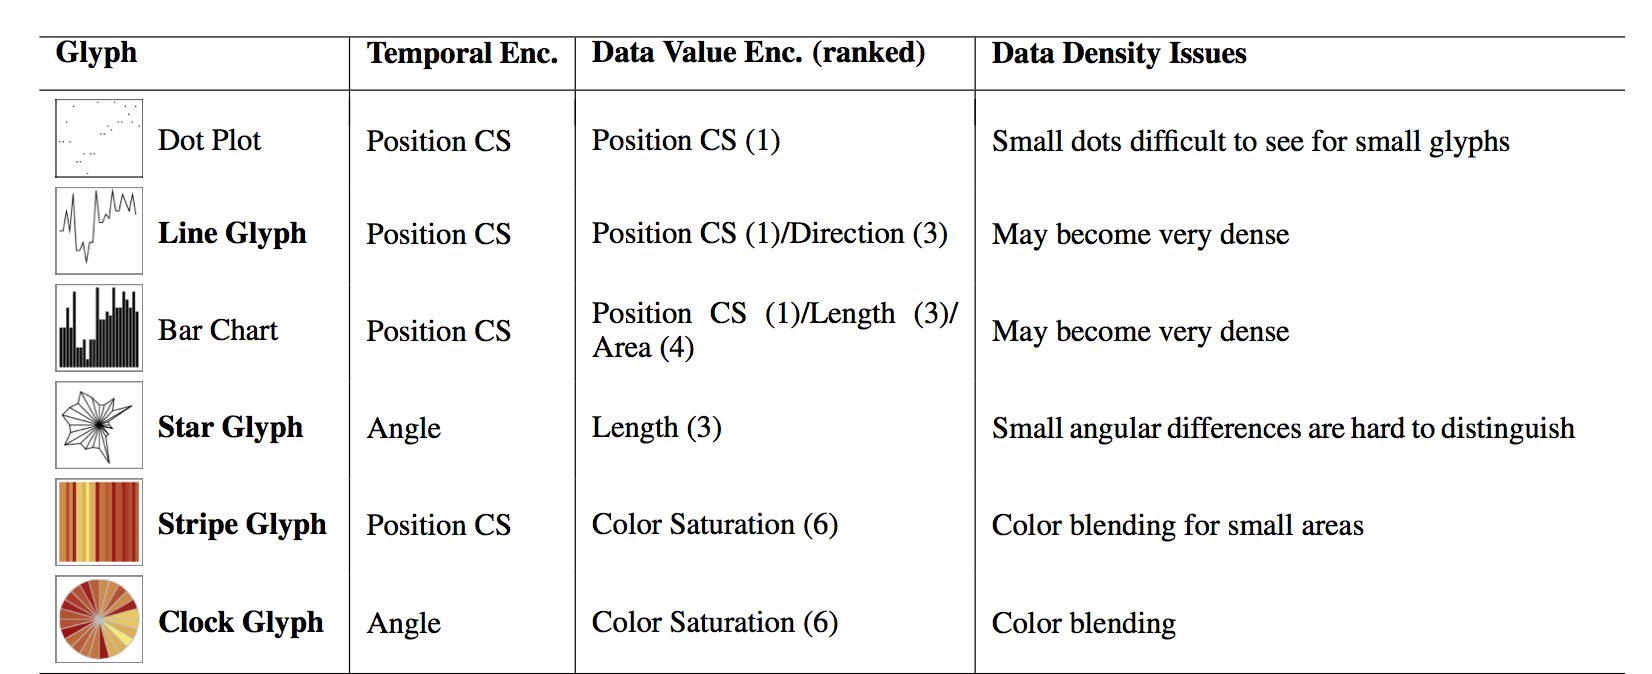
\includegraphics[scale=0.27]{figures/glyph_table.png}
    \caption{Common glyph types and their description.}
    \label{fig:glyphs}
  \end{centering}
\end{figure}

As can be seen in Figure \ref{fig:glyphs}, each common glyph type has their relative strengths and weaknesses.
The important considerations when bringing these visualizations into the Relay Interface is to carefully evaluate the data being presented, and to maximize the saliency of said data, while minimizing issues that may arise with the visualization at at size or density.

Upon making such decisions for the visualization of data, careful planning must be done to place data in locations on the screen and within the application such that the user need not search extensively to find it.
Certain data given by the requirements will be best served on the map, where the context of location and spatial relativity is important.
Other data may be better suited for presentation off of the map, perhaps in a dashboard or modular window setting.
Situations where the context of a single location is important, or in a list-based visualization environment may be areas where data is better suited to be shown away from the map.
These considerations, and more, and discussed further in the following Design Process section.

\subsection{Design Process}
With sufficient Design Research conducted, and functional requirements compiled, the front-end application design moved into an iterative process of defining the user interface (UI), interactions, and visual design of the app through various levels of fidelity.
The use of many design tools was employed, as best suited for each given stage of the design process. 
These tools include Adobe Photoshop and Illustrator, HTML/CSS/JavaScript, and sketching using pencil and paper to quickly illustrate low-fidelity ideas.

\subsubsection{Wireframing}
The process began with a wireframing stage, involving the quick iteration of information architecture and UI techniques, to discover optimal implementations for each of the functional requirements.
Global app navigation, page layout, modularity, and fundamental UI elements were initiated at this stage, to begin to define the design language used in the application.
This was accomplished mainly through static paper-based sketches of various screens.
This allowed for rapid generation of concepts, and movement between and through ideas. 

\begin{figure}[htbp!]
  \begin{centering}
    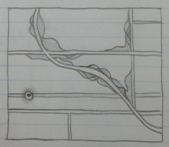
\includegraphics[scale=1]{figures/wire-1.png}
    \caption{Initial wireframe for histogram approach.}
    \label{fig:wire-1}
  \end{centering}
\end{figure}

\begin{figure}[htbp!]
  \begin{centering}
    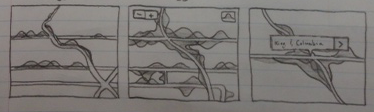
\includegraphics[scale=1]{figures/wire-2.png}
    \caption{Application wireframes showing interaction controls and pop-up menu.}
    \label{fig:wire-2}
  \end{centering}
\end{figure}

As can be seen in Figures \ref{fig:wire-1} - \ref{fig:wire-4}, various overlay techniques using both histograms and circular polygons on a map of a city were explored here in this early stage.
The histogram approach sought to model each vehicle (or small group of vehicles) on the road as a probability density function that could be moved along a road based on knowledge of traffic presence at each intersection, and speed limit data on each road.
More vehicles means more histograms, shown as translucent graphs which when overlaid, become more and more opaque, thus indicating a higher traffic density in that area.

\begin{figure}[htbp!]
  \begin{centering}
    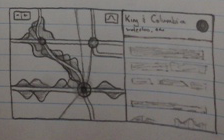
\includegraphics[scale=1]{figures/wire-4.png}
    \caption{Sketch of potential side menu for the Relay Interface application.}
    \label{fig:wire-3}
  \end{centering}
\end{figure}

Response for this concept was generally critical, as probability functions overlaid on a map were found to not be particularly easy to understand, at least not immediately at a glance.
It was evident at this stage that a simpler - more intuitive - visualization was needed for this application to be useful for both consumers and traffic engineers.

\begin{figure}[htbp!]
  \begin{centering}
    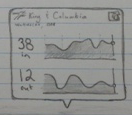
\includegraphics[scale=1]{figures/wire-5.png}
    \caption{Sketch of a detailed pop-up menu showing intersection data.}
    \label{fig:wire-4}
  \end{centering}
\end{figure}

Through exploration of the circular polygon heat-map concept, a more agreeable solution was found.
This concept modelled traffic data on a per intersection basis.
In other words, when an intersection is experiencing a high volume of traffic, a translucent circular polygon is triggered and overlaid onto a map of the city at the longitude and latitude of the intersection.
The size of the circle is positively correlated to the volume of traffic at the intersection.
A second degree of data is then shown through use of colour, to illustrate the performance of the intersection itself.
This gives insight into how well the intersection is moving traffic given it's high-volume state.
It was agreed upon that a well-performing high-volume intersection should receive a colour that is neutral, while a high-volume intersection with poor performance should emit a colour that indicates that something is wrong, such as orange or red.

It can also be seen in the figures that other components of the prototype application were accounted for in the wireframes.
These include interactions such as pop-up dialogues, highlighting routes and communicating intersections, as well as a side-panel for showing detailed metrics on intersection and overall city-wide traffic performance.
From this stage, the prototype moved to a mid-fidelity phase to further build out the concepts and refine the aesthetic of the application.

While not all of these early-stage concepts were used in the final product, the process of generating, critiquing, and refining multiple ideas proved valuable throughout the year.
These initial visualization concepts helped to spawn and guide future implementations, and helped attain a clear understanding of the data being presented.
The next step in the design process moved into a medium-fidelity stage, such that navigation and interaction could be explored at a deeper level.

\subsubsection{Medium-Fidelity Prototyping}
Through the use of prototyping software Balsamiq, a set of interactive mockups were created to both reflect the requirements of the application, as well as ideas and lessons learned from the previous wireframing stage.
In this prototype, the main tenets for the final version of the application were created in an illustrative form, to identify key architectural components and the user's interaction within.
By doing this in a medium that does not put too much focus on the specifics of visual design, it was easier to concentrate on the core features of the application, and how they satisfy (or dissatisfy) the original requirements. 

At this stage, the concept of data layers was explored.
Given that there are many varying metrics identified as important to target users (Traffic Engineers), and that these metrics all have a spatial or location-based relevance, the idea of turning on and off layers of data visualization overlaid on a map was critical in effectively demonstrating traffic data.
Metrics such as intersection Status, and Flow through an intersection were conceptualized at this stage, with some preliminary UI put together for interacting with these layers.
A screenshot of the mockup showing a Status visualization in the Relay app is presented in Figure \ref{fig:bals-1}. \\

\begin{figure}[htbp!]
  \begin{centering}
    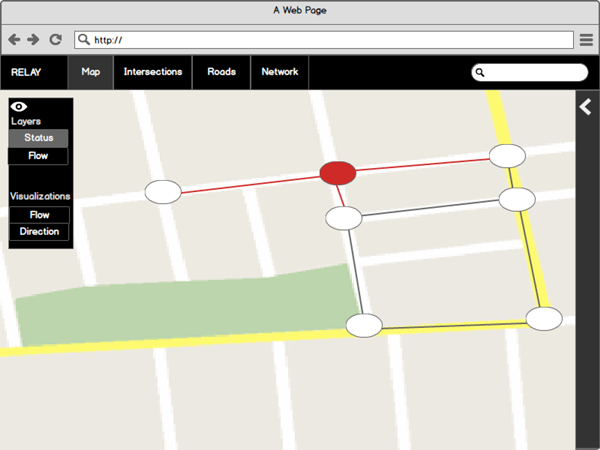
\includegraphics[scale=0.65]{figures/bals-1.png}
    \caption{Balsamiq mockup of a data layer in the Relay app.}
    \label{fig:bals-1}
  \end{centering}
\end{figure}

Additionally, as can be seen at the top of Figure \ref{fig:bals-1} the foundations for global app navigation were built out, in the form of a fixed header bar at the top of the screen.
This header serves many purposes, including branding for the app, search functionality, as well as tabbed buttons to move between contextually grouped pages.
Figure \ref{fig:bals-1} shows the active state of the Map button, while the main area of the screen contains a map with relevant data.

Further interaction design was carried out at this stage, in the form of a modular popup window, referred to as the Relay info box.
This info box was designed to present deeper metrics for an intersection, and appears when an intersection on the map is clicked.
This allows users to quickly inspect any intersection of interest and monitor time-series data in the context of a specific location.
Data provided at this stage includes a graph of the flow of traffic through the intersection in each of the cardinal directions, as well as a matching chart that provides predictive data into the near future, based on stochastic methods from the controller.
The status of the lights is shown, in addition to numerical car counts and the name of the intersection that has been clicked.
A Balsamiq mockup of the info box is presented in Figure \ref{fig:bals-2}. \\

\begin{figure}[htbp!]
  \begin{centering}
    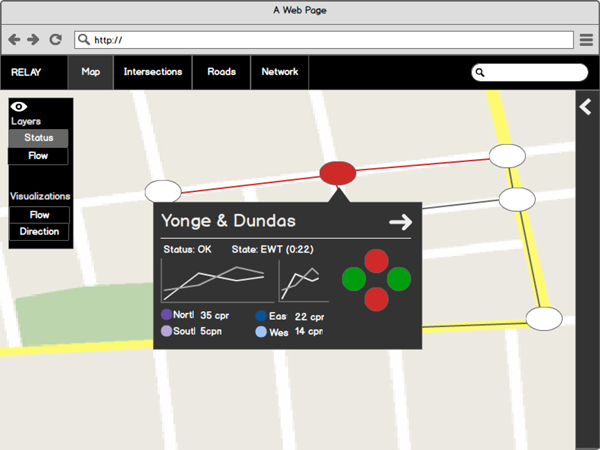
\includegraphics[scale=0.6]{figures/bals-2.png}
    \caption{Balsamiq mockup of the Relay info box.}
    \label{fig:bals-2}
  \end{centering}
\end{figure}

\begin{figure}[htbp!]
  \begin{centering}
    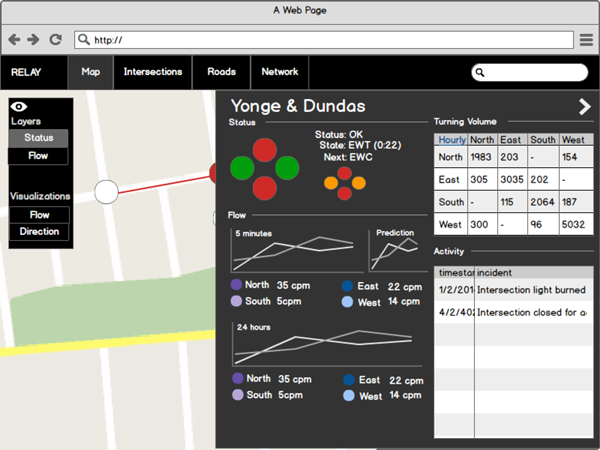
\includegraphics[scale=0.6]{figures/bals-3.png}
    \caption{Balsamiq mockup of the Relay dashboard.}
    \label{fig:bals-3}
  \end{centering}
\end{figure}

While the info box fulfills the need to browse intersections and provide quick snapshots of relevant intersection data, it was important for more advanced users to get an in depth look at this data, such that meaningful trends can be detected and acted upon.
It was necessary for these users - Traffic Engineers - to view metrics on intersection Location, Name, Type, State, In Flow, Out Flow, Predictions, and more.
To accommodate this large quantity of data, a dashboard was prototyped at this stage, setting a preliminary layout for each of the required metrics.
This dashboard slides across the screen from the right by pressing the arrow in the info box, and can then be toggled back and forth with the controls in the upper right corner of the screen.
A Balsamiq mockup of the dashboard can be found above in Figure \ref{fig:bals-3}.
As various intersections are selected on the map, the dashboard updates it's information to reflect that of the intended location.
Time-series graphs update in real-time as data feeds through the system, and an activity log hosts the history of noteworthy incidents at the selected intersection.

With these views on the Map screen prototyped in medium-fidelity, the design progressed into other areas of the application.
Moving through the global navigation buttons along the header, an Intersections page was mocked up.
The goal of this page is to give Traffic Engineers a holistic view on their network, as well as the ability to filter/search and target individual intersections.
This text-based search also allows for insight into any particular intersection by name, as well as the ability to find important groups of intersections or main arteries with many cross streets.
This is important because it allows users to locate intersections in two ways: spatially on the map, and now textually in the intersections table.
A mockup of the Intersections page is shown in Figure \ref{fig:bals-4}, with placeholder data in the intersections table. \\

\begin{figure}[htbp!]
  \begin{centering}
    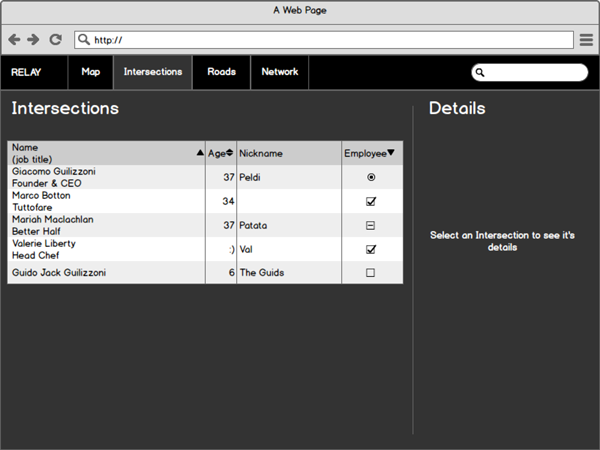
\includegraphics[scale=0.65]{figures/bals-4.png}
    \caption{Balsamiq mockup of the Intersections page.}
    \label{fig:bals-4}
  \end{centering}
\end{figure}

Finally, the medium-fidelity prototyping stage moved on to build out a layout and basic information for a Network page.
The intention of this page is to provide details similar to what would be shown in the info box or dashboard of an intersection, but for the entire network as a whole.
This allows Traffic Engineers to view, understand, diagnose, and make decisions for the network on a macro level, in addition to the finer look provided on a per intersection basis.
A mockup of the Network page is shown in Figure \ref{fig:bals-5}. \\

\begin{figure}[htbp!]
  \begin{centering}
    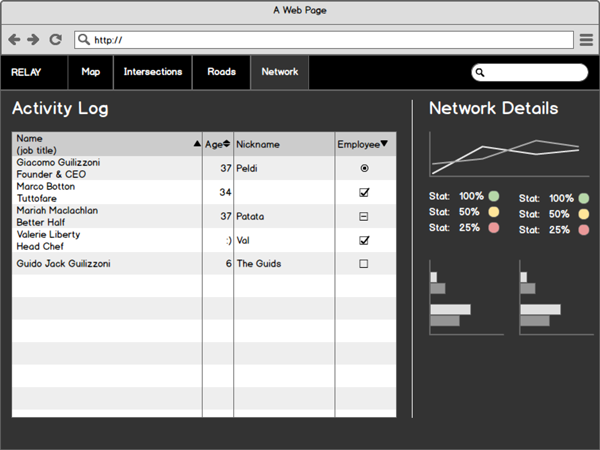
\includegraphics[scale=0.6]{figures/bals-5.png}
    \caption{Balsamiq mockup of the Network page.}
    \label{fig:bals-5}
  \end{centering}
\end{figure}

As can be seen in Figure \ref{fig:bals-5}, a large activity table is provided on the Network page, to highlight issues that occur at all intersections in the network.
These issues include accidents, power outages, abnormal volumes, and more.
Additional detail can be seen on the right hand side of the screen, with quantitative network data placed in charts and numerical tables, and colour-coding of network statuses explored at this stage.

Overall, the medium-fidelity prototyping stage was essential in moving the design of the Relay application forward towards its final state.
With functional requirements set in place, and now a strong roadmap of UI elements, navigation, page layout, and interactions to fulfill the requirements, the application was ready to be built in a high-fidelity form, as described in the following section.

\subsubsection{High-Fidelity Prototyping}
In preparation for the development of the Relay application, the design of the environment moved into a final high-fidelity prototyping phase.
This stage involved a major visual overhaul of the application, focusing on the definition of a unique design language to bring Relay together as a cohesive product.
Considerations at this stage include the creation of a custom grid structure, typography, colour, branding, the development of data visualization layers, and repurposing the search functionality in the app.
The high-fidelity design was done in Adobe Photoshop, Illustrator, and in the browser using HTML/CSS and JavaScript.
These tools allowed for highly accurate creation of assets, development of colour scheme, precise layout of visual elements, and more.

The branding for Relay was created in two main components: the logo, and the typesetting.
The logo is a custom glyph used in the application to denote the state of the signal at an intersection.
It contains four dots in a diamond pattern, with two fully-coloured dots positioned vertically, and two empty dots with a medium-weight stroke positioned horizontally.
In the application, this glyph would represent the flow of traffic in an East-West manner, while North-South traffic is halted at a red light.
This was selected to represent Relay as it both subtly represents what the application does, and provides important information to users in a modern and clean way.
The final Relay branding is shown in Figure \ref{fig:relay-logo}. \\ \\

\begin{figure}[htbp!]
  \begin{centering}
    
\includegraphics[scale=0.7]{figures/relay-logo.png}
    \caption{High-fidelity rendering of the Relay branding.}
    \label{fig:relay-logo}
  \end{centering}
\end{figure}

The typesetting was done to represent Relay in a way that would be clear, trustworthy, confident, readable, and modern.
The use of custom letter positioning through tracking and kerning methods aided this, while promoting clarity and confidence with the capitalization of each letter in the word.
Open Sans, a typeface that is freely available to the public, was utilized for the clean and readable aesthetic it provides.
As a sans-serif font set at a semi-bold weight, each letter is clear from any distance, at many sizes, on both screen and in print.
This also gives the branding a modern feel, as many serifed fonts are often associated with older, more classical and formal scenarios.

The high-fidelity design of the application itself began at a structural level, to set the basis for a consistent, coherent, and unique interface.
A grid structure was optimized for a 1440 x 900 pixel resolution screen - a common resolution on modern screens, and the dimensions of the screens used for the Symposium demo.
The grid was based upon units of 16 pixels, which was decided to be the lowest common denominator for icon and type sizing to ensure usability from many angles and distances.
With a grid structure in place, all following design decisions then had a reference point to follow from.
This aided in the purposeful use of negative spacing, symmetry, and balance of each screen composition.
The grid on a blank canvas is shown in Figure \ref{fig:dot-grid}. \\

\begin{figure}[htbp!]
  \begin{centering}
    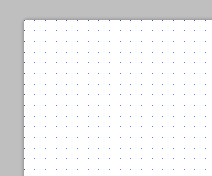
\includegraphics[scale=1]{figures/dot-grid.png}
    \caption{16 pixel grid foundation for the Relay user interface.}
    \label{fig:dot-grid}
  \end{centering}
\end{figure}

The first consideration in developing the design language for the application was the typography.
Just like the branding, the typography was intended to be clear and readable, but also neutral in tone.
Neutrality of the type allows for clear representation of the content itself, which is highly important in such a data-heavy application.
As a critical element of the user interface, particular attention was paid to hierarchy of type sizes and weights, all deriving from a smallest line-height of 16 pixels, used in small data labels and body.
The typeface Helvetica Neue was used, as it is well-known to provide very clear and readable text at many sizes, with a neutral tone.
Additionally, it is a common typeface used in the signage of many major cities around the world.
This gives the application a recognizable and associative feeling, which is especially important for an application that deals with traffic conditions in urban areas.
An example of an intersection name set in 24pt Helvetica Neue Bold is shown in Figure \ref{fig:name}. \\

\begin{figure}[htbp!]
  \begin{centering}
    
\includegraphics[scale=1]{figures/name.png}
    \caption{An intersection name set in 24pt Helvetica Neue Bold.}
    \label{fig:name}
  \end{centering}
\end{figure}

The high-fidelity prototyping process continued with the development of colour-scheme for the application.
Given the importance of visualizing data in the Relay app, it was decided that all non-data elements of the UI - the map, modular overlays, and header, for example - should be subdued and clearly grouped together as functionally similar elements.
To accomplish this, a black and white UI was established for all control elements, providing a clean environment for navigation, while vibrant, highly-saturated colours were used for charts and data layers.
This technique effectively created a high-contrast environment where areas that require visual focus, attention, and thought - i.e. the data - were the most salient elements on the screen, and any layout or navigational components were done in a clear black and white manner, similar to signage found on the streets of many major cities.
Therefore, all contextually similar elements were easily grouped and identifiable through their similarities or differences in colour.
An example of a chart showing the flow of traffic through an intersection over time is illustrated in Figure \ref{fig:chart}.
Notice the vibrancy of the coloured data, and its contrast with the structural page elements surrounding it. \\

\begin{figure}[htbp!]
  \begin{centering}
    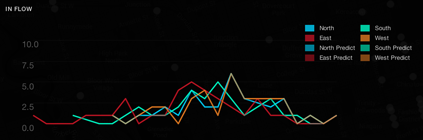
\includegraphics[scale=0.9]{figures/chart.png}
    \caption{A chart showing the flow of traffic through an intersection over time.}
    \label{fig:chart}
  \end{centering}
\end{figure}

The data visualization layers were next to be developed at the high-fidelity stage.
These visualizations took the form of heat maps, as well as quantitative, relative, and boolean glyphs, representing data on the Status, Flow, and Queue Length at a given intersection.
The first visualization layer, showing the Status of intersections, used small dot glyphs of different colour to display the boolean status of a light.
By overlaying a dot at each intersection, with a corresponding white or red colour to denote proper working condition vs. an error, such as a power outage, an easily digestible visualization was created.
This empowers Traffic Engineers to easily monitor their network, and to detect any anomalies that may have occurred.
A screenshot of the Status layer is shown in Figure \ref{fig:status}. \\

\begin{figure}[htbp!]
  \begin{centering}
    
\includegraphics[scale=0.9]{figures/status.png}
    \caption{A screenshot of the intersection Status data layer.}
    \label{fig:status}
  \end{centering}
\end{figure}

The second data layer to be designed was a heat map representing the flow of traffic through intersections.
This was accomplished on a per-intersection basis, and was intended to provide a macro view of the relative traffic density across areas of the city.
This view is most useful for those looking for an overview of general traffic conditions, such as a browsing Traffic Engineer, or a consumer looking to plan a route through the city.
A screenshot of the first Flow visualization layer is shown in Figure \ref{fig:flow-1}.

\begin{figure}[htbp!]
  \begin{centering}
    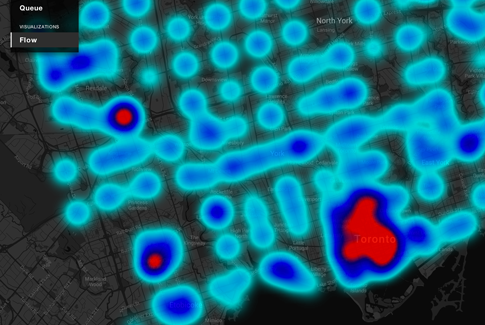
\includegraphics[scale=0.9]{figures/flow-1.png}
    \caption{A screenshot of the flow per-intersection heat map.}
    \label{fig:flow-1}
  \end{centering}
\end{figure}

Following this Flow visualization, a second implementation of traffic flow was developed, this time looking at flow between intersections, rather than at or through any particular intersection.
This was accomplished by taking predictive data from the controller, and approximating the position of cars along roadways given the knowledge of their entry and exit directions from each intersection.
Each car is plotted as a low-opacity glyph of concentric circles, with a bright green core, a lighter green exterior, and a soft blue outline, denoting the estimated nature of the position of any given car.
Given the large number of vehicles to be accounted for, a low opacity was selected for each individual glyph, so that as they overlap with one another, the intensity of the colour increases so as to illustrate the increasing density of traffic in an area.
A screenshot of the Flow between intersections data layer is shown in Figure \ref{fig:flow-2}.

\begin{figure}[htbp!]
  \begin{centering}
    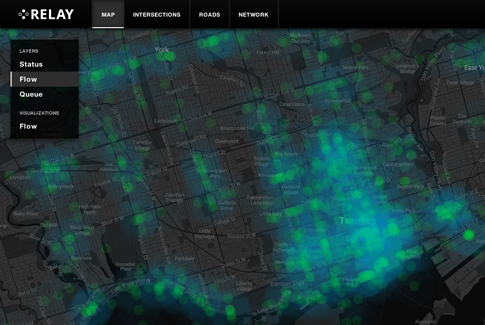
\includegraphics[scale=0.9]{figures/flow-2.png}
    \caption{A screenshot of the flow between intersections heat map.}
    \label{fig:flow-2}
  \end{centering}
\end{figure}

As can be seen in Figure \ref{fig:flow-2}, the natural visualization of major roadways and arteries through the cities is evident, which is an important result of this visualization.
A wide range of traffic patterns can be derived from this, thanks to the high-resolution of data points that give a continuous feel to the data, as opposed to the limited two-stage discrete options currently available through applications such as Google and Apple Maps.

Finally, the final visualization layer looked to showcase the data representing Queue Length or average wait time at an intersection.
The goal of this visualization was to produce glyphs that could show both quantitative measures, as well as give a sense of relative weighting between intersections.
A four-pronged glyph was developed, with three short prongs extending in the East, South, and West directions, while a variably sized prong extends to the North.
The length of the North prong corresponds to the average wait time at a given intersection, while the three shorter prongs are of equal length and serve as a stand for the quantitative North measure.
This creates a pseudo 3-dimensional effect, and gives the user a unique look at the changing landscape of queue lengths in the city - similar to how a city skyline may look with many tall buildings.
A screenshot of the Queue Length visualization layer is shown in Figure \ref{fig:queue}.

\begin{figure}[htbp!]
  \begin{centering}
    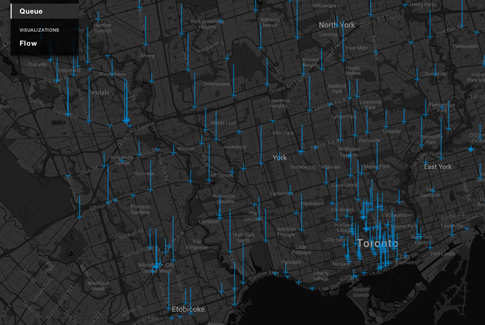
\includegraphics[scale=0.9]{figures/queue.png}
    \caption{A screenshot of the average queue length at each intersection.}
    \label{fig:queue}
  \end{centering}
\end{figure}

Following the design of the data visualization layers, the high-fidelity stage looked at the search functionality of the application, and focused attention on repurposing its form to better reflect its function.
Previous prototypes held the search bar in the header across all pages of the application.
This proved to be troublesome, as some pages did not require any search functionality, while the ones that did actually served as text-based filters within the context of the current page.
The high-fidelity design saw the removal of the search bar from the global navigation header, and into the upper section of the Intersections and Network pages.
This way, the text-based tables found on these pages could be easily searched/filtered, without the confusion of entering text into the global header, where a new page would be the expected result.

An additional feature that made its way through the high-fidelity phase is the Connection Status window.
This window is activated through the gear icon in the top right corner of the screen, and is useful for monitoring the status of the connection between the front-end and back-end of the application.
This window is positioned in the top-right of the screen so as to avoid covering any important visual elements, and is padded in from the top and right sides of the screen to maintain access to the dashboard toggle button.
The connection status window identifies where the data is coming from: either through a Web Socket or through the application's REST API.
It also identifies time since the last data update, both locally on a selected intersection, and globally over the entire network.
A screenshot of the Connection Status window is shown in Figure \ref{fig:connection}.

\begin{figure}[htbp!]
  \begin{centering}
    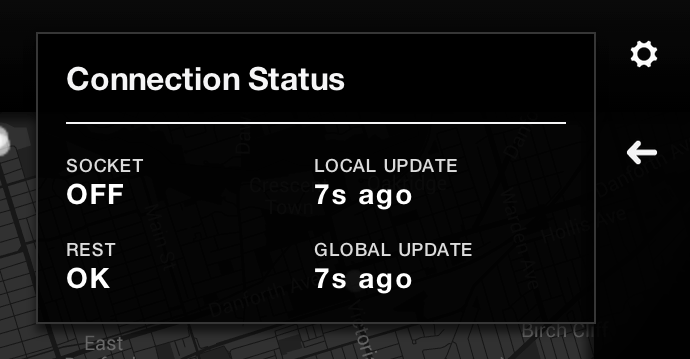
\includegraphics[scale=0.6]{figures/connection.png}
    \caption{A screenshot of the connection status window.}
    \label{fig:connection}
  \end{centering}
\end{figure}

Lastly, the intersection dashboard was refined at a high-fidelity stage.
The specific metrics contained in the dashboard were iterated on and refined from the medium-fidelity stage to accurately reflect the data coming from the back-end controller.
This involved splitting the Flow metric into In-Flow and Out-Flow at an intersection, showing the current and next intended State of the traffic lights, and providing a new Turn Predictions matrix, which gives the predicted quantity of cars moving through each permutation of turns based on stochastic data from the back-end.
In-line with the medium-fidelity prototype, the Activity Log is provided giving consideration to readability and interaction, with subtle hover states on individual table rows to improve salience of desired fields.
Additional information includes the Intersection ID and the Intersection Type, two identifiers that are often important to Traffic Engineers.
A screenshot of the high-fidelity dashboard is shown in Figure \ref{fig:dashboardt}. \\

\begin{figure}[htbp!]
  \begin{centering}
    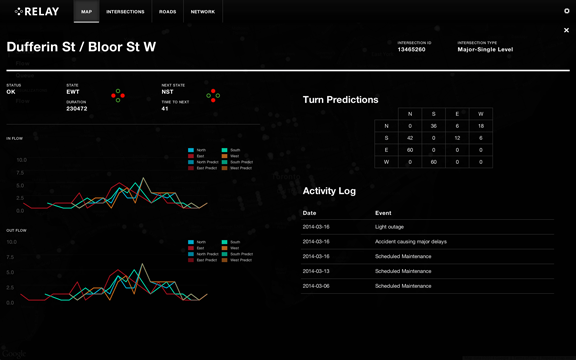
\includegraphics[scale=0.73]{figures/dashboard.png}
    \caption{A screenshot of the Relay intersection dashboard.}
    \label{fig:dashboardt}
  \end{centering}
\end{figure}

With these elements in place, the final developmental/functional touches to the Relay application were ready to be built for the demo, as showcased on Symposium day.
As a unit, the application is held together using the modular design elements described above, which makes the application easily scalable and modifiable for individual implementations or changing metrics and requirements.
With a unique and well-defined design language established, further extrapolations of this implementation have a library of best practices and UI elements that can be carried forward into new scenarios.

\subsection{Application Design}

Application interfaces for critical infrastructure such as a traffic control network must be highly robust and reliable. Furthermore, it is important the the systems are able to scale in order to accommodate the inevitable growth of the system. These main ideas drove the design of the Front End (web application) application architecture. 

Design research and prototpying highlighted the need for various technologies to be used in the development of the Front End. For example, the presence of a map-based interface meant that a mapping library was required. Given the functional and technical requirements of the project, it was important to select solutions which met the project's needs. Given the breadth of choices in software technology, it was necessary to use a quantifiable selection process for determining the appropriate solutions from a group of candidates. The three main areas of the front-end application which required such a process are the Framework, Mapping Library, and Visualization Library. The selection process for these is discussed in the following sections.

\subsubsection{Framework Selection}

Software frameworks are code libraries which provide functionality that enables developers to more easily implement a specific software pattern. One of the most common software patterns is the Model-View-Controller (MVC) pattern, which is commonly used in complex and large software applications to ensure the application is reliable, structured, and can scale effectively. Similarly, front-end software frameworks allow for the development of structured and scalable applications by providing software pattern utilities. Given the critical nature of our application, it was determined that the use of a framework would be appropriate for ensuring the scalability and reliability of the application.

Four JavaScript frameworks were selected for comparison. Javascript MVC is a mature, well-known front-end MVC implementation which is built off of jQuery, a JavaScript Utility Library, which offers a well-rounded feature base. DOJO is another mature and well-known framework which does not offer an MVC-style framework, yet is class-oriented. Backbone.JS is a relatively new Model-View (MV) framework built off of the Underscore.js utility library. Finally, Angular.js is a new and highly functional front-end framework which loosely follows an MVC pattern.

The frameworks are scored across five weighted features. The scores are justified and a winning framework is selected.

\begin{enumerate}

\item \textbf{Size} - The use of large JavaScript libraries can cause performance issues within the application. The selected library should be as small as possible. Candidate frameworks will be assessed based on the size of their encompassing code files. This feature has been given a weight of 0.5.

\item \textbf{Independence} - The selected framework should be self-contained and not require many prerequisite JavaScript Libraries in order to function. The presence of many prerequisite libraries increases the size of the application and will slow down performance. Candidate frameworks are assessed based on the number of prerequisite frameworks and plug-ins required for the framework's implementation within the proposed solution. This feature has been given a weight of 0.5.

\item \textbf{Functionality} - The selected JavaScript framework should provide a rich set functionality which is not available within the native JavaScript language. Important functionality includes utility functions, templating, Document Object Model (DOM) binding, client-server communication methods, and data structure classes. Candidate frameworks are assessed based on the both the quantity and quality of the functionality provided, in the context of the proposed solution. This feature has been given a weight of 0.8, as it is important that the framework provides sufficient functionality to implement the solution.

\item \textbf{Modularity} - It is important that the selected JavaScvript framework supports the creation of modular code, given the complexity of the proposed solution. The selected MVC framework should encourage an established code pattern, such as and MV- or MVC-style structure. Candidate frameworks are assessed based on their similarity to known software architecture patterns, such as MV or MVC. Due to the importance of scalability and modularity in the proposed solution, this feature has been given a weighting of 0.8.

\item \textbf{Implementation Overhead} - The selected JavaScript framework should not require excessive amounts of overhead code in order to successfully suit the needs of the proposed solution. The selected framework should have as little overhead as possible. Candidate frameworks are assessed by examining tutorial code implementations for each framework, to determine the proportion of development required as overhead compared to application-specific code. This feature has been given a weight of 0.5.

\end{enumerate}

The frameworks are presented in a weighted decision matrix below. Each attribute is weighted out of 5 points for each of the candidate frameworks. Weightings for each attribute are on a scale from 0 to 1.

\begin{table}
\centering
    \begin{tabular}{l|llll}
    ~                             & Angular.js & \textbf{Backbone.js} & DOJO    & JavaScript MVC \\ \hline
    Size (0.5)                    & 5 (2.5)    & \textbf{3 (1.5)}     & 2 (1)   & 2 (1)        \\
    Independence (0.5)            & 5 (2.5)    & \textbf{4 (2)}       & 3 (1.5)   & 4 (2)          \\
    Functionality (0.8)           & 3 (2.4)    & \textbf{5 (4)}       & 4 (3.6)   & 4 (3.6)          \\
    Modularity (0.8)              & 2 (1.6)    & \textbf{4 (3.6)}     & 4 (3.6) & 4 (3.6)        \\
    Implementation Overhead (0.7) & 4 (2.8)    & \textbf{4 (2.8)}     & 3 (2.1) & 4 (2.8)        \\ \hline
    Totals                        & 11.8       & \textbf{13.9}        & 11.8    & 13.0           \\
    \end{tabular}
\caption{Weighted Decision Matrix for JavaScript Framework Selection}
\label{table:framework-matrix}
\end{table}

Angular.js is the smallest candidate framework at 36kb. Angular.js also has no prerequisite JavaScript libraries, and is thus completely independent. Although Angular.js offers rich DOM and interaction functionality, it provides few utility features for data structures and architectures. Angular.js does not follow a rigid MVC or MV structure, which was a major downfall for the framework. Anjular.js does not require much overhead code to implement, primarily because it does not follow a rigid software architecture, and thus is more functionally-oriented.

The Backbone JavaScript framework is 64kb in size. Backbone.js relies on Underscore.js and jQuery.js two relatively large JavaScript utility libraries. However, both of these libraries will be used in the application regardless of the choice of framework, thus are not a direct detriment of this candidate. Backbone.js follows a MV framework style, where both controller and view functionality are both kept in the view. This pattern is a good compromise between no framework and an extremely heavy MVC structure. Backbone.js's two utility libraries provide rich functionality for working with the DOM model and structured objects. Furthermore, Backbone.js provides a native and collection-oriented pattern developed specifically for handling large numbers of similar objects, which fits well with the application's need to support many intersection and road models. Finally, Backbone.js has minimal development overhead considering it's MV structure, as Backbone.js provides a range of default functionality for its classes.

The DOJO JavaScript framework is 155kb in size, making it the largest of the candidate frameworks. DOJO requires no prerequisite JavaScript Libraries, yet many of DOJO's features are in add-on libraries. This reduces the effectiveness of DOJO's core code, yet means a wider range of features are available as the feature set distributed and open. However, DOJO's functionality is not aimed specifically at dealing with large collections of data, and does not offer strong support for client-server synchronicity. In terms of modularity, the DOJO framework supports the creation of class objects yet does not explicitly support an MV- or MVC-style framework. DOJO requires a significant amount of implementation overhead, which makes it suitable for extremely large and diverse applications. However, this level of overhead is less suited to the complex yet relatively consistent nature of our application with respect to object and data needs.

JavaScript MVC is 105kb in size. JavaScrvipt MVC relies on the jQuery.js JavaScript library, however this library is already a requirement for the proposed solution. JavaScript MVC is composed of four sub-frameworks, each of which specializes in a different set of features, and together provide sufficient functionality for the proposed solution. However, like DOJO, JavaScript MVC lacks the specific functionality for dealing with large amounts of similar objects. As suggested by the name, JavaScript MVC follows a strong MVC model in it's implementation.

As seen in table \ref{table:framework-matrix}, Backbone.js is the winning candidate. Backbone.js is not the smallest candidate, yet it's feature set and MV framework fit well with the needs of the proposed solution. Specifically, Backbone's use of already-implemented JavaScript utility libraries to provide enhanced data structure tools and algorithms, as well as it's specialized collection template for dealing with large amounts of data objects. Furthermore, Backbone.js provides functionality for client-server communication for said collection structures. Finally, the overhead associated with Backbone.js is acceptable given the strong fit of the functionality with that of the proposed solution.

\subsubsection{Mapping Library Selection}

Next, a JavaScript mapping library needed to be selected. The proposed solution required that information be viewed in a geographic context. Thus, it was necessary to select a client-side library which would support these needs. Generally, it was important the the library be highly-customizable, as the data presentation layers would be completely customized. Furthermore, the library had to be high-performance in order to support the needs of our application. Finally, it was necessary to find a tile hosting service which could support the library, as setting up a hosting service was not in the scope of this solution.

\begin{enumerate}

\item \textbf{Style Customizability} - The selected mapping candidate should be highly customizable. Colour and styling for map features such as roads, buildings, water, and land must be allowed. This feature has been given a weight of 0.5 as it is not crucial, yet still important to the aesthetic value of the interface.

\item \textbf{Feature Customizability} - The selected mapping candidate must allow for the customization of built-in features, such as markers and info boxes. Markers should be completely customizable, through the use of either a scalable vector graphic (SVG) or HTML and CSS. Info boxes should be customizable using HTML, CSS, and JavaScript. This feature has been given a weight of 0.7 for it's importance in defining the customizability of crucial interface features.

\item \textbf{Layer Customizability} - The selected mapping candidate must allow for the customization of map data layers. The candidate must support multiple simultaneous layers of data. It should also support the display of both point-based and vector-based data. This feature has been given a weight of 0.9, as the value of the application is directly related to the presentation of the various data layers.

\item \textbf{Tile Hosting Support} - The selected mapping candidate must either support tile hosting as part of its service, or be compatible with an existing tile hosting service. Ideally, the selected candidate offers both tile hosting and serving in the same package for convenience. This feature has been given a weight of 0.6, as it is not a crucial feature yet saves significant effort if present.

\item \textbf{Price} - The selected mapping candidate must be cost effective. The service should be free, or minimize the cost of tile serving and hosting. This feature has been given a weight of 1 due to the highly restrictive budget for the proposed solution.

\end{enumerate}

Three Mapping Libraries were considered as potential candidates: Google Maps API, Leaflet.js with CoudMade for tile serving, and Mapbox with TileMill.

The Google Maps API is the industry standard of mapping libraries. It is the same framework which runs Google Maps, and thus it is well-supported and reliable. The Google Maps API allows for styling customizations on-the-go through it's JavaScript API. Unfortunately, not all aspects of the map are stylable. The API provides functionality for both markers and info boxes. The Google Maps API allows for custom CSV marker icons, however the info box is not easily customizable. However, Google Maps does offer a plug-in info box, which is fully customizable. Tiles are hosted directly through Google Maps, requiring no extra work for tile hosting support. Finally, the Google Maps API is a free service with very high courtesy limits.

Leaftlet.js is a map-oriented JavaScript library which provides a variety of map-related features on top of a tile service. Leaflet.js does not host map tiles, and thus it must be used in conjunction with a tile hosting service such as CloudMade. As such, styling the map must be done through a CloudMade's third party service, which is restrictive in styling. Leatlet.js offers rich map functionality, including markers and info boxes. Furthermore, Leaflet.js' map features are highly-customizable, as it is an open-source project. However, Leaflet.js is not geared towards handling data layers. Leaflet.js is a free library.

Mapbox is a new JavaScript mapping library which works in conjunction with TileMill, a tile styling styling service. TileMill is designed specifically for creating highly-customized map styles, and thus offers very rich styling capability. Due to Mapbox's immaturity as a platform, it's feature set is limited and not very customizable. The MapBbox JavaScript library is not structured towards handling data layers, rather individual data points. Furthermore, TileMill tiles must be hosted using a third-party platform, or through MapBox directly, which required a paid membership for the service.

\begin{table}
\centering
    \begin{tabular}{l |r r r l}
    ~                             & \textbf{Google Maps API} & Leaflet.js \& CloudMade & Mapbox \& TileMill \\ \hline
    Style Customizability  (0.5)  & \textbf{3 (1.5)}         & 3 (1.5)                 & 5 (2.5)            \\
    Feature Customizability (0.7) & \textbf{4 (2.8)}         & 5 (3.5)                 & 3 (2.1)            \\
    Layer Customizability (0.9)   & \textbf{5 (4.5)}         & 4 (3.6)                 & 3 (2.7)            \\
    Tile Hosting Support (0.6)    & \textbf{5 (3.0)}           & 3 (1.8)                 & 3 (1.8)            \\
    Price (1)                     & \textbf{5 (5.0)}           & 4 (4.0)                   & 3 (3.0)              \\ \hline
    Total                         & \textbf{16.8}            & 14.4                    & 12.1               \\
    \end{tabular}
\caption{Weighted Decision Matrix for Mapping Library Selection}
\label{table:mapping-matrix}
\end{table}

The candidate mapping libraries are compared in Table \ref{table:mapping-matrix}. The Google Maps API is the winning mapping library. Although the Google Maps Llibrary lacks full native customizability for both it's map styling and map features, sufficient customizability is found within the native functionality and through the use of add-on libraries. The Google Maps API provides excellent data layer functionality, which is unparalleled in feature breadth and support. Finally, the Google Maps combined tile hosting and JavaScript functionality provided within a free service make it the clear choice.

\subsubsection{Visualization Library Selection}

Given the proposed solution's heavy focus on data presentation and visualization, it was important to select a visualization library which supported a wide range of data visualization formats. It was necessary to select a library which allowed for heavy style customization, including line format, colours, grid styles, and legend displays. Considering that traffic information exists in the temporal space, it was important that the library handle time series data well. Specifically, functionality for handling timestamp formatting and real-time or high-frequency updating.

The candidate visualization libraries are assessed across 5 feature categories.

\begin{enumerate}

\item \textbf{Prerequisites and Add-Ons} - The selected visualization library should require minimal additional plug-ins or libraries to run. All of the necessary functionality should be available within the core library files. Candidate libraries will be assessed based on the number of additional files or libraries required to perform. This feature has been given a weight of 0.5, as the functionality of the library is relatively more important than the quantity and size of the library's dependencies.

\item \textbf{Implementation Complexity} - The selected visualization should minimize the amount of code required to produce the necessary visualization. Unnecessarily long setup scripts may cause performance issues in the application. Candidate mapping libraries will be assessed by examining example code and tutorials in order to understand the complexity of visualization implementation.This feature has been given a weight of 0.8, due to the frequency and extent of visualization use within the proposed solution.

\item \textbf{Time-Series Support} - The selected visualization library should have rich time-series support. The library should support timestamps in various data formats and allow for the display of time values in a variety of formats. Candidate mapping libraries will be assessed based on the extent of the documented time-series formatting functionality available for the library. This feature has been given a weight of 0.9, as time-series support is crucial for the proper display of information within the proposed solution.

\item \textbf{Style Customizability} - The selected visualization library must allow for highly customized visualizations. The library should allow for the customization of visualization style, line style, legend style and placement, grid style and placement, and axis style and placement. Candidate mapping libraries will be assessed based on the extent of documented customizable features available for the library. This feature has been given a weight of 0.8, due to the importance of data presentation style in the success of the proposed solution.

\item \textbf{Ease of Updating} - The selected visualization library must support real-time updating of the data within the visualization. The library should either explicitly support data updating through JavaScript methods, or allow for the replacement of the data object and the redrawing of the visualization. Candidate libraries will be assessed based on the perceived presence of such functionality within the library documentation. This feature has been given a weight of 0.9, as the proposed solution relies on the real-time display of information.

\end{enumerate}

Four JavaScript-based visualization libraries were assessed as candidates.

Chart.js is an HTML5-based visualization library, focused on delivering implementations of several core data presentation formats, e.g. bar charts and line charts. Chart.js is a stand-alone library, requiring no outside code. The implementation of visualizations in Chart.js is easy and requires minimal amounts of code. Chart.js does not support any formatting for axis labels, including support for date formatting and time-series support. Chart.js provides an intermediate amount of formatting options for visualizations, however the restriction of the library to 6 main visualization formats limits the presentations options while using this library. Furthermore, Chart.js does not support the updating of chart data in any way, and would require the chart to be recreated in order to display new data.

D3, or Data-Driven Documents, is the most well-known and feature-rich HTML visualization library today. D3 provides an extremely wide range of visualization formats which are completely customizable. D3 has no pre-requisite libraries, and is a stand-alone library. D3's main downfall is the complexity of implementation, as basic data presentations can require up to 300 lines of code. As an extension of D3's extreme customizability, it is possible to use time-series data, however the library provides little native formatting support. D3 provides the widest range of visualization options by far. Finally, D3's support of data updating depends on the visualization method used, however it is generally poor due to the static nature of the library.

Flot is a JavaScipt-based visualization library built on top of the jQuery utility library. Flot is a medium-complexity visualization library which emphasizes informative and real-time visualizations. As mentioned, the Flot library requires jQuery to run, however jQuery is already a prerequisite for multiple other libraries and feature in the proposed solution. Flot charts are not designed to be extremely easy to implement; their implementation complexity is significant, yet more efficient than other candidates and understandable given the functionality available. Flot natively offers moderate time-series formatting support: Flot accepts JavaScript timestamps as time-series data, and is able to format said data in a variety of styles. With the addition of a jQuery plugin, the range of styles is greatly increased. Flot provides a moderate amount of customizability for their data presentations. However, due to the open-source nature of Flot, the inner styling variables are publicly known, which allows them to be customized far beyond what is supported through public JavaScript methods. Finally, Flot handles data updating very well, with explicit JavaScript functions for updating data objects and re-rendering visualizations.

Rickshaw is a new, static, visualization library build using D3 functionality. It aims to offer less complex implementations of basic data visualizations using the D3 framework. Obviously, D3 must be loaded in order for Rickshaw to run, which brings the negative performance implications of loading such a large library as D3. Rickshaw data presentations are exceptionally easy to define and require minimal code. However, the immaturity of the library means that only a few plotting styles are supported, greatly limiting the library's capability. Furthermore, Rickshaw is a private library and is thus less accessible to customizing beyond the limited exposed styling options. Rickshaw does provide time-series formatting support, however it is limited in scope and buggy as the library is not yet a mature project. Finally, due to the static nature of the underlying D3 platform, the Rickshaw library has no support for updating the data object, and thus would require the recreation of the visualization.

\begin{table}
\centering
    \begin{tabular}{l | r r r r}
    ~                               & Chart.js & D3      & \textbf{Flot}    & Rickshaw \\ \hline
    Prerequisites \& Add-Ons (0.5)  & 5 (2.5)  & 5 (2.5) & \textbf{4 (2.0)} & 4 (2.0)  \\
    Implementation Complexity (0.8) & 4 (3.6)  & 1 (0.8) & \textbf{3 (2.4)} & 5 (4.0)  \\
    Time-Series Support (0.9)       & 1 (0.9)  & 3 (2.7) & \textbf{5 (4.5)} & 3 (2.7)  \\
    Style Customizability (0.8)     & 2 (1.6)  & 5 (4.0) & \textbf{4 (3.6)} & 3 (2.4)  \\
    Ease of Updating (0.9)          & 1 (0.9)  & 2 (1.4) & \textbf{4 (3.6)} & 1 (0.9)  \\ \hline
    Total                           & 9.5      & 11.4    & \textbf{16.1}    & 12.0     \\
    \end{tabular}
\caption{Weighted Decision Matrix for Visualization Library Selection}
\label{table:visualization-matrix}
\end{table}

Assessment of the candidate visualization libraries is done through a Weighted Decision Matrix, as seen in Table \ref{table:visualization-matrix}. As seen in Table \ref{table:visualization-matrix}, Flot is the winning visualization candidate. Flot's exceptional functionality with regards to time-series data and data updating fit well with the needs of the proposed solution. Furthermore, the Flot visualization library provided a suitable balance of complexity and customizability for the proposed solution.

\subsection{Application Development}

The Front End application is composed of two parts: static HTML and CSS, and a JavaScript architecture. The HTML and CSS code's role is for composition and stying of the interface, whereas the JavaScript is responsible for controlling the interface. This pattern is standard for web applications, and thus provides a good reference for the development of Relay's Front End infrastructure.

In the early stages of prototyping the Front End application, the application was composed primarily of HTML and CSS code. This allowed for the creation of a visually-appealing interface which could be assessed as a proof-of-concept demonstration. As the application became more complex, emphasis shifted towards the use of JavaScript for initializing and implementing the interface. The HTML and CSS structure expanded to support the interface as it grew in complexity. The style of the HTML/CSS structure shifted towards template-based widgets, which could be dynamically controlled via JavaScript functionality.

The architecture for the Front End application saw three major iterations. Each phase represents a more complex yet refined application architecture. Tables \ref{fig:iteration1}, \ref{fig:iteration2}, and \ref{fig:iteration3} document the Javascript architecture at each iteration.

Due to the use of Backbone.js as the JavaScript framework, the application follows an MV architecture, where only models and views exists as distinct classes, and controller functionality is included in the view object. Backbone.js includes a specific model pattern called a collection, which is an object responsible for handling multiple models of the same class. The solution leverages the functionality provided by the collection pattern, and they have been appropriately categorized in the architecture diagrams. However, collections are similar to models in the sense that they have no controlling functionality, and thus are treated like models in the sense that each as an accompanying view class to handle it's controlling functionality.

The 'User Entry' mark within the architecture diagrams indicates the entry point to the initialization of the JavaScript code. This is done using a call to the script (iteration 1) or through the initialization of the indicated class object (iterations 2 and 3), which then progressively initializes all other classes within the structure. The arrow direction indicates the direction of ownership within the classes. That is, class A pointing to class B indicates that class A owns one or multiple instances of Class B. At the bottom of each diagram, database connection points are indicated. The presence of a line between a model and a database indicates the ability for the model to query the database. Finally, views which are directly owned by a collection view are stacked. This is to show the collection view's 1-to-n relationship with the view classes in the implementation.

The first major implementation was a proof-of-concept interface developed for the Fall Demonstration and Presentation. The goal was a low-fidelity simulation of the core functionality in the solution. Thus, the code was developed in a less-structured manner so it could be changed quickly as various implementation strategies were tested. As seen in Figure \ref{fig:iteration1}, all functionality was developed in a single, class-less script. No specific class pattern was implemented at this stage.

\begin{figure}[htbp!]
  \begin{centering}
    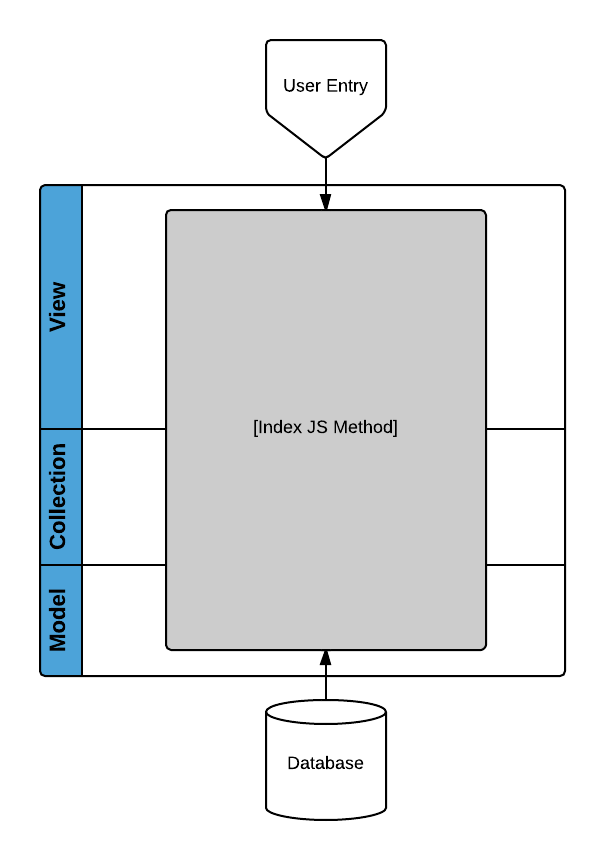
\includegraphics[scale=0.25]{figures/Iteration-1.png}
    \caption{An architectural diagram for Iteration 1.}
    \label{fig:iteration1}
  \end{centering}
\end{figure}

The second major implementation was completed for the Winter Demonstration and Presentation. A more mature class architecture had been developed, seen in Figure \ref{fig:iteration2} as many of the necessary utility libraries had been selected. Furthermore, Backbone.js had been selected as the JavaScript framework of choice, and significant effort had been made into transitioning the original functionality into the Backbone.js pattern.

The App View class is primarily responsible for handling the initialization of the application, and acts as a wrapper for all other functionality. This iteration contained a single screen, and the screen was appropriately given a view class to manage it's interface and interactions with the model. Furthermore, intersections pulled from the database were stored in a collection class, where each intersection was represented with an intersection model. The intersection class created an intersection view for each model, which handled direct interactions from the interface on a specific intersection. 

It is important to note that the model and collection classes are initialized at the app level. This allows for the model objects to be used as singleton instances of the network information, removing the need for redundant data in the interface, as well as reduction in data transfer between the client and server. Furthermore, this strategy improves the robustness of the client application though restricting server communication to a single channel.

\begin{figure}[htbp!]
  \begin{centering}
    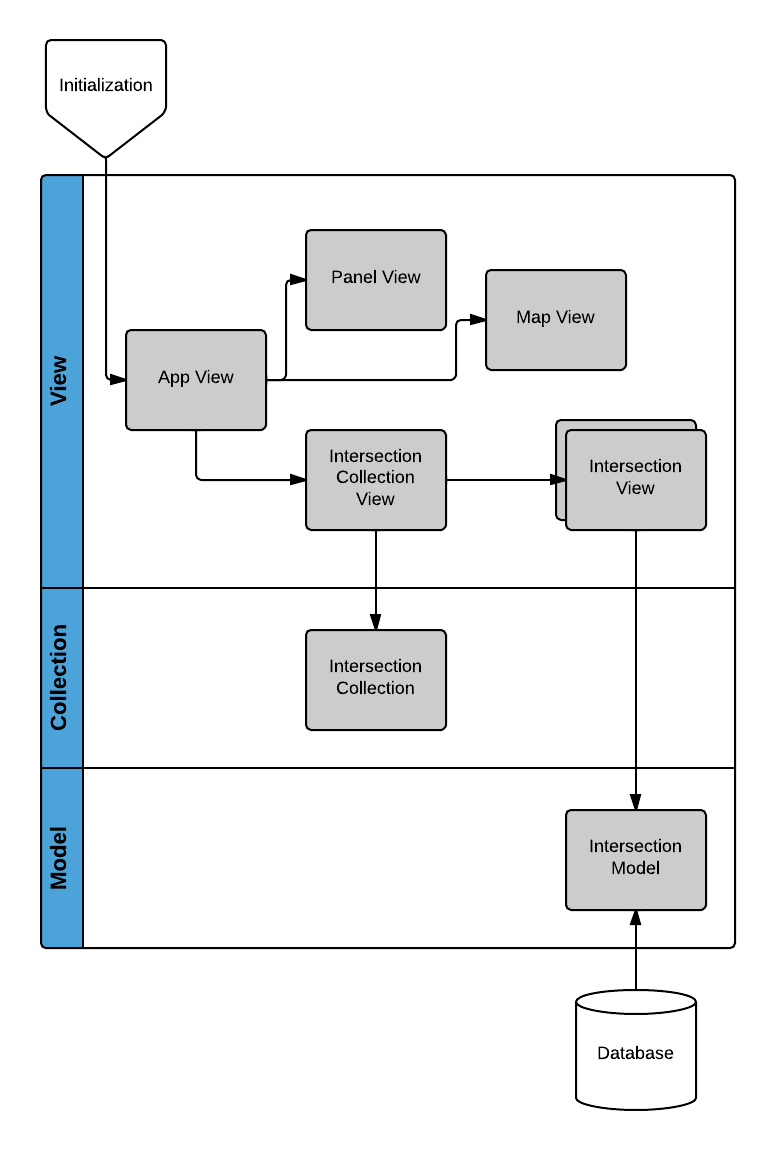
\includegraphics[scale=0.25]{figures/Iteration-2.png}
    \caption{An architectural diagram for Iteration 2.}
    \label{fig:iteration2}
  \end{centering}
\end{figure}

The third and final iteration of the architecture, as seen in figure \ref{fig:iteration3}, was developed for the final product demonstration and symposium.

The overall structure of the application is similar to that in the second iteration. The App View class is responsible for the high-level initialization and management of the application instance. The App View also owns both the main model collections and page views. The Road Model, Road Collection, and associated views were added to support the display of road information within the interface. Furthermore, three new pages were added in addition to the original map page view: Intersections Page View, Roads Page View, and Network Page View. These pages utilize the exiting data, yet present fundamentally different views and functionality around the data, supporting many of the non-crucial functional requirements. The addition of non-page and non-model views, such as the Panel View and the Activity View, encourage the application of Backbone's MV framework for the sake of uniform code patterning.

The value of storing one instance of the intersection and road collection objects is now clear, as the four pages now feed off of the same two data representations. This also means that all updating and synchronization of information between the client and server has been centralized, and thus the data is guaranteed to be consistent across the application.

\begin{figure}[htbp!]
  \begin{centering}
    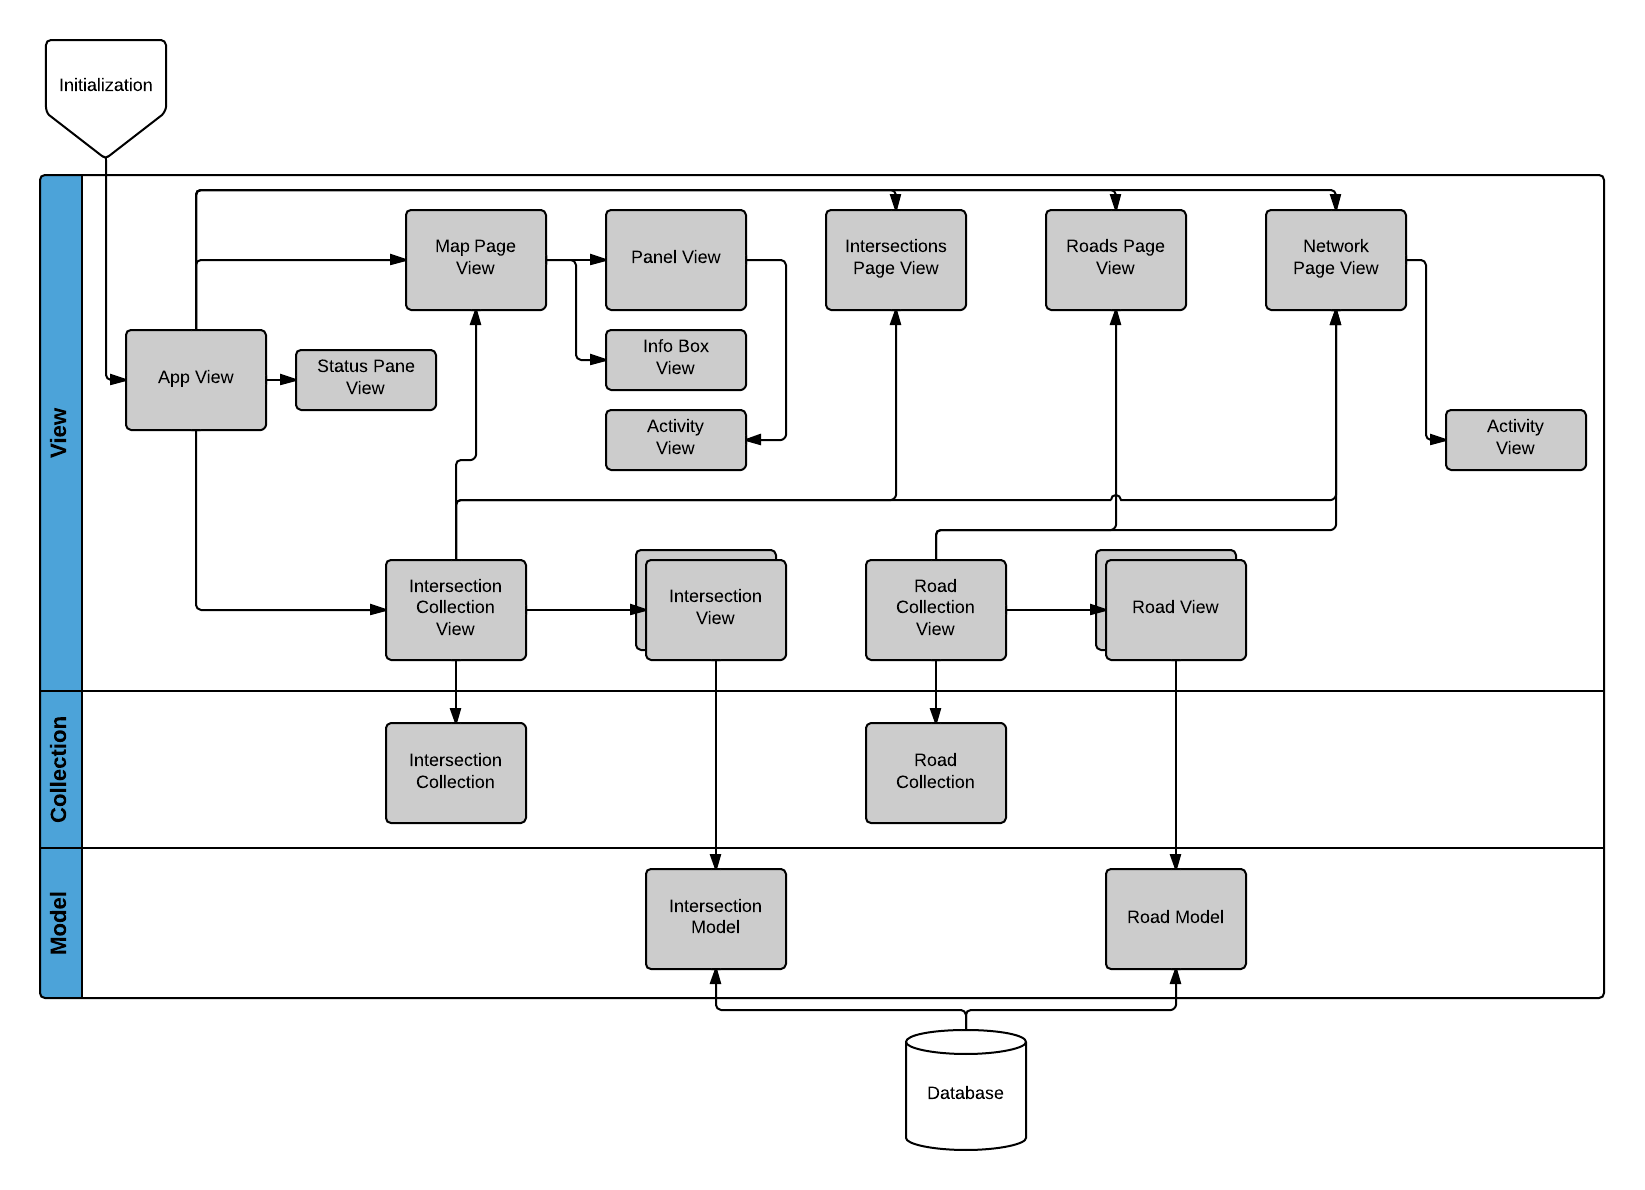
\includegraphics[scale=0.25]{figures/Iteration-3.png}
    \caption{An architectural diagram for Iteration 3.}
    \label{fig:iteration3}
  \end{centering}
\end{figure}

\section{Back End}
The infrastructure powering the user-facing component of Relay is colloquially referred to as the ``back-end''.
The design goal for this particular component consisted of providing all the necessary resources to the client-side application with minimal development effort (effort that would otherwise be spent on more innovative areas of development).
Additionally, this layer acts as the \emph{glue} that holds together the Relay system.
This is outlined at a high level in a full system map in Figure \ref{fig:Back_end_system_map}.
The back-end exposes APIs required for the client-side application (front-end), as well as data processing and scheduling routines for the Relay Framework.
This component is characterized by an application server, database, and associated services (such as map tiling).

The core application framework was chosen based on familiarity and flexibility (rather than performance).
For this task the ``Flask'' python framework was chosen, as many team members had worked in this environment successfully in previous projects.

\begin{figure}[H]
  \begin{centering}
    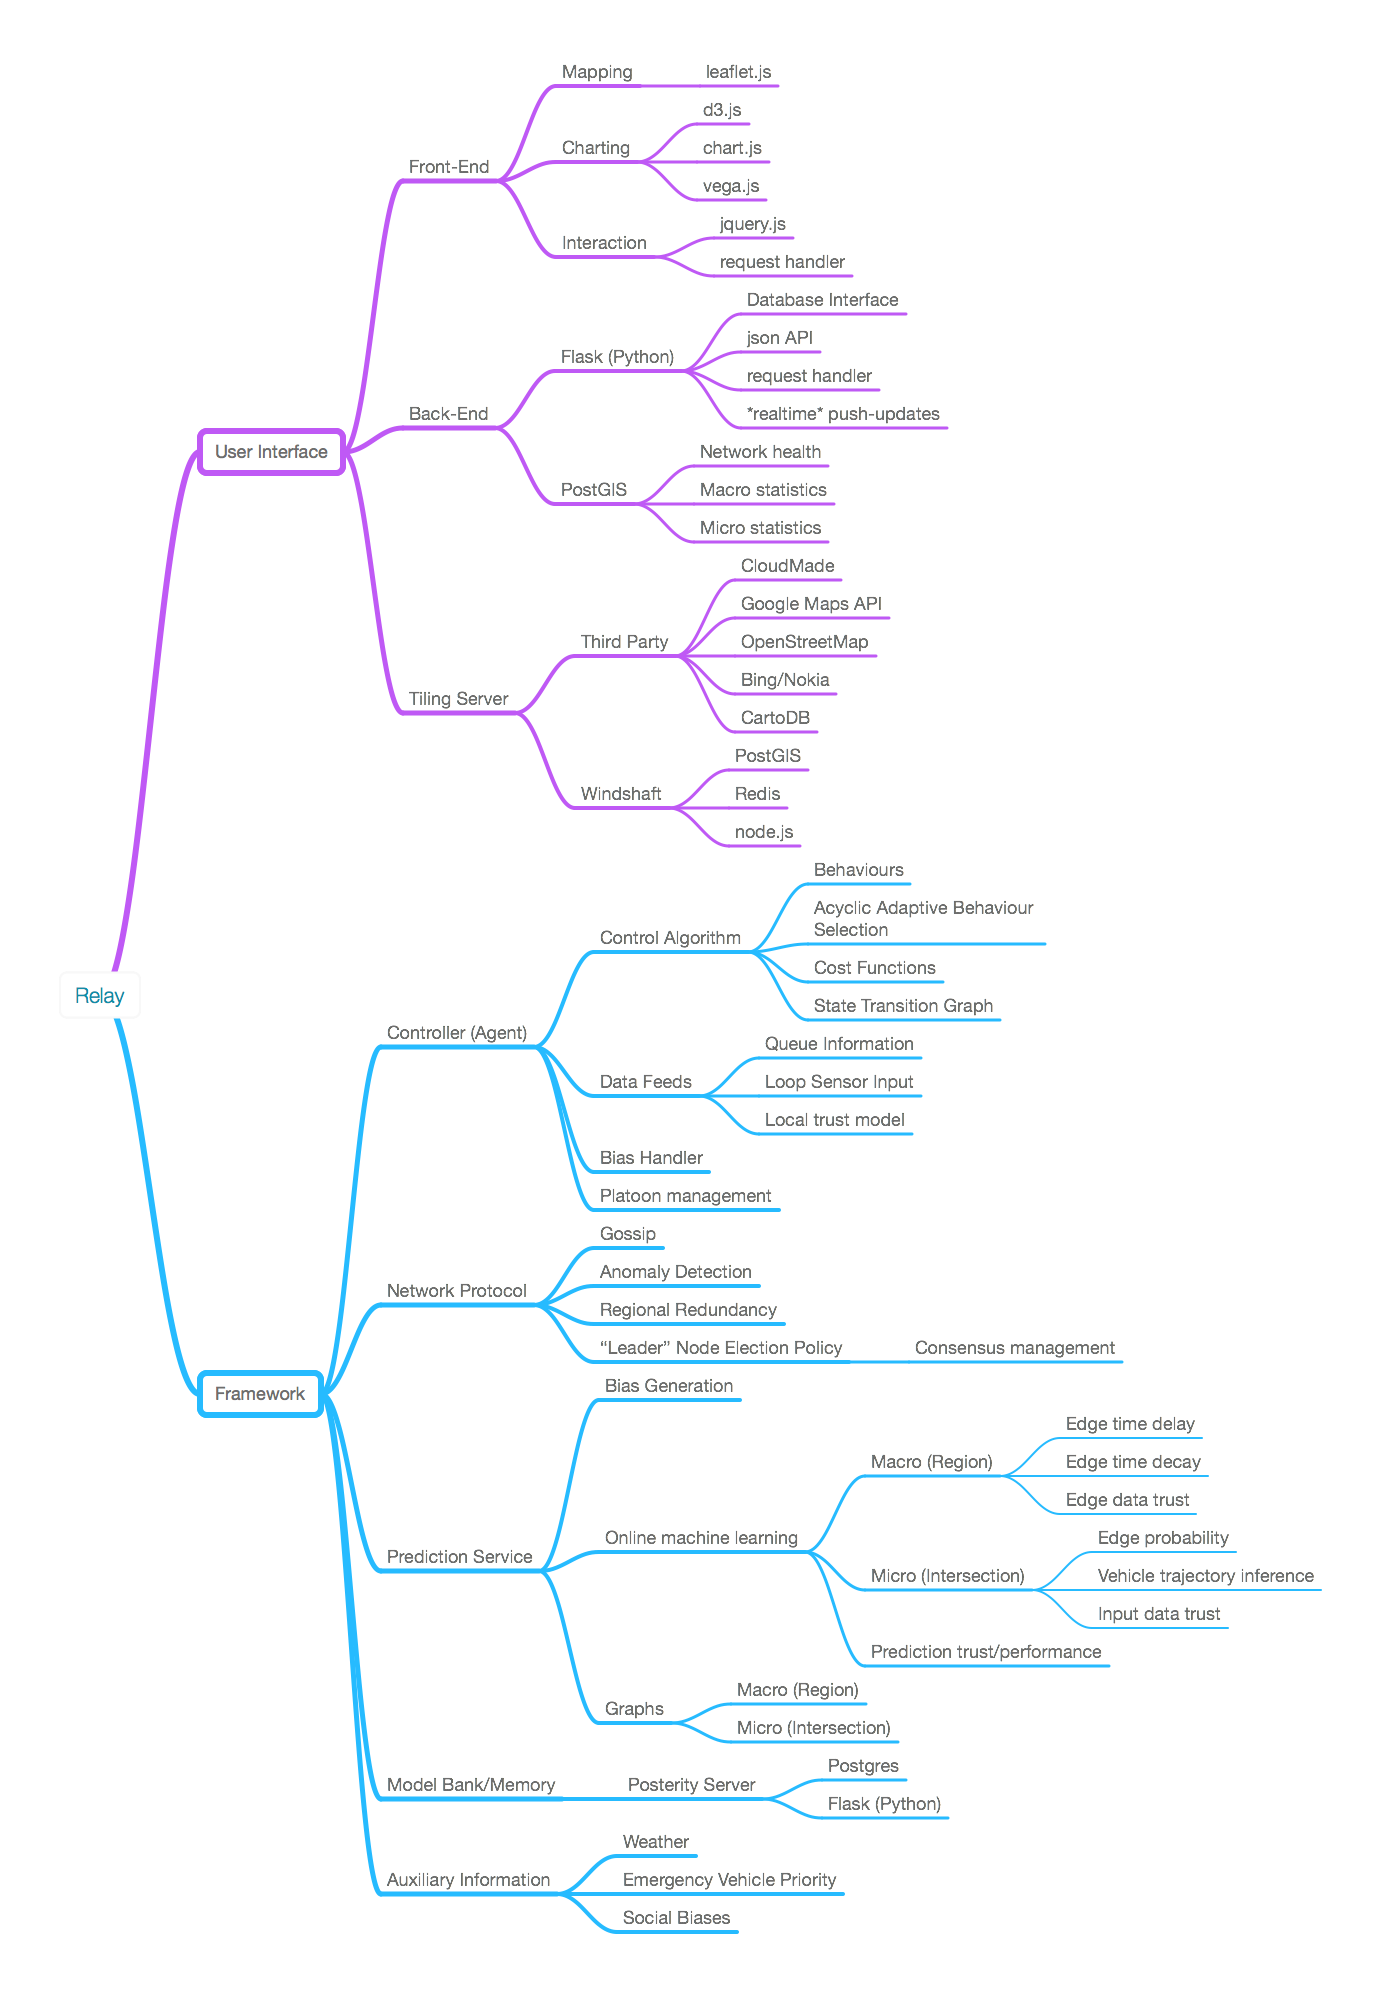
\includegraphics[scale=0.3]{figures/flow-chart.png}
    \caption{Relay: System Map}
    \label{fig:Back_end_system_map}
  \end{centering}
\end{figure}

Aside from the web-framework, the back-end design choices and technologies are broken up into modules.
To deliver the minimum viable product, the back-end must support online mapping via either a tile server or third party service, it must have some place to store various geospatial information (database), as well as some service to interface with the controller network (Relay Framework).
The various module design decisions and technologies selected are detailed below.

\subsection{Server - Flask and Python}
The Flask application acts a server with Relay passing information through the system to desired endpoints. This application contains functionality for transforming data, making network requests, serving information to front-end, and interacting with the database.

	Relay has multiple components and each works with the data in a specific format. Formatting is kept consistent throughout the system, using JSON formatted strings, but transformations are still required. The main transformation that needs to be performed is to change the time series data from the Erlang-server into information that can be better visualized on the front-end – explained in a <SECTION>.

	Network requests are defined by calls made to the Erlang-server, or “Framework”. The network contains all information regarding intersections, such as current behaviour, plans, and predictions. The Flask application is responsible for extracting this information and sending it to the database, front-end, or both.

	Lastly, the main function of the server is to accept requests from the front-end, process them, and serve the required information. Initially the majority of the information served comes from the database, but once the system is running, data is sent directly from the network to the front-end. This linkage is depicted in the system diagram, Figure \ref{fig:system-diagram}.

\subsection{Database - SQLite3}

As with most applications, the Relay web-service requires some medium to safely and efficiently store structured data, the canonical use case of a database.
Database technology is highly mature, and for its ease of use, familiarity, and extensive documentation, additionally, many members of the team are familiar with SQL.
To capitalize on this, a SQL relational database management system was chosen to power the Relay Interface.

SQLite3 was chosen as the database for its simplicity. 
These databases are contained entirely within a single file, and as such can be quickly and easily moved around the development environment (as well as captured by version control). 
The database contains information for: road metrics, intersection metrics, events, and Toronto's intersections and roads, acquired from their public data website <TORONTO>.

'Road metrics' stores the time delay parameters for each segment, along with a timestamp and associated node ids at the ends of the segment. 
'Intersection status' contains the current status of each intersection. 
In the case of 'failure' states at any intersection, explanations and further information would be found in 'Intersection events'. 
Intersection behaviours and plans are not contained within the database as of this iteration. 
In the future they could be added for historical lookups and use in planning, but for the purposes of the prototype this feature was not included. 
Tables have been created for these and could easily be integrated into the system.

\begin{figure}[H]
  \begin{centering}
    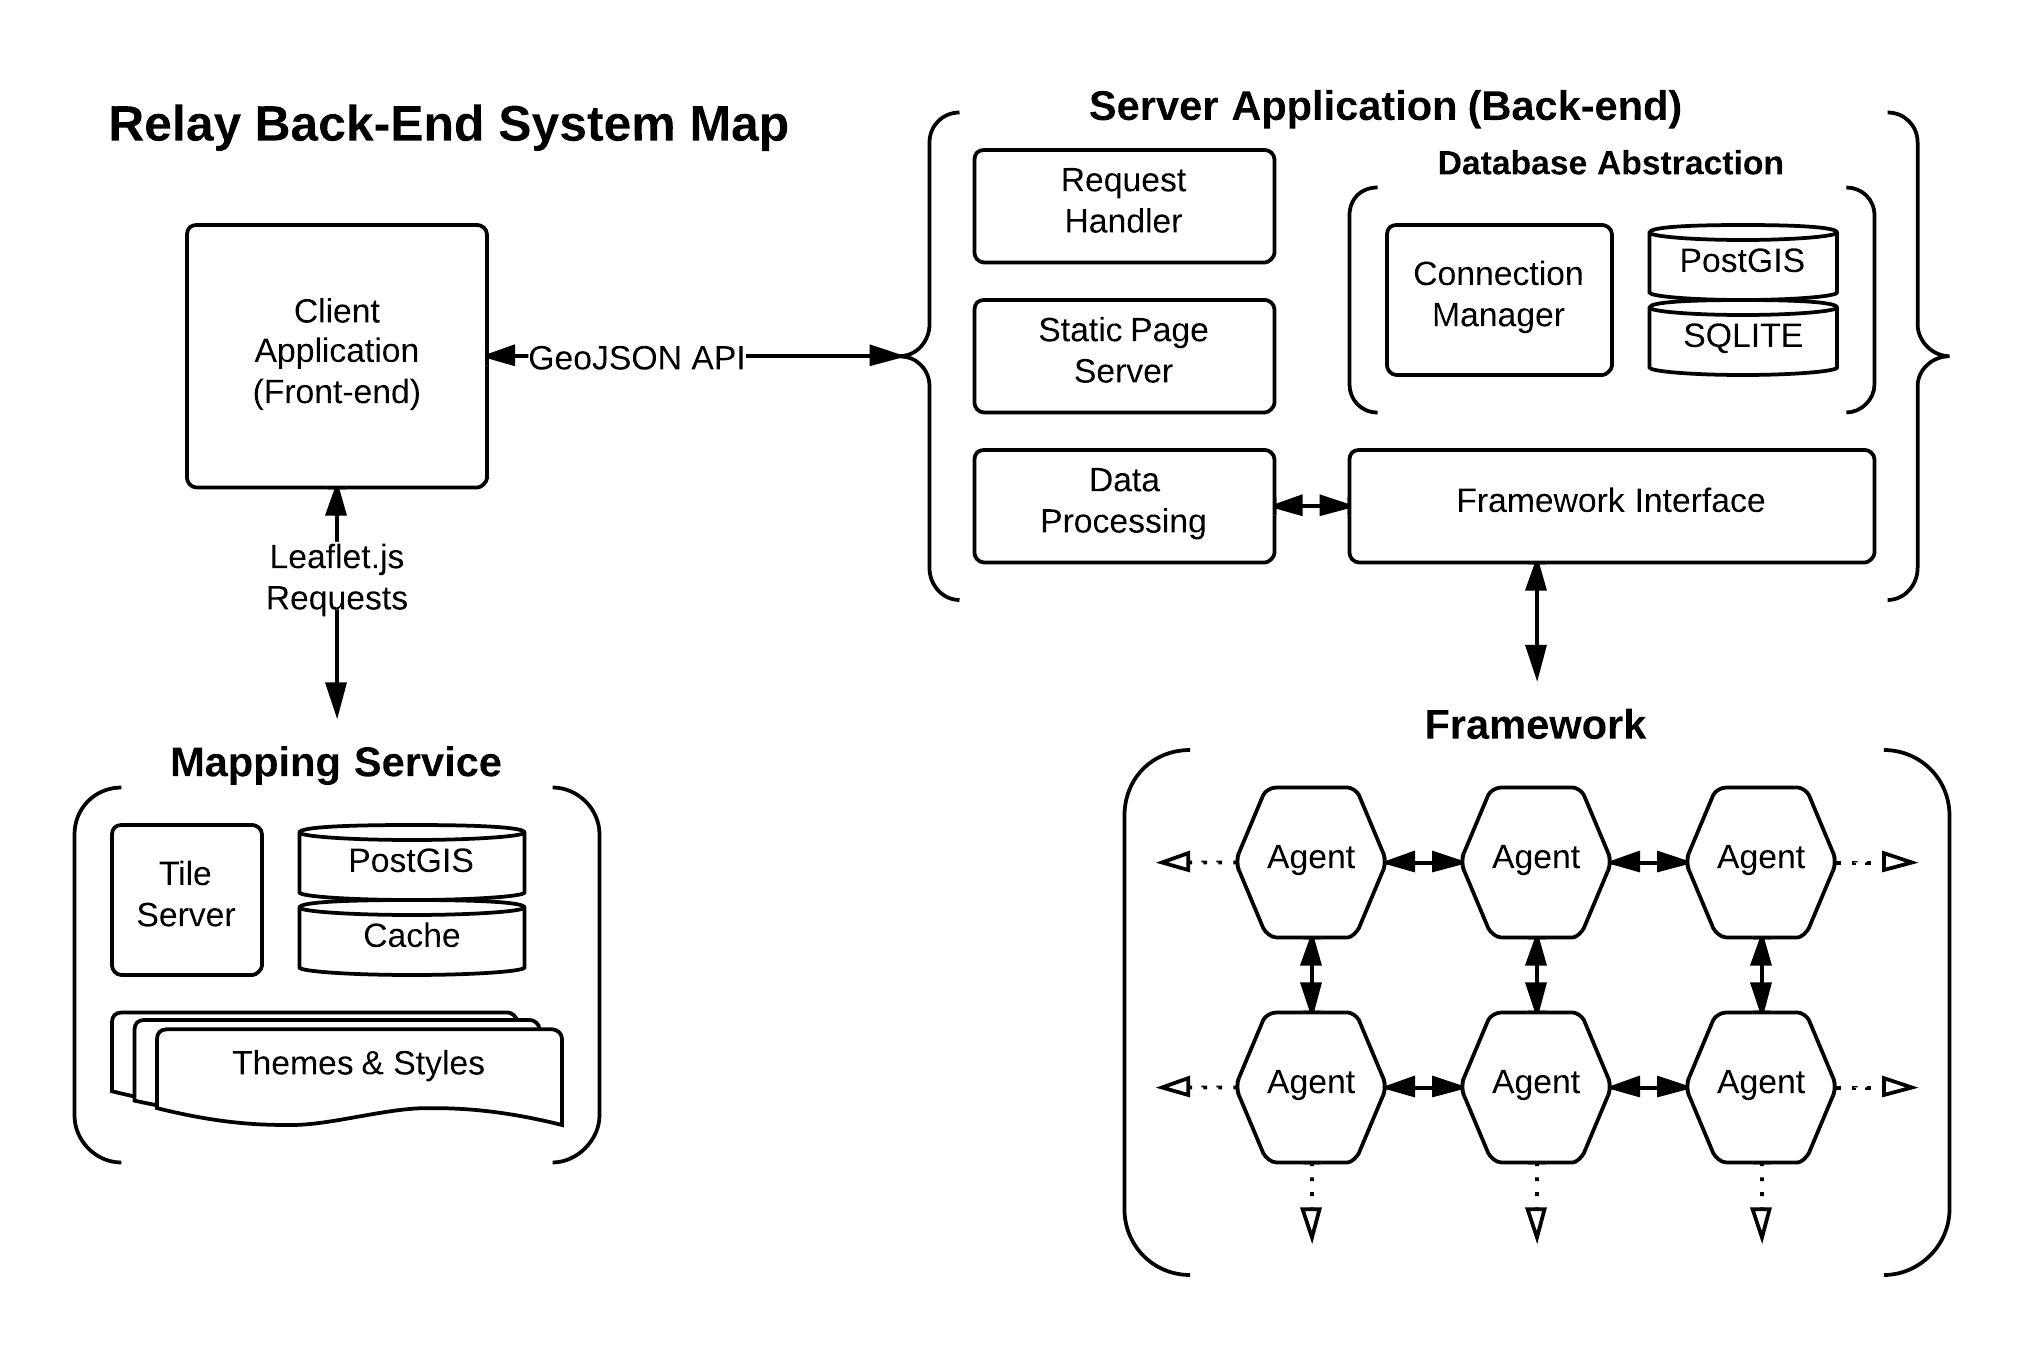
\includegraphics[scale=0.3,  angle=90]{figures/Relay_Backend_System_Diagram.png}
    \caption{Relay: Back-end System Diagram}
    \label{fig:system-diagram}
  \end{centering}
\end{figure}

\subsection{Client-Server Communication}
It is a goal of the solution to present up-to-date information about the network in the interface. This requires frequent communication between the client and the server. Client-server communication was achieved via the development of an Application Programming Interface (API) on the server, with which the client could connect to receive new information. The API was designed to specifically meet the needs of the solution, as API calls were designed specific features within the interface.

In order to maintain up-to-date information in the interface, the client was required to request new information from the API on a high-frequency schedule. Traditional HTTP requests require for the reload of a web page each time a request is made, so Ajax techniques were used in lieu of traditional HTTP requests. Ajax allows for asynchronous HTTP requests between the client and the server, which do not require the reload of the page upon completion. This successfully allowed for high frequency updates of the client without the negative performance implications of traditional HTTP calls.

\section{Deep End - Relay Framework}
\label{sec:deep_end}

Real-time, distributed traffic control is an interesting problem, with many creative solutions.
The modules and operators that handle individual intersection signal timing, data collection and backup, and statistical modelling, as well as the network topology that holds it all together is brought under the umbrella term ``Relay Framework'', in that the Relay Agent model can be used as a platform for developing more sophisticated agent-based traffic control suites.
The network of Relay Agents implementing the Framework are colloquilally referred to as ``The Deep End'' (as opposed to the typical application terminology of ``Front End'' and ``Back End'').

The ultimate goal of the Relay Framework (as defined mathematically in Section~\ref{sec:def:agent}) is to illustrate that complex chaotic systems (such as distributed acyclic traffic control) can become tractable within the context of a straightforward, symmetrical peer-to-peer architecture.
At the highest level, the loosely coordinated (read: not mesh) network of Relay \emph{Agents} tackles the traffic control problem through the intelligent use of local computation, rather than a single large-scale optimization problem to be undertaken sparsely at a centralised facility.
In isolation, each Relay Agent seeks to maximize intersection throughput (as measured through various arbitrary metrics) subject to local environmental/contextual constraints.
In concert, the Network achieves a sort of pseudo-temporal consensus, which itself acts as a stabilising factor on the decisions made by each agent.
In principle, the predictive consensus that is possible within the Relay Framework makes it \emph{easier} to achieve timing synchronisation between peers, despite not being a tightly coupled system.

We hypothesize that the added flexibility associated with such a scheme (i.e. being robust to failures, and reacting to anomalies) outweighs the potential cost associated with not having a centralised service.

This section is broken into 4 major components.
Section~\ref{sec:deep:motivation} is a high-level discussion surrounding the architectural design principles used in formulating the foundations for Relay.
Rationale for pursueing a sparsely connected peer-to-peer topology is presented, along with our approach for modelling uncertainty.
Section~\ref{sec:def:agent} defines the mathematical relationships and constructs central to the Relay Agent's design, including notions of predictive and regressive signals, graph transformations etc.
In section~\ref{sec:learning_in_relay} covers the manipulation of some of the design parameters central to the Agent's efficiency and performance, including reinforcement learning of delay kernels, and stochastic optimization procedures used to infer error in the underlying graph representation.
Section~\ref{sec:predictions_in_relay} covers the composition of the Agent's state parameters, with the delay kernels, illustrating how predictions are made and maintained by each Agent.
The chapter is concluded with the underlying optimization problem for scheduling the Agent's state transitions (Section~\ref{sec:opt:planning}), including predictive queue modelling.


\subsection{Architectural Motivation}
\label{sec:deep:motivation}

\subsubsection{Intersection Modelling}
\label{subsubsec:intersection_modelling}

Each intersection in Relay is modelled as a directed adjacency graph.
Wherein the nodes are represented as dual inlet/outlets (i.e. the incident edges represent the probability of flow \emph{to} the node, and emergent edges represent the probability \emph{from} the node.
A typical 4-inlet/outlet (symmetrical) intersection is shown in Figure~\ref{fig:intersection_graph}, wherein each ``node'' is broken out (by in/out-degree) into its constituent inlet/outlet.
\begin{figure}[!htpb]
	\caption{Example Intersection Graph}
	\label{fig:intersection_graph}
	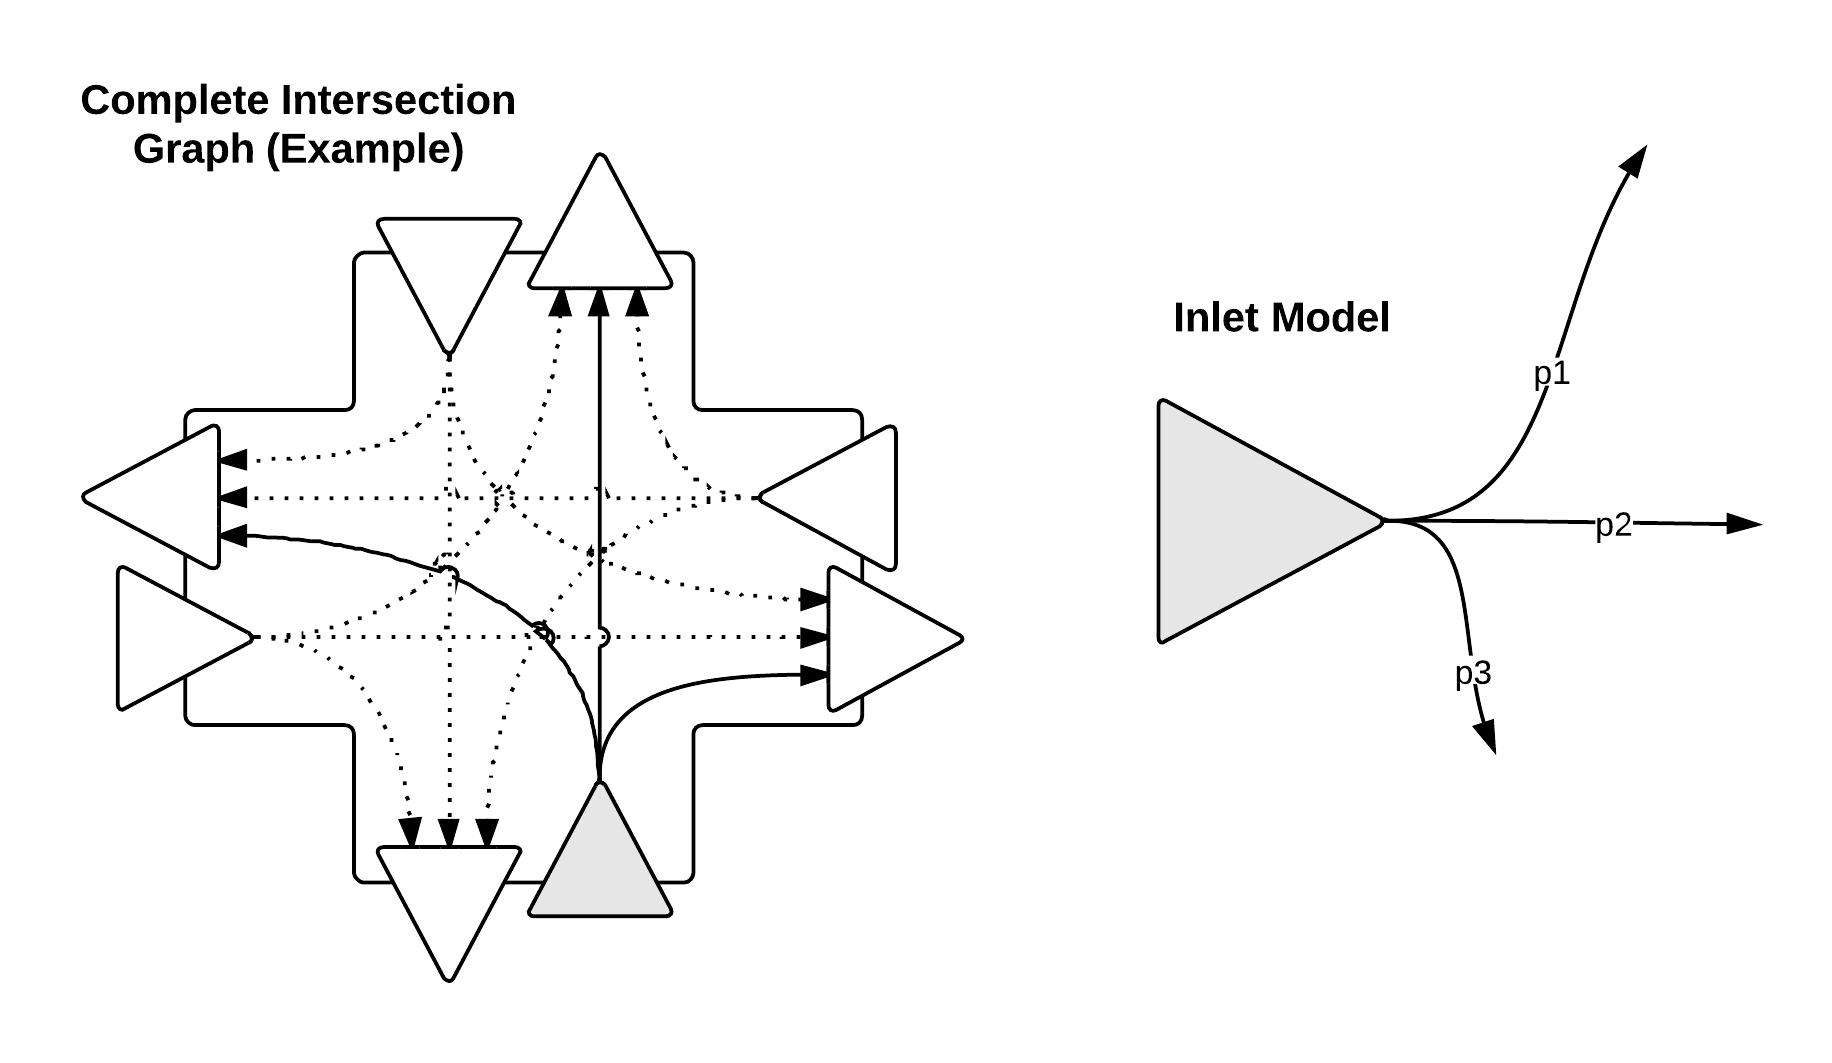
\includegraphics[width=\textwidth]{figures/Relay_Intersection_Graph.png}
\end{figure}

The concept of a generalized intersection within the Relay Framework is formalised in Section~\ref{sec:def:agent}.
This view of the intersection can be interpreted as an instantaneous probabilistic transfer function: given that a vehicle enters an inlet, the emergent edges from that inlet represent the probabhility that the vehicle will \emph{emerge} at the prescribed outlet.
This probabilistic view of \emph{traffic as a wave} is found throughout the Framework, and forms the basis for many of the probabilistic signals used throughout.


\subsubsection{A Peer-to-Peer Solution}
\label{sec:p2p_philosophy}

Relay was designed to be a distributed system, both in the computer-science sense of the word, as well as the geographical sense.
The advantages associated with a geographically distributed system are revolve around the reduction in concentration risk---for example, given a regional power-outage, or natural disaster the liklyhood that the entire network is affected is low if it is distributed across a large region.
This of course comes at the cost of added complexity in agent design (i.e. in a typical peer-to-peer sense, each Agent becomes simultanously a client and server), as well as increasing the relative scarcity of inter-agent communication bandwidth.
The underlying philosophy of the Relay Agent design is to mitigate these two constraints, while exaggerating the benefits associated with distribution.

This design breaks with the traditional centralised (or recently, ``Cloud Based'') approach to traffic synchronisation, which is used extensively by modern installations (i.e. the ranks of which include Miovision's Spectrum).

\paragraph{Communication: Making Every Message Count}
Relay Agents communicate a lot; their prediction feeds, their sensor feeds, etc.
Thus is is infeasible for all Agents to be densely connected, as the system as a whole would be bogged down with network chatter.
This constraint is addressed in two main components, the first of which is a explicit restriction on the connectivity of the Agents.
As shown in Figure~\ref{fig:Relay_Network}, each Agent is only connected to its immediate peers (with suplementary connections made available on-demand---such as for system upgrades etc.).
Thus the network that each agent \emph{sees} looks like a full mesh centered around it.
This virtually eliminates poor scaling behaviour for large networks, and alleviates the associated computational burden associated with high-volume network traffic.

\begin{figure}[!htpb]
	\caption{Relay Network Neighbourhood}
	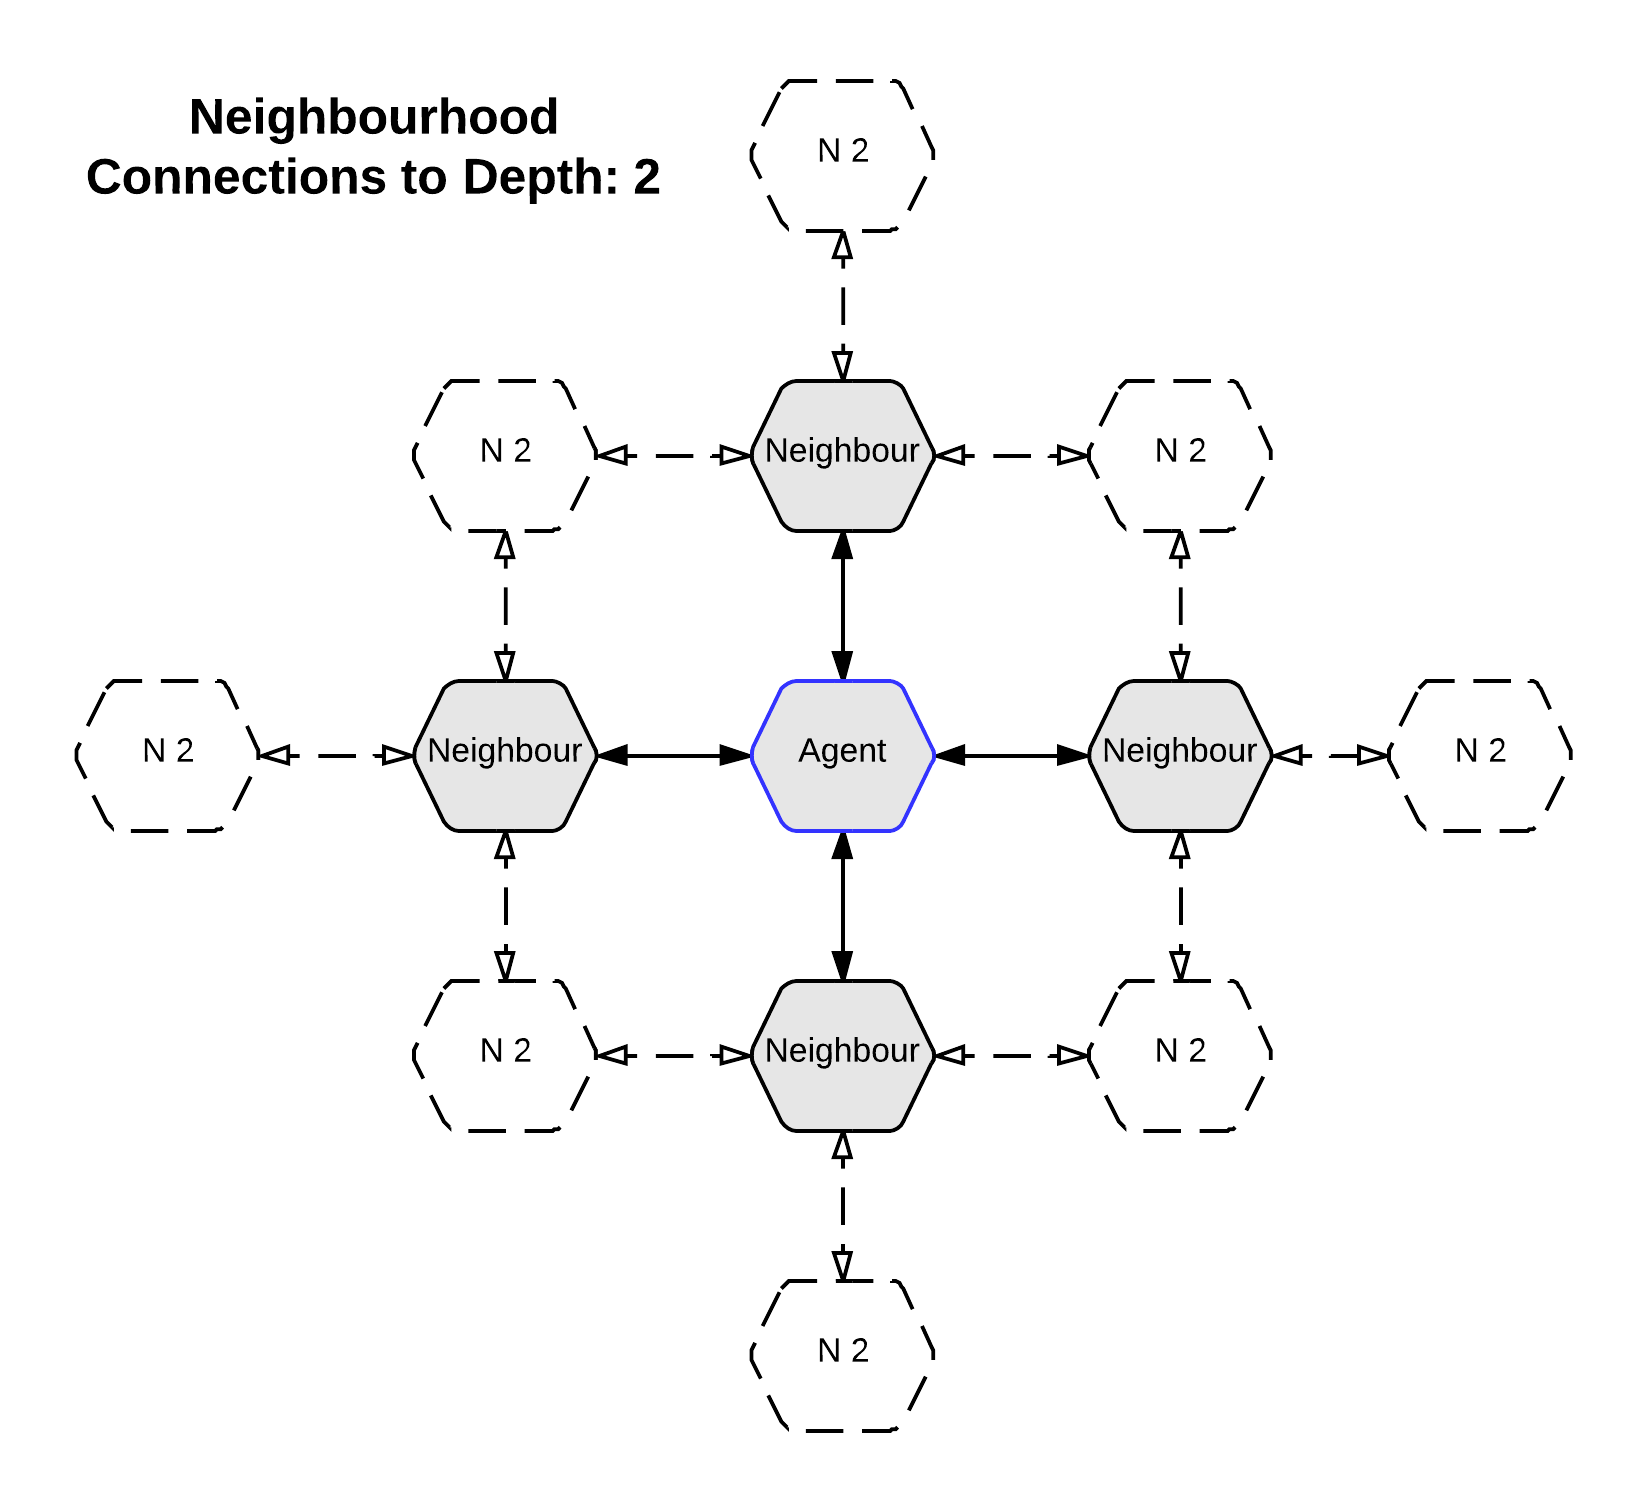
\includegraphics[width=\textwidth]{figures/Relay_Network.png}
	\label{fig:Relay_Network}
\end{figure}

However this puts additional constraints on the type of the information that can be communicated, and Agent can't (directly) inform its neighbour 3-intersections downstream of an incoming platoon, this information must be transformed and \emph{relayed} through the network.

\paragraph{Dense Signals}
As alluded to above, the network connectivity restrictions placed on the Relay network imply a severly reduced view of the traffic environment as a whole.
In Relay, agent's get around this through explicit use of statistical projections/predictions of traffic flow.
Their own internal schedules feed back into these predictions, and the predictions themselves propagate through the network, with each step in the propagation, each Agent modifies it with their own predictions.

In essence, when one vehicle enters (stimulates) a connected inlet, the vehicle is no longer considered as a discrete event, but rather a probability wave. 
In isolation, each Agent in the \emph{expected} path adjusts their behaviour schedules to allign with the expectation.
Once the adjustment calculation is complete (which in an indeal world is instantaneously), the Agent then propagates a modified wave to its peers, and so on.

\paragraph{Leveraging Asynchronous Distributed Computation}
In an abstract convergent sense, the network alligns itself to the most likely routes that this hypothetical vehicle would take.
In essense, we \emph{cheat} the connectivity problem, by infusing each message with as much computation as is reasonable (after all, prediction is in general computationally expensive), this acts as a form of compression, albeit in terms of \emph{work}, the actual messages sent `over the wire' could also be compressed as well---but thats an implementation problem.

If we take a snapshot of an Agent in time, we would expect to find a large amount of information that represents not just the local environment, but somthing that reflects the superposition of many peer's views of the network.
In a sense, by examining the state of a given Agent, we can infer the traffic environment around it with great detail (essentially the resolution is temporal rather than spatial).

\subsubsection{Modelling Uncertainty}
\label{sec:modelling_uncertainty}

One of the most significant hurdles for any predictive component is the concept of uncertainty.
As evidenced by the (relative) success of traffic control systems in general, traffic can be in many circumstances deterministically modelled (especially in the case of fixed-timing networks, wherein the traffic is whatever you decree it should be, regardless of whether that is `optimal').
In Relay, there are two principal probabilistic models, the first is the intersection transition graph (as described in Section~\ref{subsubsec:intersection_modelling}, and formalised in Section~\ref{sec:def:intersection_graph}), which models the liklyhood that a vehicle will take a particular action at an intersection.
This is used as the basis for transforming discrete \emph{real} traffic signals (derived from physical measurements) to expectation signals, as well as for the optimization associated with the signal timing.

The second of which is the delay kernel, which is ultimately a statistically learned parameter which is formalised in Section~\ref{sec:def:expected_ingress}, in the context of informing predictions.
This way in which this parameter is learned is further described in Section~\ref{sec:learning_in_relay}.




%%  THE RELAY AGENT  %%%%%%%%%%%%%%%%%%%%%%%%%%%%%%%%%%%%%%%%%%%%%%%%%%%%%%%%%%%%%%%%%%%%%%%%%%%%%%%
\subsection{The Relay Agent}
\label{sec:def:agent}

At its heart, Relay is a \emph{dynamic graph automata}, whose state changes (the most visible of which is the underlying traffic light values) are based on a combination of inputs from the environment, and its immediate neighbors in the Relay network.
Each traffic controller in Relay is an autonomous \emph{Agent}, that (as the network deepens/expands) forms transient, asynchronous communication channels to its neighbors.
This section will formally describe and define the underlying mathematical constructs used to implement the various aspects of the controller, as well as the various inputs and outputs of the system.


\subsubsection{Intersection Graph}
\label{sec:def:intersection_graph}

The intersection is represented as the graph $\bf{G}^{n \times n}$ defined in equation~\eqref{eq:def:base_graph}, whose $n$-nodes are the inlets/outlets of the intersection.
The edges $\bf{G}_{ij}$ indicate the probability that an ingress event (or idealized vehicle) at node $i$ will instantaneously exit the intersection at node $j$, which is formalized in~\eqref{eq:def:internal_probabilities}.

\begin{equation}\label{eq:def:internal_probabilities}
	G_{ij} = p\left(\bf{G}_i \mapsto \bf{G}_j \right) = p_{ij}
\end{equation}

\begin{equation}\label{eq:def:base_graph}
	\left[\bf{G}\right]_{n \times n} =
	\left(
		\begin{array}{ccc}
			p_{11} & \cdots & p_{1n} \\
			\vdots & \ddots & \vdots \\
			p_{n1} & \cdots & p_{nn}
		\end{array}
	\right)
\end{equation}

$G$ has some notable properties that allow for some algebraic simplifications, the most significant of which is that there can only be one edge connecting node $i$ to node $j$, and that we can treat it as a undirected adjacency graph, making it trivial to express it efficiently as a matrix.
The $p_{ij}$ notation is used to indicate that the underlying edges represent probabilities rather than length or weights.
It is thus the case that the sum of all exit probabilities associated with a given inlet is always 1, this is formalized in~\eqref{eq:probability_sum}.

\begin{equation}\label{eq:probability_sum}
	\sum_{j=1}^n p_{ij} = 1 \; \forall i \in \left[1, n\right]
\end{equation}


\subsubsection{Agent Behavior}
\label{sec:def:behaviors}

If the goal of these structures is to describe the Agent's representation of the state of the intersection it controls, then $\bf{G}$ is insufficient---after all, taken at face value, $\bf{G}$ implies that if two vehicles are incident at the same time, they both instantaneously \emph{diffuse} to their expected outlets, without any sort of interaction.
Real intersections don't do this, and real vehicles are not waves (despite how much it would help traffic control).
The entire concept of a `Red Light' is to avoid the superposition of vehicles in space and time.

In Relay, the concept of a particular set of `active' or `Green' lights (canonically termed a ``phase'') are encapsulated in the \emph{Behavior} construct.
Behaviors in Relay control the \emph{visible} intersection transition graph of the intersection, by operating on the values of particular edges.
In essence, setting a particular edge probability to zero, means that vehicles cannot transition through the edge; limiting the throughput of the intersection (kind of like a traffic light).

Formally, behaviors in relay are elementwise masks on $\bf{G}$, each of which is a member of the finite set $\bf{B}$ as shown in equation~\eqref{eq:def:behaviors}.

\begin{equation}\label{eq:def:behaviors}
	B_{ij} \in [0, 1] \; \forall B \in \bf{B}
\end{equation}.

Note that while we have defined the range of acceptable values for $B_{ij}$, we exclusively set each $B_{ij}$ to either 0, or 1 representing ``off'' and ``on'' respectively.
Ultimately, the most important property of the Behavior, is that in composition with $\bf{G}$ it forms what we'll hereafter refer to the ``visible'' intersection graph, or rather the physically realizable transfer graph of the intersection.
The visible graph $\bf{V}_k$ is thus defined in equation~\eqref{eq:def:visible_graph}.

\begin{equation}\label{eq:def:visible_graph}
	\left[V_k\right]_{n,n} = \left[B_k\right]_{n,n} \circ \left[\bf{G}\right]_{n,n}
\end{equation}
where $B_k$ is the $k^{th}$-member of the set of behaviors $\bf{B}$, and ``$X \circ Y$'' is the elementwise/Hadamard product of matrices $X$ and $Y$ (which must have the same shape).


\subsubsection{Ingress Signals}
\label{sec:def:ingress}

While not sufficiently defined, the Relay agent as a single unit is a dynamic system with many vector outputs.
As implemented however, the system only gathers input from a single source: incidence---or ingress events.
Physically, these can be thought of as discrete events triggered by physical sensors installed at the inlets of the intersection, such as the quintessential inductance/loop sensor frequently found near controlled intersections.
Internally, Relay is agnostic to the type of sensor (and associated preprocessing necessary to transform raw sensor input into an ingress event) used in the network.

At its core, the incidence signal is interpreted as a record that a vehicle (or arbitrary client of the intersection) has entered the intersection.
The incidence $a_i$ at the $i^{th}$ inlet of $\bf{G}$ is a combination of two measurements: the \emph{weight} of the arrival (interpreted as how significant the ingress is, i.e.\ a bus or truck could be considered `larger' than a single vehicle or bicycle), and the time the event happened.
These records (weight + time pairs) are combined into the ingress \emph{signal} associated with a particular node of $\bf{G}$, and concatenated together to form the vector-valued signal $\vec{a}(t)$ whose elements are defined in equation~\eqref{eq:def:ingress}.

\begin{equation}\label{eq:def:ingress}
	a_i(t) = \sum_{k \in A_i} \omega_k \delta(t - \tau_k)
\end{equation}
where $A_i$ (in the idealized representation) is the set of ingress events $\{(\omega, \tau)\ : \tau \in [-\infty, t]\}$, or rather, the set of all ingress events that have been observed at the $i^{th}$-node.


\subsubsection{Egress Signals}
\label{sec:def:egress}

As previously described, the incidence signals represent the core \emph{real} measurements that are used by the agent.
While immediate ingress information is necessary in that it is physically where the sensors for a particular intersection are often located, in their current state they are not useful signals for controlling the intersection behaviors/state transition (which is the reason for collecting the information to begin with).

The motivation for performing a transformation on this data is further increased when we recall that Relay agents are designed to communicate with one another.

Lets get the analogies rolling: If the operator of a train station wanted to plan for serving the people exiting the trains stopping at her station, and that the preparations for a train stopping took 15-minutes.
The knowledge that there was currently a train stopped at her station is not valuable for planning, and as such, if that was the only knowledge she had she would be unable to plan.
Of greater value, would be the knowledge that there was currently a train inbound from some connecting station.
This---combined with some prior information about roughly how long it took trains to cross the distance between the two stations, would allow her to better time the preparations.

This ``incoming'' signal is essentially a special case of what we term a \emph{remote egress signal}.
Relay Agents ``upstream'' will inform their ``downstream'' peers of vehicles \emph{leaving} their intersection.
Taken from the perspective of a single agent, this means that the ingress signal should be transformed to an associated \emph{egress} signal.

Using the definitions in equations~\eqref{eq:def:visible_graph}, and~\eqref{eq:def:ingress}, we can define the egress signal as a linear transformation of the ingress signal, by the agent's visible graph $V$.

\begin{equation}\label{eq:def:egress}
	e_j(t) = \sum_{i=1}^n a_i(t) V_{ij}(t)
\end{equation}
Note that we have additionally indicated that the agent's visible graph is time-varying, this is helpful in simplifying the description of these signals, but ultimately doesn't reflect the physical reality of signal timing.
Intuitively, we would expect that the agent's visible graph would change in discrete `jumps'.
This is not far from the truth, and exposes the beating heart of the relay agent.


\subsubsection{Behavior Transition}
\label{sec:btg}

As alluded to above, what makes signal timing control challenging is not inherently that there is a vast continuum of misinformation and environmental variability (although that certainly doesn't help the problem), but rather that we have a finite set of ``solutions'' or ``strategies'' to employ, and pesky physical restrictions (why can't all the lights be green all the time?).

In equation~\eqref{eq:def:behaviors}, we referred to a set of behaviors $\bf{B}$, and in equation~\eqref{eq:def:egress} we referred to the time-varying graph $V(t)$.
In order to define \emph{how} the visible graph changes over time (as a result of behaviors switching) we now introduce the concept of ``Behavior Transition'' in equation~\eqref{eq:def:btg}, whose edges are the incurred time-cost associated with a given behaviors transition (i.e. ``Yellow''-time between ``Green'' and ``Red'' states) as defined in equation~\eqref{eq:def:btg_costs}.

\begin{equation}\label{eq:def:btg_costs}
	\Tau = \{\mbox{cost}\left(B_i \mapsto B_j \right) : \forall B_i, B_j \in \bf{B} \}
\end{equation}
Where it should be noted that we have freedom to define an arbitrary transition cost function.
Within the Relay implementation we have frequently used time-values corresponding to the legally mandated ``yellow'' time associated with transitions to ``Red'' (on the order of 2-seconds), or the dead-time associated with transitions from the ``Red'' behaviors.

\begin{equation}\label{eq:def:btg}
	\bf{\Gamma} = G(\bf{B}, \Tau)
\end{equation}

Thus we define the Behavior Transition Graph $\Gamma$, as a directed graph whose nodes are behaviors (members of $\bf{B}$) and whose edges are the associated costs for transitions between adjacent behaviors.


\subsubsection{Ingress Expectation}
\label{sec:def:expected_ingress}

In Section~\ref{sec:def:egress} we expressed that the egress signal of an agent's peer is only valuable in conjunction with some expectation of how long the signal will be delayed.
For example, if we know that on average the train will take 20-minutes to travel from the neighboring train station to the local one, we can  generate an expected arrival time for the train.
In Relay, this expectation is generalized to include arbitrary delay-\emph{kernels}.

Recall in Section~\ref{sec:def:ingress} that we generated an ingress signal based purely on local measurements.
The Agents in Relay also generate an \emph{expected ingress} signal $E\left[a_i(t)\right]$ as defined in equation~\eqref{eq:def:expected_ingress}.

\begin{equation}\label{eq:def:expected_ingress}
	E\left[a_i\right](t) = \sum_{j} \left(e_j^{nbr}(t) + E\left[e_j^{nbr}\right](t) \right) * h_{ji}(t)
\end{equation}
where $e_j^{nbr}(t)$ is the egress signal (as defined in equation~\eqref{eq:def:egress}) of the neighboring agent that is upstream of the $i^{th}$ inlet of the local agent, and $E\left[ \cdot \right]$ denotes the expected value.
Note that by including a summation over $j$ there can be multiple upstream signals that can be combined to generate this expectation.
Further note the inclusion of the expected upstream egress signal---the derivation of which can be found in equation~\eqref{eq:def:expected_egress}.
Further note that the choice of delay kernel $h(\tau)$ is left entirely to the implementation.
In the Relay prototype, these took the form of Gamma distributions, whose parameters were tuned via reinforcement learning.

\subsubsection{Egress Expectation}
\label{sec:def:expected_egress}

In Section~\ref{sec:def:expected_ingress} we formulated the expected ingress signal in terms of a delay kernel $h(\tau)$ and a superposition of signals from a neighboring agent---explicitly relying on inter-agent communication, and prior knowledge of the particular delay distribution between the connected agents.

In a similar fashion, the expectation of the local egress signal follows a similar flow, albeit with a subtle variation.
In equation~\eqref{eq:def:expected_ingress} the expected ingress was formed (in part) from a signal derived exclusively from real measurements; namely $e^{nbr}_j(t)$---a neighbor's egress signal, which via equation~\eqref{eq:def:egress} was directly derived from real measurements (incidence signals).

An agent's expected egress is co-recursively defined in terms of its expected ingress in equation~\eqref{eq:def:expected_egress} which is simply a repetition of equation~\eqref{eq:def:egress}, utilizing the linearity of the expectation operator.


\begin{align}\label{eq:def:expected_egress}
	E\left[e_j\right(t)] &= \sum_{i=1}^n E\left[a_i V_{ij}\right(t)]\\
						&= \sum_{i=1}^n E\left[a_i\right](t) E\left[V_{ij}\right](t) + \mbox{Cov}(a_i(t), V_{ij}(t))\\
						&\approx \sum_{i=1}^n  E\left[a_i\right](t) E\left[V_{ij}\right](t)
\end{align}
In equation~\eqref{eq:def:expected_egress} the Covariance of the two time-signals is assumed to be near zero, however it is important to understand the cases where such approximations may introduce large error into the system.
The first of these is predictive feedback.
Due to the corecursive definition of the expected egress and ingress, the results from one calculation can propagate through a closed loop of peers, thus becoming correlated to the other.

The second relies on the transition plan associated with the agent, which is remains constant over a relatively short timescale, and directly controls $V_{ij}(t)$, and thus the expected egress of an agent.
In general, it is hypothesized that for loosely-coupled networks (characterized by having delay kernels with large average delays) this is a nonissue.
For tightly coupled networks, care should be taken incorporating prediction values in the optimization routine chosen to generate plans.
However, it may be the case that in the \emph{real} world, it is unlikely that individual participants would exhibit geographically cyclic behaviors exaggerated enough to damage the validity of the expected egress prediction (i.e.\ driving in circles).
To add even greater ambiguity, we hypothesize that the introduction of bias due to the assumption of statistical independence may actually increase performance in tightly coupled networks (i.e.\ by implicitly biasing agent's timing in favor of things with cyclic behaviors, such as public transport and logistic vehicles).

\subsubsection{Acyclic Scheduling}
\label{seq:def:plan}

In a sense, the final piece of the Relay Agent puzzle; the Agent internally stores a \emph{plan} that governs when, and to which behaviors the agent will transition over some future time window.
The ``Behavior Transition Plan'' (BTP, or simply ``plan'') is the combination of a particular \emph{path} through the behaviors transition graph (defined in equation~\eqref{eq:def:btg}) with the times associated with each step in the path.
Given a plan, it is thus possible to generate the visible graph signal $\bf{V}(t)$, and via a behaviors lookup-table, this process is invertible.
The plan---and its properties, are defined in equations~\eqref{eq:def:plan}.

\begin{align}\label{eq:def:plan}
	\mbox{plan} = \{(B_i, t_i) : t_{i} &\geq t_{i-1} + \Gamma_{B_{i-1},B_i},\\
	B_i &\in \mbox{Adj}_\Gamma(B_{i-1}) \forall B_i \in \bf{B}\\
	\forall i &\in [0, d]\}
\end{align}

Which is to say, that each successive step in the plan must take place after the current step plus the cost of taking the step (as formalized in equation~\eqref{eq:def:btg}), and that each successive behaviors, must be adjacent-reachable in $\Gamma$.
Additionally, the length of the sequence is limited to some finite integer $d$, which corresponds to the \emph{depth} of the path (or length).

In equation~\eqref{eq:def:behavior_signal} we define how the plan defines the behavior signal.
Given this description of a path, it is trivial to connect this representation to the visible graph signal $\bf{V}(t)$ as defined in equation~\eqref{eq:def:visible_graph}.

\begin{equation}\label{eq:def:behavior_signal}
	B(t) = \sum_{k=1}^{d-1} (u(t - t_{k-1}) - u(t - t_k)) B_k, \; (B_k, t_k) \in \; \mbox{plan}
\end{equation}
Where $u(\tau)$ is the Heaviside/unit-step function defined in equation~\eqref{eq:def:u}
\begin{equation}\label{eq:def:u}
	u(\tau) = \left\{
		\begin{array}{lr}
			1 & : \tau \geq 0\\
			0 & : \tau < 0
		\end{array}
		\right.
	\end{equation}
It is through manipulations of $\Gamma$ that the agent is able to consider various behaviors, as well as limit the acyclic behaviors associated with a \emph{plan} to legal states (for both real-world and abstract definitions of ``Legal'').

%%  LEARNING IN RELAY  %%%%%%%%%%%%%%%%%%%%%%%%%%%%%%%%%%%%%%%%%%%%%%%%%%%%%%%%%%%%%%%%%%%%%%%%%%%%%%%%
\subsection{Learning in Relay}
\label{sec:learning_in_relay}

Each agent within the system has multiple design parameters that will constantly update. With each cycle -- behaviour change -- predictions and estimations are made to recalculate these parameters. 
The following sections explain how these variables are learned and updated.

\subsubsection{Time Delay Estimation}

The first important parameter needed to calculate predictions is the time delay estimate between two agents. 
This can be thought of as the estimated time to travel from one intersection to a neighbouring one. 
However, this is not a fixed time, so the delay is modelled using a gamma distribution, as discussed previously. 

The first step in performing this estimation, is determining which portion of the downstream signal is relevant – meaning what part of the signal should be considered for the estimation. 
This is required because it must match the departing signal from the upstream intersection. 
To extract the downstream signal, an upstream sub-signal is first selected. It was determined that the most efficient way to do this is to this is to select the upstream departure signal created by the previous behaviour cycle. 
To ensure that events are not missed, the downstream signal is determined by time-shifting the upstream signal by the expected value of the previous time delay distribution, and a small buffer is added to each end.

After the two signals are extracted, the estimation process can be performed. 
Equation [time-delay-opt] outlines the optimization problem, using least squares. 
The goal of this optimization is to convolve the departure signal with a gamma distribution to best estimate the downstream arrival signal -- to minimize the difference between the real signal and estimated. 
The design parameters are: shape, location, scale, and gain. 
The first three are what control the parameters of the distribution and the last is a measure of the change in cars while traversing the road -- to capture the effect of cars turning onto or off of the road on side streets.

Below, in Figure \ref{fig:time-delay-est}, an example estimate is performed. 
Two signals are provided (departure is pre-calculated within the agent and not shown here), trimmed, and then the optimization procedure is executed. 
The resulting distribution is overlaid on the downstream signal and estimated time delay gamma plotted above.

\begin{figure}[H]
  \begin{centering}
    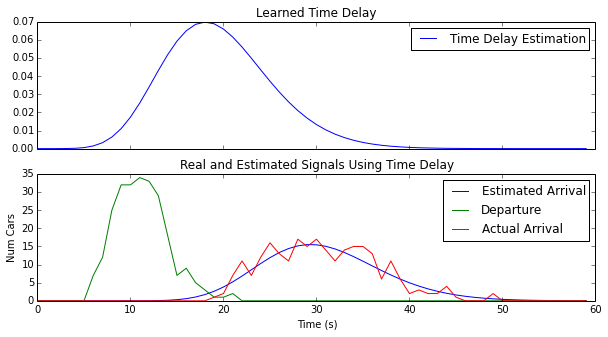
\includegraphics[scale=0.75]{figures/time-delay-est.png}
    \caption{Example time delay estimation.}
    \label{fig:time-delay-est}
  \end{centering}
\end{figure}


\subsubsection{Updating Intra-Agent Behaviour Graphs}

The second important piece in generating signal predictions is learning the intra-agent graph probabilities. 
These represent the likelihood of a signal to travel along this edge during the executed behaviours cycle.

\paragraph{Behaviour Probability Matrix (BPM)}
Figure \ref{fig:BPM-example} provides a visualization of this to help parse this idea. 
The matrix represents how these edge probabilities are used within the system; in the matrix, departing nodes are along the columns and entering along the rows -- $p_{02}$ would represent entering node 0 and exiting node 2. 
It is seen in the diagram that an event occurring at node 0 has a 60\% likelihood of exiting node 2, for this behaviour.
 It is important to not that edges that are not traversable will always have a probability of 0. 
Essentially, this probability matrix is used to split an entering signal into components, to then be combined with other estimates in a departing signal. 
This estimated signal is then used in combination with the time delay estimation to predict expected traffic, which will be discussed further in the following section.

\begin{figure}[H]
  \begin{centering}
    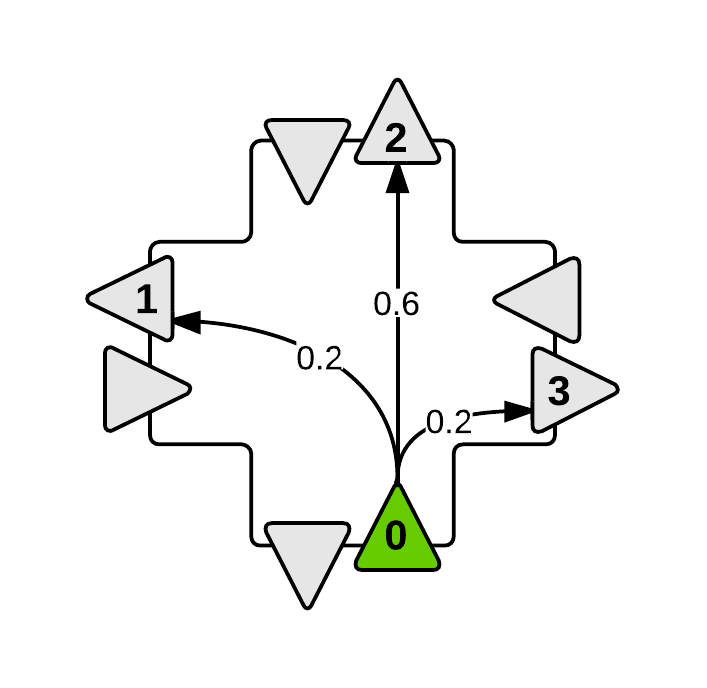
\includegraphics[scale=0.3]{figures/BPM-example.png}
    \caption{Example intra-agent edge probabilities for node 0.}
    \label{fig:BPM-example}
  \end{centering}
\end{figure}


\[
{BPM} =
    \begin{bmatrix}
    p_{00} & p_{01} & p_{02} & p_{03} \\
    p_{10} & p_{11} & p_{12} & p_{13} \\
p_{20} & p_{21} & p_{22} & p_{23} \\
p_{30} & p_{31} & p_{32} & p_{33} \\
    \end{bmatrix}
\]

\paragraph{Learning Probabilities}
This is an extremely challenging multi-objective optimization problem and multiple approaches were taken to try to solve it. 
As with the time delay estimation, this is essentially a least squares problem, but much more complex. Equation \eqref{eqn:bhvr-opt} outlines the optimization problem. 

\begin{equation*}
\label{eqn:bhvr-opt}
\begin{aligned}
& \text{minimize}
& & \sum_{j=0}^{3}\sum_{k=0}^{n} \left \| d_{kj} - \sum_{i=0}^{3}(p_{ij} c_{ki}) \ast \tau_j \right \| \\
& \text{subject to}\\
& & \sum_{i=0}^{3} P_{ij} = 1 \\
& & p_{i=j} = 0 \\
& & 0 \leq p_{i\neq j} \leq 1
\end{aligned}
\end{equation*}
Where:
\begin{conditions*}
j & outlet node \\
i & inlet node \\
k & index in sampled signal \\
d_{kj} & $k^{th}$ element in downstream neighbour arrival signal connected to agent node $j$ \\
c_{ki} & $k^{th}$ element in inlet signal at agent node $i$ \\
p_{ij} & corresponding inlet-outlet edge probability \\
\tau_{j} & time delay distribution along edge connecting agent node $j$ to neighbor \\
\end{conditions*}

This is an underdetermined system and thus cannot be solved with normal optimization methods, as is. 
The first alternative method attempted was reinforcement learning (RL).
 RL attempts to punish or reward actions for their ability to reach a desired outcome. 
In this problem, edges would be rewarded when their estimated signal closely matched a portion of the real downstream signal. 
Conversely, they would be punished when the estimated signal, over- or under-estimated the downstream one. When investigated further it was determined that this problem does not quite fit the requirements for an RL implementation and would be difficult to transform this into something that could work with existing python RL libraries (e.g. PyBrain).

Next, reducing the number of design parameters was investigated. 
For a given behaviour, some edge probabilities will always be 0 – these edges are not allowed paths – and therefore these could be removed and the problem space reduced. 
This method was determined to be infeasible due to the fact that a large set of optimization problem would need to be defined, one for each possible behaviour – the Python implementation for optimization requires that constraints be explicitly written for the procedure to work. 
Running the procedure without constraints was tested, but this failed as invalid edge probabilities were found (i.e. greater than 1 or less than 0), as expected.

Thirdly, attempting to solve the problem with a linear least squares regression model ($Ax=b$) was performed. 
The signals were taken into Fourier space to remove convolution from the equation, and parameters solved. 
The $A$ matrix in this formulation is unknown and represents the behaviour probability matrix. 
It was isolated and solved for with the formulation:

\begin{align}
	A& = DX^{T}M \\
	M& = (X^{T}X)^{+} \\
	X& = C \ast \tau
\end{align}
Where:
\begin{conditions*}
D & vector of neighbor departing signals \\
C & vector of arrival signals
\end{conditions*}

This formulation was tested and found to not produce useable results. 
Again, probabilities were found that did not fit within the required constraints.

Ultimately, the approach taken for the prototype demo was to simply have fixed BPMs for each behaviour, based on the teams understanding of traffic patterns. 
This was an unexpected technical challenge that arose as we were implementing the learning service and a sophisticated solution was not found in time. 
Discussed in later sections, we believe this problem could be fully solved with the derivation of a cost function. 
An example could be limiting the amount any edge probability can change in one cycle and penalizing ones that attempt to change by larger than this threshold – as this is likely an anomaly or incorrect identification of downstream signals.

\paragraph{Updating BPMs}
After the optimization procedure has arrived at a solution, the existing BPM must be updated. 
It would be unwise to directly use the newly calculated BPM as temporary inhibitors to traffic flow, such as accidents, can greatly skew results. 
Therefore, a learning parameter is used to update existing probabilities, seen in Equation \eqref{eqn:BPM-update}. 
This can be tuned, on an agent-by-agent basis, to alter how quickly these values are modified and adapt – an average of the two values is a good starting point, to enable quick transitions, while remaining relatively stable. 
In \eqref{eqn:BPM-update}, $i$ represents the agents ID and $BPM_{est}^{i}$ is the newly estimated behaviour probability matrix for that agent.

\begin{equation}
    BPM_{new}^{i} = \alpha^{i}  BPM_{old}^{i} + (1 - \alpha^{i}) BPM_{est}^{i}
    \label{eqn:BPM-update}
\end{equation}

\subsection{Predictions in Relay}
\label{sec:prediction_in_relay}

Making predictions of traffic is an essential component of Relay. 
This is the foundation of intelligence in the system and assists each agent in making decisions regarding behaviour execution. 
Predictions represent an estimation of local traffic $x$ seconds into the future, with the length being determined by the needs of the controller. 
Higher-order predictions, one’s that require information from the larger neighborhood, can also be generated, but with less fidelity. 
The details on how these predictions are performed is discussed below.

\subsubsection{Utilizing Neighborhood Information}
As discussed in section~\ref{subsubsec:net-top}, agents are connected to each of their neighbors, forming a grid-like mesh structure. 
This design choice allows for each agent to ``talk” with its neighbors, gaining access to all information stored. 
This ``sharing” of information is essential to keep agents informed on events occurring in the neighborhood.
Information is either requested or directly sent to a specific agent, depending on the type: current queues, predictions, plans, events, etc.
 Agents can freely communicate by simply ``asking” their neighbors for the specified data. 
An event centre is constructed on each agent to handle incoming and outgoing requests, making communication efficient and standardized across the network (discussed further in later sections).

	While an agent is not directly connected to other agents in its extended neighborhood, if required, it can indirectly access this information. 
Any agent can ``inject" requests into its neighbors to obtain information from their neighbors, and so on (again, specifics discussed in later sections). 
This isn’t used often, as fidelity decreases quickly as requests propagate outward, but, for example, it is necessary for calculating higher-order predictions.


\subsubsection{Making a Prediction}
To make a prediction, the agent must combine the learned edge probabilities with the time delay estimates for each neighboring agent. 
This utilizes previously calculated information about the agent’s in the neighborhood, to derive a predicted incoming signal for each node at the agent of interest. 
Equation \ref{eqn:first-order-pred} outlines the basic formulation for making this prediction, $Pr_{i}$, where $i$ represents the inlet node id. 
If the length of signal initially calculated is longer than the requested time, excess information will be trimmed. 
If the length requested is longer than this next-neighbor prediction, a higher-order prediction is calculated, known as $Pr_{i}^{*}$.

This information also creates useful visualizations for traffic engineers, giving them the ability to ``see into the future”. 
While they wouldn’t necessarily act upon this information, they would have an expectation of traffic at each intersection. 
It also gives context for why the next behaviour was selected (i.e. the ``plan") – this is discussed further in later sections.

\begin{equation}
	Pr_{i}^{\star} = d_{e_i} \ast \tau_{i}
	\label{eqn:first-order-pred}
\end{equation}
\begin{equation}
	d_{e_i} = \sum_{k=0}^{3} p_{kj}^{nbr} c_{k,i}^{nbr}
	\label{eqn:first-order-d}
\end{equation}
Where:
\begin{conditions*}
p_{kj}^{nbr} & edge probability for signal at $k^{th}$ neighbor node, exiting $j^{th}$ node \\
d_{e_i} & expected departing signal from neigbhor node connected to agent node $i$ \\
c_{k,i}^{nbr} & real incoming signal at $k^{th}$ node of neighbor agent connected to agent node $i$ \\
\tau_{i} & time delay distribution along edge connecting agent node $i$ to neighbor \\
k & neighbor inlet id \\
j & neighbor outlet id
\end{conditions*}


\subsubsection{Higher-Order Predictions}
As mentioned previously, if the requested prediction is longer than the neighbors can provide, a higher-order, or remote, prediction is made. 
This is performed in the same manner as a first-order prediction, but utilizes each neighbor’s current incoming prediction signal as well, $Pr_{k,i}^{nbr}$.
 If even larger predictions are required, predictions can be extended to more distant nodes, but these would be very low quality and carry low weight – these are multiplied by each intersections edge probability, intrinsically lowering their strength. 
Again, the signal is trimmed at the end to match the requested length.

\begin{equation}
	Pr_{i} = d_{e_i} \ast \tau_{i}
	\label{eqn:higher-order-pred}
\end{equation}
\begin{equation}
	d_{e_i} = \sum_{k=0}^{3} (p_{kj}^{nbr} + Pr_{k,i}^{nbr}) c_{k,i}^{nbr}
	\label{eqn:higher-order-d}
\end{equation}
Where:
\begin{conditions*}
Pr_{k,i}^{nbr} & prediction signal at $k^{th}$ neighbor node, connected to agent node $i$ \\
p_{kj}^{nbr} & edge probability for signal at $k^{th}$ neighbor node, exiting $j^{th} $node \\
d_{e_i} & expected departing signal from neigbhor node connected to agent node $i$ \\
c_{k,i}^{nbr} & real incoming signal at $k^{th}$ node of neighbor agent connected to agent node $i$ \\
\tau_{i} & time delay estimation along edge connecting agent node $i$ to neighbor \\
k & neighbor inlet id \\
j & neighbor outlet id
\end{conditions*}

\subsection{Scheduling in Relay}
\label{sec:opt:planning}

In Section~\ref{sec:def:agent} we defined the various design parameters that are necessary to implement the Relay Agent, however we omitted explicit descriptions of how particular values come to exist.
In equation~\eqref{eq:def:visible_graph} we illustrated that the Agent's transfer function (and various associated predictions/expectations) was itself a matrix-valued signal, that depended explicitly on the \emph{path} (as defined in equation~\eqref{eq:def:plan})
We then described how the behavior signal was defined in terms of the plan in equation~\eqref{eq:def:behavior_signal}.
Within this section we present the basic Relay ``Max Flow'' objective function, which is used to generate plans.
We then go on to discuss how the (somewhat naive) model could be improved with the introduction of heuristics and real-world constraints.
Ultimately, the Relay Agent should pick and execute the ``best plan'', given current predictions and biases present, taking into consideration the management of queues.

\subsubsection{The Gate Equation}
\label{sec:opt:gating}

In order to decide on the so-called `optimal' path, we must first quantify some of the primitives used extensively within this section.
The first of which is a simple linear reduction that in essence gauges the availability of a particular intersection inlet to incoming traffic flow.

\begin{equation}\label{eq:def:gating_beta}
	\beta_i(t) = \sum_{j=1}^n V_{ij}(t)
\end{equation}
In a sense, $\bf{\beta}(t)$ encapsulates the visibility or \emph{availability} of a particular \emph{gate} of the intersection.
If $\beta_i = 1$ at a particular point in time, that implies that the vehicles will instantaneously traverse the intersection, without contributing to a queue.
For convenience, we also define the complement $\phi$ in equation~\eqref{eq:def:gating_phi}, which can be interpreted as the fraction of incident traffic that is \emph{not served}, and thus will contribute to a queue.
\begin{equation}\label{eq:def:gating_phi}
	\phi_i(t) = 1 - \beta_i
\end{equation}

\subsubsection{Queue Modelling}

Within the scheduling procedure, we use relatively simple queue models, which function essentially as asymptotic Markov Queues, wherein the probability of a client being served is treated as a \emph{rate}.
Thus (at least within the prototype implementation), the notion of a \emph{queue} is more akin to an accumulator/integrator of the incidence events \emph{not served}.
The accumulator is also constantly emitting flow into the intersection governed by its availability to do so (governed by the gating signal $\beta(t)$ defined  in equation~\eqref{eq:def:gating_beta}.
In general, Relay allows accumulators that are expressed as arbitrary dynamical systems, however within the domain of queuing systems, sufficiently complex behavior can be expressed quite simply as a first-order dynamical system depending on nothing but the current state of the queue, and some input (canonically termed Markov Queues).

\begin{equation}\label{eq:def:accumulator_general}
	\frac{dq_i}{dt} = \phi_i f(t) - \beta_i g(q) u(q)
\end{equation}
where $f(t)$ is typically associated with the ingress signal (expected or otherwise), and $g(q)$ describes the rate at which accumulations are released.
This model can be expanded to arbitrary complexity, however we have found that at least in demonstrating the principle of the Relay system, simple models are more tractable (especially in simulation).
Some examples we have used succesfully are outlined in the following sub-sections.

\paragraph{Constant Relief}
With the ``Constant Relief'' model, the outflow from a particular queue is assumed to be constant, in other words $g(q) = r$, where $r$ is the rate coefficient of the queue.
The dynamics of a particular inlet's (simplified) queue are formalized in equation~\eqref{eq:def:queue_simple}.
\begin{equation}\label{eq:def:queue_simple}
	\frac{dq_i}{dt}(t) = \phi_i(t) a_i(t) - r_i \beta_i u(q(t))
\end{equation}
Which is to say that the queue length $q$ increases when incident vehicles are not being served, and decreases (releases flow into the intersection) subject to some rate parameter $r$ and the gate $\beta$ being open.

While this example serves as a good illustration (it's straightforward) it doesn't sufficiently encapsulate the dynamics of a real traffic system.
One model that does (albeit to a limited extent) is outlined below.

\paragraph{Decaying Relief}
When there are large queues, it is likely that the relief mode is congested, leading to inefficient operation (i.e.\ artificially reducing the gate).
This is encapsulated in this nonlinear queue mode depicted in equation~\eqref{eq:def:queue_exp}.
\begin{equation}\label{eq:def:queue_exp}
	\frac{dq_i}{dt}(t) = \phi_i(t) a_i(t) - r_i u(q(t)) e^{-\eta_i q(t)}
\end{equation}
Where $\eta_i$ is the associated congestion \emph{rate}, and $r_i$ as before is the uncongested rate.

\paragraph{Predictive Queue Modelling}
As alluded to throughout this section, Relay operates on a collection of time-domain signals that are defined both in the past (in terms of ingress/egress etc.) as well as the future in the form of predictions.
Since our queuing model is defined in terms of the same signals we've been using throughout, it is trivial to simulate the \emph{expected} queue state for an arbitrary time in the future.

As a tangential foreshadowing, the objective function (to be defined in Section~\ref{sec:opt:obj}) as implemented in the Prototype makes use of the separability of each inlet's queue, allowing the Agent to concurrently simulate several scenarios simultaneously.

\subsubsection{Queue-Flow Objective Function}
\ref{sec:opt:obj}
In short, Relay as a traffic control system must facilitate the efficient distribution of traffic load throughout the network.
This inevitably reduces to scheduling signal timings such that flow through the network is maximized.
While there are always additional objectives (reducing winsorized wait times, fuel consumption etc.) Relay as proposed, ultimately does not place any restrictions on the objective functions used.

Within the prototype, we chose our objective function to maximize the predicted flow through a given intersection.
In the game-theoretic sense: we take the flow-maximizing action within some finite horizon of expectation (the depth of the path).

We start by defining the sub-objective in terms of the queue differential $\frac{dq_i}{dt} = q_i^\prime$ based on the expected ingress $E[a_i](t)$, where $\Phi_i$ is the flux quantity incident on inlet $i$ over the the arbitrary forward time period $[0, t]$.
\begin{align}\label{eq:def:sub_objective1}
	\Phi_i &= - \int_0^t q^\prime_i(\tau) d\tau\\
	&= \int_0^t \beta_i g_i(q_i(\tau)) u(q_i(\tau)) - \phi_i E\left[a_i\right](\tau) d\tau
\end{align}

By substituting equations~\eqref{eq:def:gating_beta},\eqref{eq:def:gating_phi}:
\begin{equation}\label{eq:def:sub_objective2}
	\Phi_i(\beta_i) = \int_0^t \beta_i \left(g_i(q_i(\tau)) + E[a_i](\tau)\right) - E[a_i](\tau) d\tau
\end{equation}
Noting that $\beta_i$ is defined in terms of the agent's visible graph as of equation~\eqref{eq:def:gating_beta}, which is in turn defined based on the behavior signal.
Thus all other factors remaining constant, the inlet flux $\Phi_i$ is the result of an explicit function of the behavior chosen, and thus the underlying path.

Ultimately, the total biased-flow through the intersection, as a function of the plan $p$ which parametrizes $B$ by~\eqref{eq:def:behavior_signal}, which in turn defines $\beta$ via equation~\eqref{eq:def:gating_beta}.
\begin{equation}\label{eq:def:biased_flow}
	\bf{\Phi}_p = \sum_{i=1}^n \Phi_i
\end{equation}

The objective is as follows: Choose the plan $p$ such that the aggregate inlet flux $\bf{\Phi}_p$ is maximized.
Subject to the constraints implied in the definition of $p$ (equation~\eqref{eq:def:plan}).
\begin{equation}\label{eq:def:combined_objective}
	\argmax_p \bf{\Phi}_p
\end{equation}
Subject to:
\begin{align}
	d &\leq d_{max}\\
	t_d &\leq t_{max}
\end{align}
recalling that $d$ is the depth of the path $p$, and that $t_d$ is the last time associated with the path.
Further recall that all constraints placed on the validity of a particular path are encapsulated in the definition of the path $p$, (i.e. they must be temporally successive, and infinitesimally short steps are prohibited via the Behavior Transition Graph).

Note this is a combination set-cover (NP-complete), and nonlinear programming problem.
For efficiency, it is best to separate the integer aspect out (separate out the time component of the path from the graph component).
This is described below:
\begin{equation}\label{eq:def:minlp_objective}
	\argmax_{p.B} \argmax_{p.t} \bf{\Phi}_{p.B}
\end{equation}
where $p.B$ is the sequence of behaviors (irrespective of their relative timing), and $p.t$ is the timing (given a behavior sequence $p.B$.
Thus for each behavior, we evaluate the best possible flux given changes to the relative timing, and use the combination $p =  (p.B, p.t)$ that gives the best outcome.

\subsection{Agent Implementation}

The Relay Prototype implementation was designed according to our functional requirements.
Agents must be able to communicate their state to a third party (i.e. the Back-End), and pass messages to their immediate neighbours (as defined in a connectivity graph used to initialize the network).
The Agents must 

\subsubsection{Actor Pattern}
Each agent was designed as a concurrent Erlang \emph{application}, consisting of several concurrent, asynchronous actors.
Erlang was chosen for this purpose as it is a language with a history of soft-realtime computing in telephony (via the Open Telecom Platform), as well as exposing an easy and intuitive message passing interface (in that the only way for actors to communicate is via message passing).

In this manner it was possible to communicate ``over the wire'' to a myriad of simulated Agents all operating concurrently in simulation within a single Erlang Virtual Machine (VM), and furthermore, this communication was relatively straightforward, and didn't involve writing HTTP/TCP adapters.
Additionally, through the use of OTP-\emph{applications}, there is pragmatically no difference between multiple Agents being simulated on a single machine communicating with each other, and multiple agents being simulated on different, geographically separated machines, communicating with each other (albeit with the obvious increase of latency).

\subsubsection{Number Crunching}
If concurrent operation, scalabilty and fault-tolerance are Erlang's strengths, floating point work (colloquially ``Number Crunching'') is one of its most predominant weakness (in the context of implementing Relay).

We used ErlPort, a Library that utilizes Erlang's Port-protocol to interface natively between operating system processes running the Erlang VM, and Python respectively.
Thus whenever a particularly numerical computation needed to be performed (i.e. generating predictions, batch reinforcement learning, and scheduling), the associated Agent (whose existence is encapsualted within a particular Erlang application), would submit a request to the Python port, which would perform the computation, and return the result asynchronously.

Python with (NumPy) was chosen to facilitate the optimization and machine learning (massive floating point work) algorithms associated with an individual agent.
An additional advantage (from the prototype implementation/simulation perspective) was that a single Python ``workhorse'' process could be shared by more than one Relay Agent, thus preserving OS resources on the host machine running the simulation, and allowing us to simulate additional Agents concurrently.


\newpage
\chapter{Design Testing and Validation}

\section{Front End}
\subsection{Use Case Analysis}
As part of the iterative design process employed during this project, a Use Case Analysis was done by members of the team, as well as at the Design Symposium, utilizing feedback on the demo application from members of the public to help validate the success of the implementation, in the context of the previously established Use Cases.
Users of the demo were taken through each of the implemented Use Cases, and their level of fulfillment was determined.
It should be noted that the Roads functionality was not included in the demo, thus Use Cases 3, 5, and 8 are not included in the Use Case Analysis.

\noindent \textbf{UC1: User monitors network map} \\
This Use Case was found to be successful with all users.
As this is the default page of the application, which is first presented on page load, all users were able to successfully monitor the map for activity and high-level network performance.

\noindent \textbf{UC2: User monitors intersection list} \\
This use case was also successfully implemented through the demo, and many users were able to accomplish this task without error.
The clear global navigation in the header of the application, as well as the simple page design for the Intersections page made navigating to and monitoring the list of intersections for activity easy.

\noindent \textbf{UC4: User searches for an intersection} \\
Through the use of  recognizable UI elements for the search/filter design on the intersections page, this feature was easily found and used by most users.
A small bug in this feature was recognized at this stage, wherein the filter does not update as the user makes an edit to the search query. 
As a result, a refresh of the page was required to continue searching for intersections, which generated relatively negative responses from the users.

\noindent \textbf{UC6: User inspects network details} \\
While this action is somewhat hidden in the application, along the side of the screen, most users were able to navigate to the details dashboard without issue, as multiple paths to reach it were designed into the interaction of the application.
Common, recognizable icons were used to open this dashboard, which provides visual affordance for users, making the access of this dashboard intuitive.
This played a large part in reducing confusion and errors with users looking to access this screen.

\noindent \textbf{UC7: User inspects intersection details} \\
This interaction was found to be very natural for users.
With data layers positioned on the map, it was found that most users had a natural tendency to pan, zoom, and click on data points that are located on the map, with the intention of seeing more information.
This intention comes from most users' experience with other mapping software that behaves in a similar fashion.
Clicking on a data point on the map activates the info box window, which contains information on signal status, phase, performance level, bias vector, and flow characteristics.
This made accessing any of the required data simple, and easy for many users.

As a result of this Use Case Analysis, it was found that users reacted to each task with a high level of ease and satisfaction.
Next steps include continuing to build out the Roads functionality, such that the remaining use cases can be satisfied, as well as mending the bug found with the search/filter functionality on the Intersections page.

\subsection{Functional Requirements Analysis}

The initial functional requirements which drove the development of the solution will be used to test the application. Requirements are divided into three sections: Network Requirements N1 -- N4, Intersection Requirements, I1 -- I9, and Road Requirements R1 -- R7. The functional requirements assessment is outline in table \ref{table:freqassessment}. Each functional requirement will be assesed for whether the requirement has been implemented within the interface. In order to test this, the design team reviewed the final implementation of the Relay Front End application by deciding whether the functional requirement in question was true. For example, given requirement N1, the design team decided that it was indeed possible to see all of the intersections in the network on a map, thus the functional requirement was marked as completed.

\begin{longtable}[H]{| P{6.5cm} | P{2.5cm} | P{6cm} |}
    \hline
    \textbf{Requirement}                                                                            & \textbf{Status}        & \textbf{Comments}                                                                              \\ \hline
    N1: See all of the intersections in the network on a map.                              & Completed     & ~                                                                                     \\ \hline
    N2: See a list of all of the intersections in the network.                             & Completed     & ~                                                                                     \\ \hline
    N3: See the performance metrics of the network.                                        & Not Completed & Functionality was developed in the application but network statistics were not shown. \\ \hline
    N4: See the history of the performance metrics for the network.                        & Not Completed & See N3.                                                                               \\ \hline
    I1: See the status of all of the intersections in the network.                         & Completed     & Intersection information is currently only available through the map interface.       \\ \hline
    I2: See basic performance information about all of the intersections in the network.   & Completed     & See I1.                                                                               \\ \hline
    I3: Search for an intersection in the network and see the details of the intersection. & Completed     & See I1.                                                                               \\ \hline
    I4: See an intersection's position on a map.                                           & Completed     & See I1.                                                                               \\ \hline
    I5: See basic information about the intersection.                                      & Completed     & See I1.                                                                               \\ \hline
    I6: See the status of the intersection.                                                & Completed     & See I1.                                                                               \\ \hline
    I7: See the signal state of the intersection.                                          & Completed     & See I1.                                                                               \\ \hline
    I8: See current performance metrics of the intersection.                               & Completed     & See I1.                                                                               \\ \hline
    I9: See the history of the intersection's performance.                                 & Completed     & See I1.                                                                               \\ \hline
    R1: See the status of all of the roads in the network.                                 & Not Completed & ~                                                                                     \\ \hline
    R2: See basic performance information about all of the roads in the network.           & Not Completed & ~                                                                                     \\ \hline
    R3: Search for a road in the network and see the details of the road.                  & Not Completed & ~                                                                                     \\ \hline
    R4: See the road on a map.                                                             & Not Completed & ~                                                                                     \\ \hline
    R5: See basic information about the road.                                              & Not Completed & ~                                                                                     \\ \hline
    R6: See the current performance of the road.                                           & Not Completed & ~                                                                                     \\ \hline
    R7: See the history of the intersection's performance.                                 & Not Completed & ~                                                                                     \\ \hline
\caption{Solution Assessment for Functional Requirements.}
\label{table:freqassessment}
\end{longtable}

Only 50\% of network-level functionality was met in the final application prototype. N1 and N2 relate specifically to the display and understanding of intersection performance, which is a core aspect of the application. N3 and N4 relate to network-level metrics. The Front End application was built to support network information, and a network-specific page was developed to display metrics, time-series graphs, and activity lists. These metrics were not available in any meaningful manner from the Back End. Although all necessary information for performing such calculations was available to the Front End, it was not appropriate to require the Front End to perform this task. Therefore, the information was not made available in the interface for the final solution.

All of the intersection functional requirements --- I1 through I9 --- were met in the final solution. However, this functionality was only available through the map view in the interface. An intersection-specific, list-based interface was developed, however the intersection-specific functionality requirements I1 -- I9 were not supported. Therefore, the functional requirements have been technically met, yet they are not ideal.

None of the Road-based functional requirements were completed. During the implementation of the solution, it was realized that rich information along road edges would not be available. The final Front End solution does have interface components for supporting road information. This was done as a proof-of-concept for the value of having road information accessible. However, no real data was available.

Overall, the Front End solution met a sufficient amount of functional requirements to demonstrate the value of the solution. However, important functionality is either missing or for demonstration purposes only. Therefore, significant work must be done to reach a suitable level of quality for implementation.

\section{Back End}

As the intermediate layer between the Relay Framework, and the Relay Interface, the back-end performs little in the way of computation (other than ETL associated with communication).
Thus the main requirement is to respond to requests from the Relay Interface promptly.
Noticeable lag between modules, especially as it relates to the interface can dramatically reduce the end-user experience.
While this may not be of paramount importance for prototyping, it does become useful during development, and is further exacerbated by our technological constraints (hosting the platform locally on our personal computers).

That said, within the realm of software development there are a large battery of tests/testing-related-philosophies that could see application within this project.
At the highest level, system integration tests will be used to ensure platform robustness, especially in development.
At the code module level, the typical suite of unit tests will be used to assert correctness.
However, due to time requirements, rigorous testing is neither wanted nor warranted, and as such only the most critical systems will be tested in this way.
For example, the request handler is invoked every time the Interface needs new information, this module should be exceptionally robust to failure.
In a similar fashion, database connections can involve a significant amount of complexity if handled poorly.
Within this respect we follow the motto that the architecture should guide development to reduce the likelihood of system failure.
In this string, we have endeavored to architect the Relay system as multiple pseudo-independent modules, each with their own functional (correct) core.
This design pattern is commonly referred to as ``Ports and Adapters'' or ``Hexagonal Architecture''.

\subsection{Integration Testing}
The following integration tests are all pass/fail procedures aimed to ensure each module is functioning. 
These tests will demonstrate that disparate pieces of the system work together. 
These tests are centered on the Flask server, and cover information and request handling from the Interface, Framework, and database. 
The table below contains each test and results from testing on the final prototype.

\subsubsection{Results}
As seen in the above table all integration tests have passed. All subsystems within the application can successfully communicate with one another. Each module can interpret the requested information and perform the desired actions.

\begin{longtable}[H] {| P{3.5cm} | P{10cm} | P{1.5cm} |}
    \hline
    Test                             & Description                                                                                                 & Results \\ \hline
    Handle requests from Interface   &  Interface can pass POST and GET requests to Flask server for processing.                                   & Pass    \\ \hline
    Return data to Interface         &  Server successfully returns requested information to Interface. Data is parsable and useable by Interface. & Pass    \\ \hline
    Make Requests to Framework       &  Server can make HTML requests to Framework through Python requests library.                                & Pass    \\ \hline
    Handle data sent from Framework  &  Server successfully handles and parses requested.                                                          & Pass    \\ \hline
    Make requests to SQLite database &  Server can query associated database through Python sqlite3 library.                                       & Pass    \\ \hline
    Handle data sent from database   &  Server successfully handles and parses requested information from database.                                &  Pass   \\ \hline
\caption{Integration tests for Flask Server}
\end{longtable}

\section{Deep End - Relay Framework}
\subsection{Integration Testing}
The following integration tests are all pass/fail procedures aimed to ensure each module within the Relay Framework is functioning. 
These tests will demonstrate that disparate pieces of this system work together. 
These tests are centered on the components of the Framework, and cover information and request handling from the Flask server, between Erlang processes, Python computational components, and <OTHER>. 
The table below contains each test and results from testing on the final prototype.

\subsubsection{Results}
As seen in the above table all integration tests have passed. All subsystems within the Framework can successfully communicate with one another. Each module can interpret the requested information and perform the desired actions.

\begin{longtable}[H] {| P{3.5cm} | P{10cm} | P{1.5cm} |}
\hline
    Test & Description & Results \\ \hline
    Request data from neighbouring agents                                                                            & The agent of interest (Erlang process) can request information from the other agents (processes) connected to it. & Pass    \\ \hline
    Handle data from neighbouring agents                                                                             & After requesting, the agent can successfully accept and interpret information.                                     & Pass    \\ \hline
    Accept requests from neighbouring agents                                                                         & Can successfully accept requests and return information to neighbouring.                                          & Pass    \\ \hline
    Request prediction from Python prediction service                                                                & Can request a new prediction from Python prediction service.                                                      & Pass    \\ \hline
    Handle data from prediction service                                                                              & After requesting a new prediction, can successfully accept and interpret information.                              & Pass    \\ \hline
    Request updated time delay estimation and/or behaviour probability matrix from Python parameter learning service & Can request a new time delay and behaviour probability matrix from Python prediction service.                     & Pass    \\ \hline
    Handle data from parameter learning service                                                                      & After requesting new parameters, can successfully accept and interpret information.                              & Pass    \\ \hline
\caption{Integration tests for Relay Framework}
\end{longtable}

\newpage
\chapter{Recommended Design Modifications}

\section{Front End - Relay Interface}
Upon building the Relay Interface to a stage where it was usable, testable, and demo-able on Symposium day, a number of areas were identified where future design and development efforts should be placed, in order to improve the overall usability and experience of the application.
These areas for future development include both the front-end User Interface design, as well as the Application Architecture itself to help create a more robust product both internally and externally.

\subsection{User Interface}
Given more time and design/development efforts, there are a number of areas in the User Interface of the Relay application that could be modified to better serve the needs of consumers and Traffic Engineers.
The first area would be to improve the execution of searchable list views within the application.
These currently reside on the Intersections and Roads screens.
Design recommendations for list views would be to build out further interaction with the lists, to provide as much insight into the data as would be found by inspecting an intersection from the map screen.
This could be done by creating a side panel on the Intersections and Roads pages that would be activated by clicking a row on the table.
Given that the tables currently require no more than two thirds of the screen width to be displayed, a side panel with in-depth data would fit well on the screen, perhaps filling the remaining one-third of the page.
Furthermore, a small bug was found with the search/filter functionality that makes using that feature a bit cumbersome.
When a list is filtered, and the search query is removed or edited to perform and new search, the table does not currently update and the page must be refreshed.
By implementing the list filter as a fully dynamic feature, where search edits can be made continuously, the experience of using lists to locate roads and intersections in the Relay application will be greatly improved.

A second recommended design modification is to continue building out the Network page.
While the power of the average laptop is able to power and simulate approximately 10 live Relay-controlled intersections, more power is necessary to truly understand the data from a large network, such that would be suitable to display on the Network page.
As a result, live full-network metrics were difficult to provide, thus it is recommended that the Network page and corresponding data be tested further on a more powerful system, to truly see the effectiveness of the data being visualized.
Metrics to explore here include charts displaying overall network delay/queue length, and network flow.
Full-network metrics were identified as important in the User Study, and so it would be critical to continue to optimize the Network page for future implementations.

Further recommended design modifications for the User Interface of the Relay application include building out the Roads page and functionality.
Desired features involving road data were unable to be built to a usable high-fidelity state, and so focus should be placed on this area for future implementations.
The Roads page, when built, should look and behave similarly to the Intersections page, such that the same learned skills and interactions from the Intersections page can be applied directly to the Roads page.
They should not be so similar, however, that they become confused for one another, so it should be ensured that there are enough distinguishing factors for each, so as to reduce confusion for the users.
This would include providing an improved list-view for all of the roads in the network, as well as corresponding metrics and attributes to help identify roads that require the attention of a traffic engineer.

Expanding this road functionality should include the ability to highlight arbitrary roads on the map.
This functionality could be embodied in a number of features, such as highlighting the roads connecting intersections that are currently communicating with one another, perhaps when a particular intersection is clicked by the user.
This would provide even further insight, particularly to Traffic Engineers, into the way the system is behaving and the decisions it is making.
Engineers should have as much understanding of the system as possible, and so a feature such as this would help to improve such an understanding.
Road highlighting also has other interesting applications for consumers, particularly in the area of route planning.
With the ability to place graphics along a roadway comes the ability to highlight any arbitrary route through the network.
This opens up a large feature-space in the Relay application to promote consumer usage, as many people using mapping applications for their routing abilities.
As road highlighting presents numerous positive feature implementations - for both consumers and traffic engineers - its design and development should be pursued further, given additional design and development time.

Finally, recommended design modifications come in the area of data visualization layers.
Given the vast amount of ways one can portray a given data set, it is recommended that this area of the application be continually modified and improved over time.
Different metrics should be explored in this area, outside of the current Status, Flow, and Queue Length implementation.
More metrics that are important to traffic engineers, in different visualization forms, will be beneficial in providing a useful application to the widest possible base of users.
Other ways to graphically show detailed, quantitative information on the map should also be explored here, possibly in the form of overlays or modular windows atop the base map.
Building on the idea of a ``quick look'' into an intersection, as shown in the info box implementation, would be beneficial in providing the best possible browsing experience that suits the workflow of traffic engineers.
Continued design in development in any or all of these recommended areas is expected to improve the overall quality of the Relay User Interface, thus better satisfying the needs of target users.
With ever-changing and often unpredictable data, diligence must be paid to the continued refining of visualization techniques and best practices in the interface.
Other considerations and recommendations can be described through changes to the application architecture, as explained in the next section.

\subsection{Application Architecture}

Ideally, the Relay application would be available to both public workers responsible for the network and the public at large. These two groups have fundamentally different needs and requirements, and thus should see different application interfaces. For example, a citizen may want to see only delay times on roads, whereas a traffic engineer may want more detailed metrics, such as mean delay time, flow volumes, and queue lengths. Furthermore, individuals accessing the application will have differing levels of responsibility and privilege. For example, a citizen might be able to view the direction bias at intersections, whereas a traffic engineer may be able to edit the direction bias to account for discrepancies in the model.

These differing user requirements motivate the need to implement user-based authentication for access into the system. The application should be enhanced so that users are required to log in in order to access the application. The Relay application can then customize the application to the specific needs of the user. Furthermore, user-specific authentication will allow for more detailed collection of usage data. This usage data can help the transportation authority better understand the involvement of various members.

As the application may have the potential to modify settings within the Relay network, therefore modifications must be made to ensure application security. As discussed above, the introduction of login-based authentication will limit access to sensitive functionality. The use of data encryption on information transmitted between the client and the server should also be explored. Depending on the inputs to the Relay network, inputs should require validation and be cleaned to remove all malicious inputs.

The Google Maps API provided sufficient functionality for the scope of this project. However, there were various drawbacks which would be unacceptable for a production-level implementation of the Relay System. An ideal mapping library would have no usage limits, which would prevent unexpected disruption of service to users. It would also allow for complete customization of map styling to ensure the visualizations can be presented in an optimal and professional manner. Finally, an ideal mapping library would allow for the implementation of fully-customizable features, such as markers and info boxes. This prevent unnecessary complexity and performance issues as a result of working with sub-optimal native features.

Usage of the demonstration prototype highlighted the performance issues associated with large amounts of network information. Specifically, some visualizations performed noticeably slower on large quantities of information. As such performance issues are unacceptable in production-level applications, it is suggested that further work be done to improve the performance of such applications. The use of Google Maps API native functionality for presenting visualizations as likely the cause. In the future, custom visualization functionality should be built to optimize for performance with large volumes of information.

\section{Back End}

\subsection{Client-Server Communication Improvements}

The existing implemented API was sufficient for demo purposes. However, it is limited in it's functionality, modularity, and scalability. The current API architecture is designed specifically for the information requirements defined in the solution. This means that any future solutions would require new API calls to be added to the architecture. Furthermore, the existing API architecture does not have the full range of functionality required for a production-level application.

First, the API should be converted to a Representational State Transfer (RESTful) API architecture. RESTFul allows for the hierarchical representation and access of information from the server. Following this method greatly increase the modularity of the API, making it more accommodating to future changes in the application, and preparing the system for potential public use.

Second, the API should provide richer functionality for specifying request details. Enhancing API requests to consider parameters such as maximum count and other filtering parameters improves performance by preventing the transfer of unnecessary data from the server to the client.

Switching to a RESTful architecture and implementing richer parameter support both improve the scalability and robustness of the API, which are crucial features for such a critical application.

WebSocket technology takes a fundamentally different approach to client-server communication. Instead of making multiple synchronous HTTP requests to a server over time, WebSocket technology establishes a single connection between the client and server, or which information is streamed as necessary. This greatly improves performance and scalability, as large HTTP requests can be send bit-by-bit in a constant stream. Furthermore, it allows for real-time updating for information, which is not bound to the updating schedule of the client. Unfortunately, WebSocket technology is relatively new and immature in comparison to HTTP communication, and thus does not have the necessary reliability and support to be the sole communication technology in this situation.

WebSocket technology should be implemented in the Relay Application as an enhancement to the existing HTTP channels. If available, the WebSocket could be used to improve performance by sending localized, real-time updates of traffic data to the client, while lowering the update frequency of HTTP requests. HTTP requests could then be used for initialization purposes, such as gathering static data and initial data loads.

\section{Deep End - Relay Framework}
\subsection{Integrating Auxiliary Information}
In the future, we would give our adaptive traffic system the ability to be modified for region and time specific parameters. 
This would entail modifications for specific road conditions, neighbourhoods, and/or weather.
Adapting for changing weather and road conditions improves the safety of travellers through the system by changing signal timings to reflect changing driving speeds.
For example, in icy conditions rather than improve intersection volume, it could hypothetically be more beneficial to reduce the amount of acceleration undergone by vehicles, resulting in a lower average speed, but safer transportation environment for all.
By optimizing for these new conditions it would attempt to ensure traffic is still flowing smoothly.
Incorporating more external data, such as school times, locations, and days, would allow the system to dynamically control car flow through school zones.
This would help to increase safety in these areas by working to either route cars away from these zones, or adapting to reflect slower speed limits during ``school hours''.
These types of biases would then be tested in simulations, and performance improvements measured.

\subsection{Utilize Historical Data}
This is related to the previous point of ``Integrating Auxiliary Information”, but would come from within the system. The system was not run long enough to collect ``historical” data, but it is recommended that future development work incorporate this information in the optimization procedures. 
By utilizing historical trends, the system can better predict expected traffic flows and ultimately perform better. 
Additional request handlers could be attached to optimization processes to accept this information and incorporate it into the calculations. 
For example, if it is notified of an upcoming sporting event, it could look back at previous events and their impact on traffic flows. 
This information could then be used to bias signal plans to accommodate the expected traffic.

Historical trends and data could also be exposed through the Flask server to the Interface. 
This could provide useful insights for traffic engineers and the general public, identifying times of high traffic and assisting in route planning.

\subsection{Exploiting Neighborhood Redundancy - The ``Super Node"}  % Possibly redundant.
Future research could be conducted to tackle the challenge of optimizing network communication within the purview of the neighbourhood mesh network topology.
This was not a primary concern of this project, but it is mentioned here for completeness and as a possible stepping stone for further research.

As was mentioned in the discussion on network topology and Framework architecture, multiple agents will have very similar information about each other.
It is possible to exploit this redundancy to efficiently store copies of network-wide data either for posterity or to introduce more convenient mechanisms to access the information.
An example of such a use-case is the Data Processing module within the Relay Back-end system.

Similar to raft-consensus models, we could introduce a distributed ``Super Node'' selection policy within the network.
Such a policy entails the Agent network to elect (from their own ranks) a \emph{Super Node} to act as a data uplink to external services for particular pieces of data.
For example, in the case of a neighbourhood of Agents, the region can elect a member (perhaps based on hardware capability, stability, trust, or other metrics out of the scope of this project) to act as the external point of contact or liaison for external services wishing to access the network data.
Similarly, these Super Nodes would be allowed to break the \emph{network depth} requirement enforced by our network topology, and communicate/subscribe to other Super Nodes.
Network updates could be pushed externally to a single Super Node, which would be responsible for gossiping the update to its peers, and neighbourhood.

\subsection{Robust Simulation Environment}
In the future, the team proposes integrating a robust simulation environment to assist in extracting in depth performance metrics and modelling complex road structures. 
PTV Vissim is a commercially available product, provided by the University, but the team did not have adequate resources to integrate it into the system. 
As identified in earlier reports, it is difficult to programmatically interface with the application and significant time is potentially required to set up a complex environment. 
The team would either attempt to build an environment using Vissim, research other solutions, or continue building out our own custom simulation tools.

\subsection{Updating Behaviour Edge Probabilities}
As discussed in the engineering approach for ``Learning in Relay” a sophisticated solution for behaviour edge probability learning was not found.
 Further research and development would need to be conducted to derive a solution to his problem – the system is underdetermined, and either requires a reduction of design parameters or other reformulation to become solvable. 
A method that we propose is to use a cost function to constrain some aspect this problem. 
An example could be penalizing probabilities that change too drastically and limiting them within some threshold. 
A target could also be set on total error in the system with penalty terms added. 
This is just an example of an approach that could be taken, and development and testing would need to be performed.

\subsection{Exposing Higher Detail Performance Statistics}
With the implementation of a robust simulation environment, more performance statistics would become available. 
Infrastructure could then be built on the back-end to store and expose this information to the Interface.
Increasing insight into the system would provide traffic engineers with greater understanding of the performance of the current models and network as a whole.

\newpage
\chapter{Timeline and Project Management}

\section{Tasks and Deliverables}

\subsection{Fall 2013}
Below is an overview of the tasks to be completed over the Fall 2013 term. 
These outline the major milestones and steps that will be taken to create the first prototype, presented at the end of this term. 
The description column goes into detail about what will be performed in this task, and in many cases describes what will be included in that tasks deliverable. 
The deliverable column, where applicable, identifies the high-level product of each specific task.
\\

\begin{longtable}[htbp] {| P{2.5cm} | P{10cm} | P{2.5cm} |}
    \hline
    Task                                       & Description                                                                                                                                                                                                                                                                                                                                                                                & Deliverable                                        \\ \hline
    Idea Generation (W0-W1)                    & Researched existing solutions that attempt to tackle the problem or interest, or something similar. Brainstormed ideas and identified shortcomings of existing products to determine specifications and features of our proposed solution. Researched applicable technologies that will be potentially useful in building solution. Met with supervisor to gain initial thoughts. & N/A                                                \\ \hline
    Design Proposal (Oct 11)                   & Outlining and detailing the proposed design project idea. State of the art, needs analysis, and design specifications and requirements are provided.                                                                                                                                                                                                                                       & Report                                             \\ \hline
    Gain Supervisor Insight (W2)               & Meet again with supervisor to discuss our proposed idea and plan. Get his insight on our solution/plan/etc. and input on what we could change or improve.                                                                                                                                                                                                                                  & Copy of Design Proposal                            \\ \hline
    Design Proposal Presentation (W2)          & Presentation of project proposal. Summarize contents of report and gain feedback from classmates on idea. This will be a project `defence' and will also gain feedback from MBET students.                                                                                                                                                                                                 & Presentation and slides                            \\ \hline
    Design Critique/ Feedback (W2)             & Submit an assessment for two other projects both during presentation and prototype demo.                                                                                                                                                                                                                                                                                                   & Report                                             \\ \hline
    Low-fidelity Simulation Design (W3)        & Based on proposal, begin designing simulation environment for underlying system. This will be a set of wireframes and sketches of the final product. The team will discuss and iterate on these until a final design is chosen.                                                                                                                                                             & Wireframes and sketches of proposed solution       \\ \hline
    Early System Architecture (W3)             & Based on proposal begin designing and further researching each of the initial ideas. Obtain better understanding of what will be required to be developed (e.g. intersection network). Decide what technology will be used (e.g. CartoDB).                                                                                                                                                 & System architecture design and required technology \\ \hline
    Ongoing Research and Learning (W3 - W5)    & Perform further research on technologies and knowledge required to construct system. Will need to learn concepts in: machine learning, neural networks, network programming, distributed systems, and simulating these types of systems.                                                                                                                                                   & N/A                                                \\ \hline
    Update Meeting (W3/4)                      & Meet with supervisor to discuss current progress. Bring up any difficulties we are having and work through these.                                                                                                                                                                                                                                                                          & N/A                                                \\ \hline
    Mid-Fidelity Design (W3 - W4)              & Basic Quartz Composer mock-up created. This will have interactions developed and will allow us to iterate and improve the simulation environment.                                                                                                                                                                                                                                          & Quartz Composer mock-up                            \\ \hline
    Mid-Fidelity System Architecture (W4 - W6) & Designing functionality of ``actors'' (i.e. intersections). Begin development of network architecture (how do you connect all actors together?). Further research of programming paradigms required to construct the system.                                                                                                                                                                 & Architecture designs                               \\ \hline
    High-Fidelity Simulation Design (W6)       & High quality quartz composer mock-up. Have all basic functionality designed and prototyped. UI assets designed/created.                                                                                                                                                                                                                                                                    & Quartz-Composer mock-up                            \\ \hline
    Initial System Development (W6 - W7)       & Begin construction of system: ``agents'', ``network'' components, application infrastructure. Begin designing/building interfaces with sim-env.                                                                                                                                                                                                                                                & N/A                                                \\ \hline
    Sim-env Dev (W7-W8)                        & Begin developing the simulation environment. Create basic features.                                                                                                                                                                                                                                                                                                                        & Passes unit tests                                  \\ \hline
    Finish Prototype System Dev (W7-W8)        & Ability to set-up a network of actors, actor functionality established, and actors able to `talk' to each other.                                                                                                                                                                                                                                                                           & Passes unit tests                                  \\ \hline
    Simulation and System Testing (W8-W9)      & Testing of sim-env and system for prototype demo. Fix any issues that arise.                                                                                                                                                                                                                                                                                                               & Passes unit tests                                  \\ \hline
    Design Critique (TBD)                      & This will be a presentation to a group of ``Dragon's''. Similar to design proposal presentation and group will defend the proposed idea and solution. Will go in depth in how the solution is superior to current state of art.                                                                                                                                                              & Presentation and slides                            \\ \hline
    Prototype Demo (Nov 29)                    & First demo of project. Team will present the first prototype that has been created. Will identify challenges that arose, what modifications needed to be made, and what the next steps will be to reach end goal.                                                                                                                                                                          & Presentation, demo, and slides                     \\ \hline
    Design Brief (Dec 7)                       & ~        Summary of progress this term.                                                                                                                                                                                                                                                                                                                                                                                   & ~           Report                                       \\ \hline
    Outreach Presentation (TBD)                & Participate in UW sponsored event to demonstrate project. Will be used to showcase SYDE design projects and gain outside feedback on our project.                                                                                                                                                                                                                                          & ~                     Presentation, summary.                             \\ \hline

\end{longtable}

\subsection{Winter 2014}
Below is an overview of the tasks to be completed over the Winter 2014 term.
These outline the major milestones and steps that will be taken to create the final prototype, presented at the final symposium.
The description column goes into detail about what will be performed in this task, and in many cases describes what will be included in that tasks deliverable.
The deliverable column, where applicable, identifies the high-level product of each specific task.\\

\begin{longtable}{|p{4.5cm}|p{6cm}|p{4.5cm}|} \hline
    Task                                              & Description                                                                                                & Deliverable                           \\ \hline
    Team Debrief, Update (W1)                         & After the Holiday's team will meet over the first few weeks to get back up to speed with what was accomplished the previous term and over the break as well. Will begin creating a detailed list of tasks to be completed.         & N/A                                   \\ \hline
    Response to Feedback (Jan 21)                     & Details of this report TBD                                                                                                                                                                                                         & Report                                \\ \hline
    Meet with Supervisor (W2)                         & Meet again with supervisor to discuss our progress and plan. Get his insight on our solution/plan/etc. and input on what we could change or improve.                                                                               & N/A                                   \\ \hline
    Actor Development and Research (W2)               & Continue building functionality of ``actors'' (i.e. intersections). Begin development of network architecture (how do you connect all actors together?). Further research of programming paradigms required to construct the system. & Architecture designs and construction \\ \hline
    Application Development (W2)                      & Continue iterating on current interface/interaction design. Add more features (e.g. advanced traffic information panel) and incorporate newest functionality from back-end.                                                        & Updated interfaces and application    \\ \hline
    Network Development (W3-W4)                       & Ability to set-up a network of actors, actor functionality established, and actors able to ?talk? to each other.                                                                                                                   & Passes unit tests                     \\ \hline
    Online Predictive Model Prototyping (W4-W5)       & Begin prototyping algorithms for controlling the network. Will utilize knowledge gained from researching other systems and reading papers on current state of the art.                                                             & Direction to proceed with algorithms  \\ \hline
    Small Network Trials (W4 - W5)                    & With algorithms, perform tests with a small network of actors (e.g. 2-5 nodes). Iterate on designs as needed. Also, connect with front-end to test data streaming capabilities.                                                    & Passes network tests and benchmarks   \\ \hline
    Update Meeting and Simulation Research (W4/5)     & Meet with supervisor to discuss current progress. Bring up any difficulties we are having and work through these. Continue investigating simulation environments. May revise timeline after decision about this is made.           & Simulation environment understanding  \\ \hline
    Prototype Update Demo/ Feedback (Jan 31 - Feb 11) & Present updated prototype. Show current progress and gain feedback from peers. Make changes to solution based on this where needed.                                                                                                & Feedback, Presentation                \\ \hline
    Online Predictive Model Development (W5 - W6)     & Based off prototype and testing conducted, formalize the algorithms to be used in traffic control. May updated after large-scale network tests completed                                                                           & Passes network tests and benchmarks   \\ \hline
    Application Development (W6)                      & Continue adding features to the interactive application. Integrate more features with back-end                                                                                                                                     & Refined application experience        \\ \hline
    Larger Network Tests (W6 - W7)                    & With algorithms, perform tests with a larger network of actors (e.g. \~50-100 nodes). Changes to model will be made based on the results of this.                                                                                  & Passes network tests and benchmarks   \\ \hline
    High-Fidelity Model Development (W7-W8)           & Continue adding features to algorithms, improving stability, testing network, and providing information for front-end                                                                                                              & Passes unit tests                     \\ \hline
    High-Fidelity Application Development (W7-W8)     & Finish developing application. Test all functionality to ensure it meets the goals.                                                                                                                                                & Passes unit tests                     \\ \hline
    Final testing (W8-W9)                             & Testing of sim-env and system for prototype demo. Fix any issues that arise.                                                                                                                                                       & Passes unit tests                     \\ \hline
    Symposium (Mar 14)                                & Team will present the prototype that has been created. Will identify challenges that arose, what modifications needed to be made, and how goals were met or revised.                                                               & Demo, Slides, Presentation            \\ \hline
    Project Video (Mar 25)                            & Details TBD.                                                                                                                                                                                                                       & Video of project                      \\ \hline
    Final Submission (Apr 4/8)                        & Completion of all deliverables.                                                                                                                                                                                                    & Report, logbook, etc.                 \\ \hline
    Outreach Presentation                             & Completed in Fall 2013.                                                                                                                                                                                                            & Presentation, summary                 \\ \hline
\caption{Tasks and Deliverables}
\label{table:tasks-deliverables}
\end{longtable}

\subsection{Gantt Charts - Fall and Winter}
 Below are two Gantt charts outlining the group's efforts over both the Fall 2013 and Winter 2014 terms.

\begin{figure}[H]
\centering
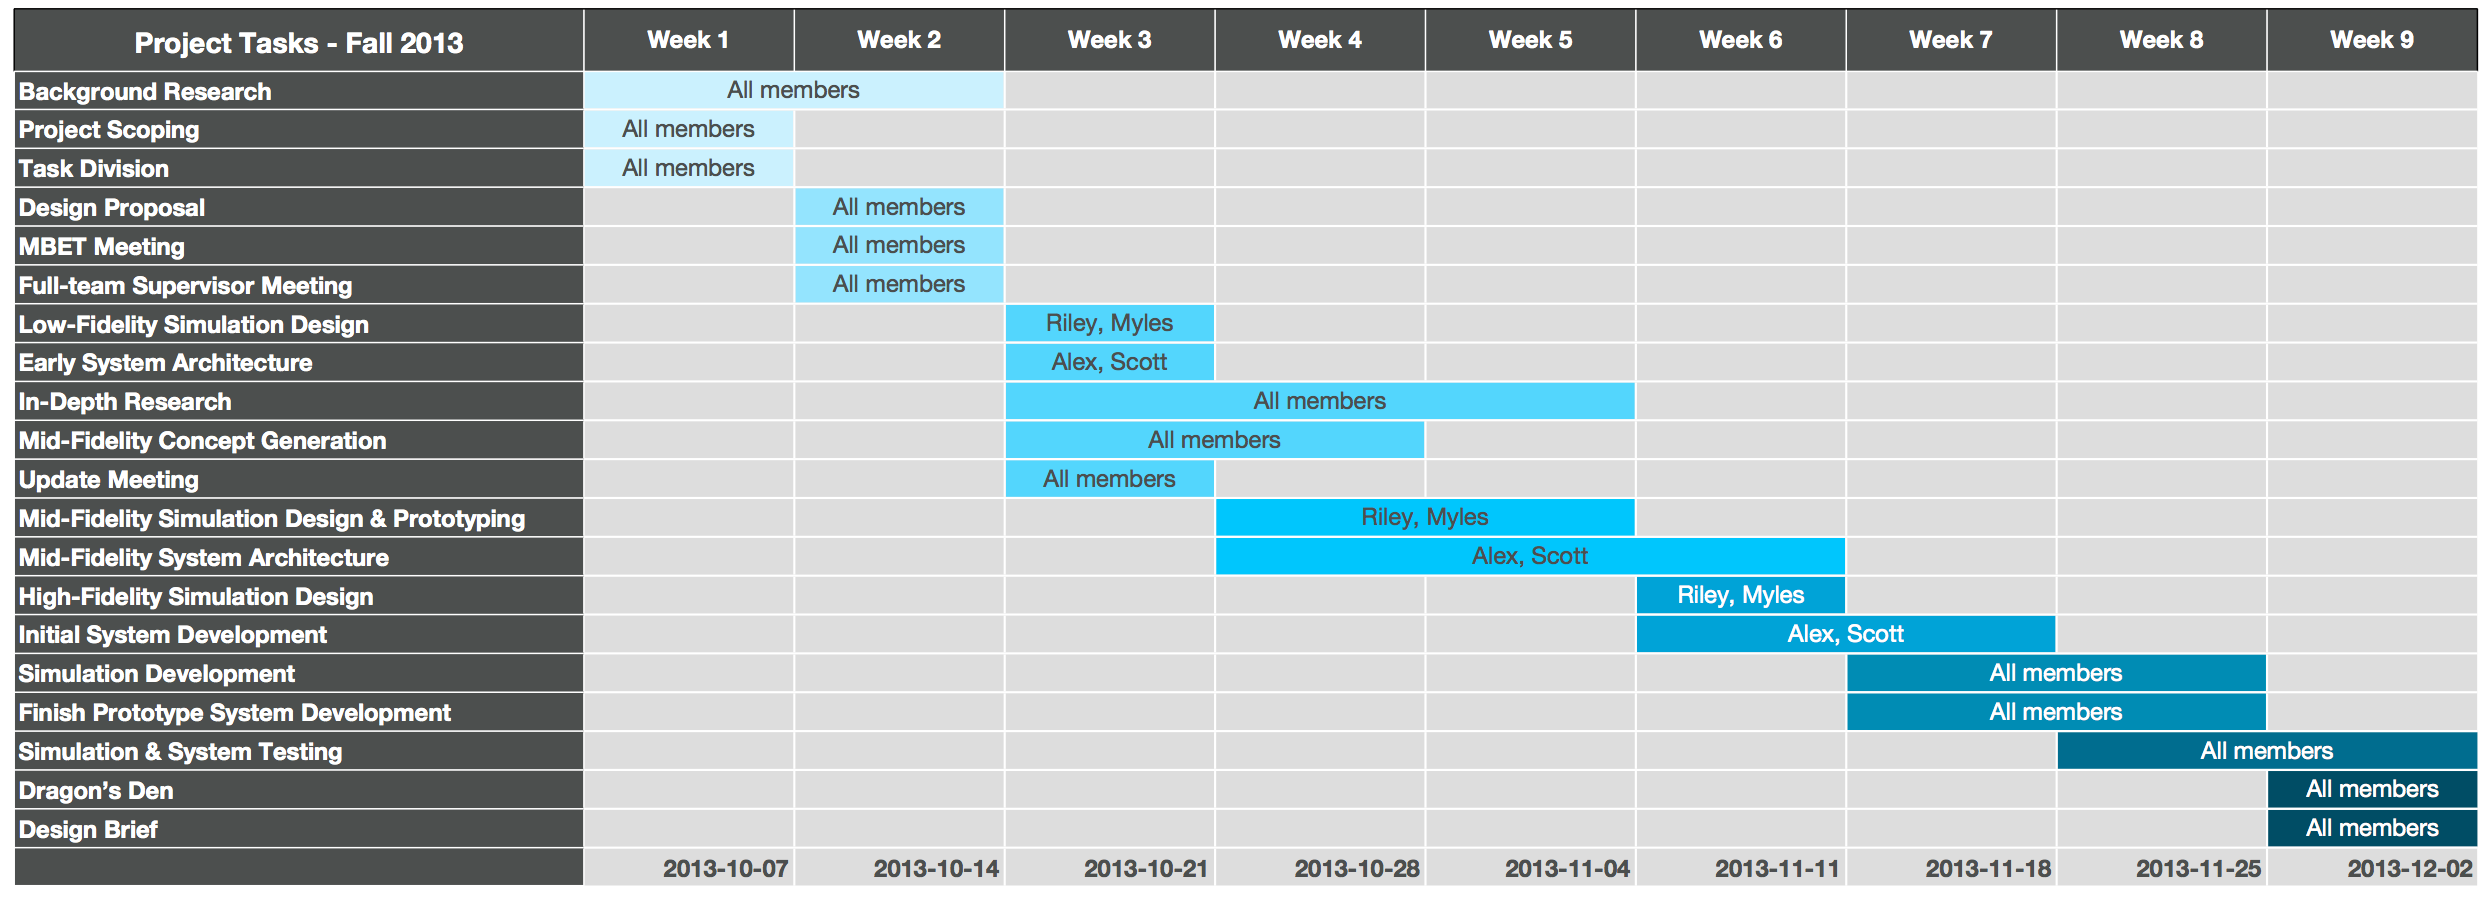
\includegraphics[scale=0.22, angle = 90]{figures/gantt-fall.png}
\caption{Gantt Chart for Fall 2013.}
\label{fig:gantt-fall}
\end{figure}

\newpage
\subsection{Gantt Chart}
\begin{figure}[H]
  \begin{centering}
    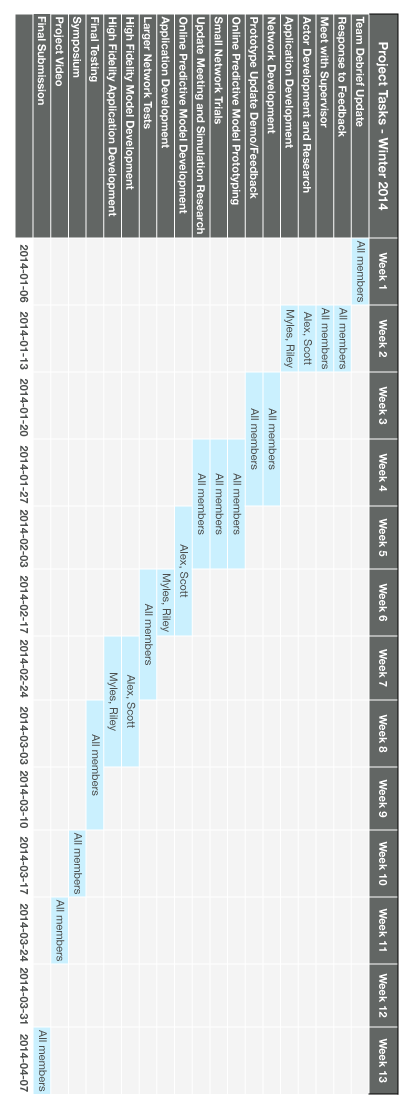
\includegraphics[scale=0.5, angle=180]{figures/gantt-vertical.png}
    \caption{Gantt Chart for Winter 2014}
    \label{fig:gantt-winter}
  \end{centering}
\end{figure}

\subsection{Performance Review}
The team was able to meet all deadlines with the usage of grace days throughout both terms. It was found that the initial Gantt Charts did not provide effective division of the work, and often left confusion with respect to responsibilities. The team was effectively able to delegate work at needed, however this could have been avoided with more intensive application of the Gantt Chart methodology.

It was found that deadlines were often delayed between major milestones, such as reports, presentations and demostrations. This often lead to the compression of work into short periods of time leading up to the project. This was expected given the nature of the time frame for the team members, however further steps should be taken to minimize the impact of this in the future.

Throughout both terms, the team struggled to meet on a regular basis. This had a negative impact on the team's adherance to deadlines, communication, and ability to effectively delegate work. In the future, consistent meetings should be enforced to ensure the team's adherance to the project plan.

In conclusion, the team was able to successfully meet all major milestones, however various steps could be taken to improve flow of the project. 

\newpage
\section{Conclusion}
The creation of the Relay Network  has helped further the understanding and capabilities of adaptive traffic control... [ALEX talk some real shit]

Furthermore, the Relay Application has helped redefine the value of Adaptive Traffic Control System Interfaces. For Traffic Engineers, the Relay Application enables the shift of responsibility and value from signal timing and tweaking to network monitoring and informed planning. The Relay Application exposes rich information which was previously either impossible or extremely expensive to collect, greatly reducing the costs associated with maintaining the efficiecny of the transportation network. This information allows traffic engineers to know exactly what's going on in the network at any moment. Traffic engineers are thus able to adapt quickly to drastic changes in the network. Through the use of geospatial data visualizations, the Relay Application is able to reveal high-level traffic patterns, providing invaluble insight into the workings of a city's transportation network. Access to this kind of information has the potential to change the way public infrastructure decisions are made. This project should serve as a guide for the development of Adaptive Traffic Control System Interfaces in the future.

The push for democratized traffic data is a major goal for this project, and the Relay Application serves as a first major attempt to present infrastructure-quality traffic information to the public. The Relay Application allows the public to examine and understand the workings of their public infrastructure, encouraging a more informed and engaged population. This brings benefits to both parties, as the public office now has an educated audience for making infrastructure developments, and an observant body to maintain public office accountability. Furthermore, the availability of traffic infrastructure information has the potential to revolutionize navigation-based solutions, such as Google Maps route planning and GPS devices. In the future, every car could be given a travel route which optimizes not only its travel time, but that of the entire transportation network.


\newpage
\section{Appendix A: Expert Interview Transcripts}
\subsection{Marc Tan - IBI Group}
\emph{Who uses these interfaces?} \\
�
There are�really three users to the interface.
One is the traffic engineers who need to input calibrated timings.
This is usually done in a central system that controls all the traffic signals.
Second, there is technical staff to who follow directions from traffic engineers in order to change timings depending on the situation.
Finally, for the in field controllers, there are technicians who can actually hard code timings or fall back plans. \\ \\
�
\emph{What is their job, their goals?} \\
�
Traffic�engineers generally ``draw'' up signal timings plans.
This is usually done using some deterministic and non-deterministic models depending on the work (this is usually my work).
As systems become adaptive, the goal of the traffic engineer is to more so calibrate and set up the existing conditions of the network rather than drawing up particular definitive second by second timings.
Obviously the goal is to improve the flow of traffic.
Technical staff usually work in control centres changing signal timing plans as needed usually under the direction/instruction of a traffic engineer.�\\ \\
�
\emph{What are they trying to understand and what information do they need to accomplish that?} \\ 
Traffic engineers: generally they are trying to understand traffic flows.
Information needed to understand this is normally traffic counts typically in 1 hour samples.
Now we don't just look at traffic, pedestrian and cyclist volumes also play a major role in determining timings.
Other things to consider is the capability of the existing system and the communication channels available (i.e. are the traffic signals connected to a central system, can we change them from a central system, are there other factors at play (special timings for transit, cyclists, pedestrians, etc.), is there an adaptive system.

Technical staff: just need directions from traffic engineers for at what point they can implement certain plans.
Basically if traffic looks X bad put in Y plan.
The jobs of these people get mostly eliminated if an adaptive traffic signal system is implemented. \\ 

\noindent \emph{What tasks do they perform using the interface, or based off of information from that interface?} \\
The interface usually gives information through video cameras from the field and some times road surface loop detectors that measure speed and or number of vehicles.
With this information technicians and engineers can perform changes to the timings.
An adaptive system would use this to adjust timings as needed.
For a non-adaptive system, this information is collected and inputted into models in order to determine timings. \\

Some things about my experiences:
I have generally done work on developing timings through modelling efforts. I did work one work term in a traffic control centre in Ottawa and the way I described it above with technicians changing timings based on situations observed on the cameras is the norm.
Toronto runs a SCOOT system on a number of their�arterials, which requires a large calibration effort after installation but once its going, it works pretty ok.
The big issue is that these SCOOT systems are quite expensive, with all the detection that is required to run the system.

\subsection{Peter Kelley - Paradigm Transportation}
A) System/Network \\
You'd want to know what the overall experienced delay is.
To get this you need to know signal timing plans, and volume of vehicles.
To minimize overall delay, they implement coordinated signals (for instance University Ave).
As you drive the speed limit, you should be able to hit green on the next set of lights.
However this offer works better for 1 direction over another eastbound vs westbound (depending on which direction peak traffic is going).
A big problem for this is emergency vehicles that can control the signal to get priority, having the signals get back on cycle can take a while and overall negatively impacts traffic flow.

\noindent B) Individual Intersections \\
Biggest problem is providing protected movements when no one is there.
Often I'm sure you've seen an advanced left when no one is turning, so everyone sits and waits.
This is because during peak hours, the signal timing plan assigns a minimum amount of green time, and then will extend it, if more vehicles are there.
As well, there are maximum time lengths that will change the signal to red from green, even if there is more traffic coming through.
The information we like to know about a single intersection is the turning movement counts, the delay of the approaches (north, south, east, west), the queue lengths of vehicles, and the volume/capacity ratio.
These all serve as a means to determine the Level of Service of an intersection.
I hope this helps.

\newpage
\addcontentsline{toc}{section}{References}

\bibliographystyle{IEEEtran}

\bibliography{bib}

\end{document}
